% Capitolul 2: Rupturi structurale și modele neliniare
% Analiza avansată a seriilor de timp și previziune -- Programul de master Statistică aplicată și data science, anul I, semestrul 2, Academia de Studii Economice din București
% GENERAT de latex/build_chapter2.py -- modificați generatorul, nu acest fișier.

\newcommand{\coursename}{Analiza avansată a seriilor de timp și previziune}
\def\atslang{ro}
% Preambul comun ATS -- Analiza avansată a seriilor de timp și previziune / Advanced Time Series Analysis and Forecasting
% (Beamer, 16:9). Același design ca MFM, SFM și TSA (copiat din TSA, 5 octombrie 2026). Înainte de % Preambul comun ATS -- Analiza avansată a seriilor de timp și previziune / Advanced Time Series Analysis and Forecasting
% (Beamer, 16:9). Același design ca MFM, SFM și TSA (copiat din TSA, 5 octombrie 2026). Înainte de % Preambul comun ATS -- Analiza avansată a seriilor de timp și previziune / Advanced Time Series Analysis and Forecasting
% (Beamer, 16:9). Același design ca MFM, SFM și TSA (copiat din TSA, 5 octombrie 2026). Înainte de \input{../../latex/preamble} se definește
%   \newcommand{\coursename}{Advanced Time Series Analysis and Forecasting}          (EN)
%   \newcommand{\coursename}{Analiza avansată a seriilor de timp și previziune}       (RO)  și  \def\atslang{ro}
% Fișierele .tex se află în EN/Courses, EN/Seminars, RO/Cursuri, RO/Seminarii (două niveluri sub rădăcină).
% Deck-urile sînt generate de latex/build_chapterN.py / build_seminarN.py (vezi latex/ats_build.py).

\documentclass[9pt, aspectratio=169, t]{beamer}
\providecommand{\coursename}{Advanced Time Series Analysis and Forecasting}

% Ensure content fits on slides
\setbeamersize{text margin left=8mm, text margin right=8mm}
% Smaller institute font (title page)
\setbeamerfont{institute}{size=\footnotesize}

%=============================================================================
% THEME AND STYLE CONFIGURATION
%=============================================================================
\usetheme{default}
% Using default theme for clean header/footer control

% Color Palette (matching Redispatch PDF)
\definecolor{MainBlue}{RGB}{26, 58, 110}
\definecolor{AccentBlue}{RGB}{26, 58, 110}
\definecolor{IDAred}{RGB}{205, 0, 0}
\definecolor{DarkGray}{RGB}{51, 51, 51}
\definecolor{MediumGray}{RGB}{128, 128, 128}
\definecolor{LightGray}{RGB}{248, 248, 248}
\definecolor{VeryLightGray}{RGB}{235, 235, 235}
\definecolor{KeynoteGray}{RGB}{218, 218, 218}
\definecolor{SectionGray}{RGB}{120, 120, 120}
\definecolor{FooterGray}{RGB}{100, 100, 100}
\definecolor{Crimson}{RGB}{220, 53, 69}
\definecolor{Forest}{RGB}{46, 125, 50}
\definecolor{Amber}{RGB}{181, 133, 63}
\definecolor{Orange}{RGB}{230, 126, 34}
\definecolor{Purple}{RGB}{142, 68, 173}

% Gradient background (exact Keynote 315° gradient: white to RGB 218,218,218)
\setbeamertemplate{background}{%
    \begin{tikzpicture}[remember picture, overlay]
        \shade[shading=axis, shading angle=315,
        top color=white, bottom color=KeynoteGray]
        (current page.south west) rectangle (current page.north east);
    \end{tikzpicture}%
}
% Fallback solid color for compatibility
\setbeamercolor{background canvas}{bg=}

\setbeamercolor{palette primary}{bg=MainBlue, fg=white}
\setbeamercolor{palette secondary}{bg=MainBlue!85, fg=white}
\setbeamercolor{palette tertiary}{bg=MainBlue!70, fg=white}
\setbeamercolor{structure}{fg=MainBlue}
\setbeamercolor{title}{fg=IDAred}
\setbeamercolor{frametitle}{fg=IDAred, bg=}
\setbeamercolor{block title}{bg=MainBlue, fg=white}
\setbeamercolor{block body}{bg=VeryLightGray, fg=DarkGray}
\setbeamercolor{block title alerted}{bg=Crimson, fg=white}
\setbeamercolor{block body alerted}{bg=Crimson!8, fg=DarkGray}
\setbeamercolor{block title example}{bg=Forest, fg=white}
\setbeamercolor{block body example}{bg=Forest!8, fg=DarkGray}
\setbeamercolor{item}{fg=MainBlue}

% Footer colors (override Madrid theme blue)
\setbeamercolor{author in head/foot}{fg=FooterGray, bg=}
\setbeamercolor{title in head/foot}{fg=FooterGray, bg=}
\setbeamercolor{date in head/foot}{fg=FooterGray, bg=}
\setbeamercolor{section in head/foot}{fg=FooterGray, bg=}
\setbeamercolor{subsection in head/foot}{fg=FooterGray, bg=}

% Bullet styles (apply everywhere including blocks)
\setbeamertemplate{itemize item}{\color{MainBlue}$\boxdot$}
\setbeamertemplate{itemize subitem}{\color{MainBlue}$\blacktriangleright$}
\setbeamertemplate{itemize subsubitem}{\color{MainBlue}\tiny$\bullet$}
\setbeamertemplate{itemize/enumerate body begin}{\normalsize}
\setbeamertemplate{itemize/enumerate subbody begin}{\normalsize}

% Item spacing - compact style
\setlength{\leftmargini}{10pt}       % Level 1: minimal indent
\setlength{\leftmarginii}{10pt}      % Level 2: minimal additional indent
% Compact list spacing (zero extra space before/after lists in blocks)
\makeatletter
\def\@listi{\leftmargin\leftmargini \topsep 0pt \parsep 0pt \itemsep 0pt}
\def\@listii{\leftmargin\leftmarginii \topsep 0pt \parsep 0pt \itemsep 0pt}
\makeatother

\setbeamertemplate{navigation symbols}{}

%=============================================================================
% CUSTOM HEADLINE
%=============================================================================
\setbeamertemplate{headline}{%
    \vskip10pt%
    \hbox to \paperwidth{%
        \hskip0.5cm%
        {\small\color{FooterGray}\renewcommand{\hyperlink}[2]{##2}\insertsectionhead}%
        \hfill%
        \textcolor{FooterGray}{\small\insertframenumber}%
        \hskip0.5cm%
    }%
    \vskip4pt%
    {\color{FooterGray}\hrule height 0.4pt}%
}

%=============================================================================
% CUSTOM FOOTER
%=============================================================================
\usepackage{fontawesome5}

\setbeamertemplate{footline}{%
    {\color{FooterGray}\hrule height 0.4pt}%
    \vskip4pt%
    \hbox to \paperwidth{%
        \hskip0.5cm%
        \textcolor{FooterGray}{\small\coursename}%
        \hfill%
        \raisebox{-0.1em}{%
            \begin{tikzpicture}[x=0.08em, y=0.08em, line width=0.4pt]
                \draw[FooterGray] (0,3) -- (1,4) -- (2,3.5) -- (3,5) -- (4,4) -- (5,6) -- (6,5.5) -- (7,4) -- (8,5) -- (9,7) -- (10,6) -- (11,5) -- (12,6.5) -- (13,8) -- (14,7) -- (15,6) -- (16,7.5) -- (17,9) -- (18,8) -- (19,7) -- (20,8.5) -- (21,10) -- (22,9) -- (23,8) -- (24,9.5);
            \end{tikzpicture}%
        }%
        \hskip0.5cm%
    }%
    \vskip6pt%
}

%=============================================================================
% PACKAGES
%=============================================================================
\usepackage[utf8]{inputenc}
\DeclareUnicodeCharacter{03B1}{\ensuremath{\alpha}}
\usepackage[T1]{fontenc}
\usepackage{amsmath, amssymb, amsthm}
\usepackage{mathtools}
\usepackage{bm}
\usepackage{tikz}
\usetikzlibrary{arrows.meta, positioning, shapes, calc, decorations.pathreplacing, shadings}
\usepackage{booktabs}
\usepackage{multirow}
\usepackage{array}
\usepackage{graphicx}
\usepackage{animate}
\usepackage{hyperref}
\usepackage{colortbl}
\usepackage{listings}
\lstset{language=Python, basicstyle=\ttfamily\scriptsize, keywordstyle=\color{MainBlue}\bfseries,
  commentstyle=\color{Forest}, stringstyle=\color{Crimson}, breaklines=true,
  frame=none, backgroundcolor=\color{VeryLightGray}, xleftmargin=2mm}
\hypersetup{colorlinks=true, linkcolor=MainBlue, urlcolor=MainBlue}
\graphicspath{{../../logos/}{../../charts/}{../../photos/}}
\usepackage{xcolor}
\hfuzz=2pt  % Suppress tiny overfull warnings (<2pt)
\vfuzz=2pt  % Suppress tiny vertical overfull warnings (<2pt)

%=============================================================================
% QUANTLET COMMANDS
%   \quantlet{<displayed name>}{<url>}       (generic)
%   \atsquantlet{Ch_05}{ATS_ch5_garch}       -> https://github.com/danpele/Advanced-Time-Series/tree/main/Quantlets/Ch_05/ATS_ch5_garch
%   \qlurl{<folder>} is defined per chapter by the generator (Quantlets/Ch_NN/<folder>)
%=============================================================================
\newcommand{\atsrepo}{https://github.com/danpele/Advanced-Time-Series}
\newcommand{\atsqlbase}{https://github.com/danpele/Advanced-Time-Series/tree/main/Quantlets}
\newcommand{\quantlet}[2]{%
    \hfill\href{#2}{%
        \raisebox{-0.15em}{
\includegraphics[height=0.7em]{ql_logo.png}}%
        \textcolor{MainBlue}{\tiny\ #1}%
    }%
}
\newcommand{\atsquantlet}[2]{\quantlet{\detokenize{#2}}{\atsqlbase/#1/#2}}

%=============================================================================
% NOTEBOOKS (Google Colab)
%   \colaburl{notebooks/EN/chapter5_seminar_notebook.ipynb} -> the Colab link of a file in the ATS repo
%   \nb: the chapter notebook (each seminar deck redefines it with \renewcommand)
%=============================================================================
\newcommand{\colaburl}[1]{https://colab.research.google.com/github/danpele/Advanced-Time-Series/blob/main/#1}
\newcommand{\nb}{https://colab.research.google.com/github/danpele/Advanced-Time-Series/tree/main/notebooks/EN}
\newcommand{\nbname}{notebooks/EN}

%=============================================================================
% SLIDE HELPERS (used by the generators; the same as in MFM)
%=============================================================================
% local font size for list bodies (the preamble forces \normalsize)
\newcommand{\itemsize}[1]{\setbeamertemplate{itemize/enumerate body begin}{#1}\setbeamertemplate{itemize/enumerate subbody begin}{#1}}
\newcommand{\intitle}[1]{{\hypersetup{urlcolor=white}#1}}   % white links inside coloured title bars
\newcommand{\imgcap}[1]{{\scriptsize #1}\\[0.5mm]}          % caption under a photo
\newcommand{\imgcredit}[2]{{\tiny\color{FooterGray}\href{#1}{#2}}}   % image credit: source URL, author/licence
\newcommand{\aiprompt}[1]{{\ttfamily\color{MainBlue}#1}}     % a prompt to an AI assistant

%=============================================================================
% SEMINARS: student version by default; the instructor wrapper *_solutions.tex sets \solutionstrue
%=============================================================================
\makeatletter\@ifundefined{ifsolutions}{\expandafter\newif\csname ifsolutions\endcsname}{}\makeatother
\newcommand{\solonly}[1]{\ifsolutions #1\fi}
\newcommand{\propsub}{\ifsolutions\else\framesubtitle{\ifdefined\atslang Rezolvarea se discută la seminar\else Solution discussed in class\fi}\fi}

%=============================================================================
% APPENDIX AND CHAPTER LINKS (latex/appendix_links.py writes the calls; it also re-declares these
% macros before \begin{document}, so the decks compile with or without this preamble block)
%=============================================================================
\providecommand{\atsapplink}[3]{\hypertarget{#2}{}\hyperlink{#1}{\beamergotobutton{#3}}}
\providecommand{\atsappback}[2]{\begin{tikzpicture}[remember picture,overlay]\node[anchor=south east] at ([xshift=-3mm,yshift=7mm]current page.south east){\hyperlink{#1}{\beamerreturnbutton{#2}}};\end{tikzpicture}}
\providecommand{\atschlink}[2]{\href{#1}{#2}}
\providecommand{\atschlinkt}[2]{\href{#1}{\usebeamercolor[fg]{frametitle}#2}}

%=============================================================================
% QUANTINAR COMMAND: link către un curs Quantinar (subiecte avansate)
%=============================================================================
\newcommand{\quantinar}[2]{%
    \href{#2}{%
        \raisebox{-0.15em}{
\includegraphics[height=0.8em]{qr_logo.png}}%
        \textcolor{MainBlue}{\scriptsize\ #1}%
    }%
}

%=============================================================================
% CUSTOM TITLE PAGE
%=============================================================================
\defbeamertemplate*{title page}{hybrid}[1][]
{
    \vspace{0.2cm}
    % Logos row - top header (with clickable links)
    \begin{center}
        \href{https://www.ase.ro}{
\includegraphics[height=1.0cm]{ase_logo.png}}\hspace{0.3cm}%
        \href{https://theida.net}{
\includegraphics[height=1.0cm]{ida_logo.png}}\hspace{0.3cm}%
        \href{https://blockchain-research-center.com}{
\includegraphics[height=1.0cm]{brc_logo.png}}\hspace{0.3cm}%
        \href{https://www.ai4efin.ase.ro}{
\includegraphics[height=1.0cm]{ai4efin_logo.png}}\hspace{0.3cm}%
        \href{https://ipe.ro/new}{
\includegraphics[height=1.0cm]{acad_logo.png}}\hspace{0.3cm}%
        \href{https://www.digital-finance-msca.com}{
\includegraphics[height=1.0cm]{msca_logo.png}}%
    \end{center}

    \vspace{0.6cm}

    % Main title with Q logos on sides (with clickable links)
    \begin{center}
        \begin{minipage}{0.1\textwidth}
            \centering
            \href{https://quantlet.com}{
\includegraphics[height=1.1cm]{ql_logo.png}}
        \end{minipage}%
        \begin{minipage}{0.78\textwidth}
            \centering
            {\LARGE\bfseries\usebeamercolor[fg]{title}\inserttitle}

            \vspace{0.3cm}

            {\usebeamerfont{subtitle}\usebeamercolor[fg]{title}\insertsubtitle}
        \end{minipage}%
        \begin{minipage}{0.1\textwidth}
            \centering
            \href{https://quantinar.com}{
\includegraphics[height=1.1cm]{qr_logo.png}}
        \end{minipage}
    \end{center}

    \vspace{0.6cm}

    % Authors (left aligned)
    \hspace{0.5cm}{\usebeamerfont{author}\insertauthor}

    \vspace{0.3cm}

    % Institute/Affiliations (left aligned)
    \hspace{0.5cm}\begin{minipage}[t]{0.9\textwidth}
        \raggedright\small\insertinstitute
    \end{minipage}
}

%=============================================================================
% THEOREM ENVIRONMENTS
%=============================================================================
\theoremstyle{definition}
\setbeamertemplate{theorems}[numbered]
\ifdefined\atslang
\newtheorem{defn}{Definiție}
\newtheorem{thm}{Teoremă}
\newtheorem{prop}{Propoziție}
\newtheorem{rmk}{Observație}
\else
\newtheorem{defn}{Definition}
\newtheorem{thm}{Theorem}
\newtheorem{prop}{Proposition}
\newtheorem{rmk}{Remark}
\fi

%=============================================================================
% CENTRED MINIPAGE (no extra vertical space)
%=============================================================================
\newenvironment{cminipage}[1]{%
    \par\noindent\hfill\begin{minipage}{#1}\ignorespaces
}{%
    \end{minipage}\hfill\null\par
}

%=============================================================================
% CUSTOM COMMANDS
%=============================================================================
\newcommand{\E}{\mathbb{E}}
\newcommand{\Var}{\text{Var}}
\newcommand{\Cov}{\text{Cov}}
\newcommand{\Corr}{\text{Corr}}
\newcommand{\R}{\mathbb{R}}
\newcommand{\N}{\mathbb{N}}
\newcommand{\Z}{\mathbb{Z}}
\newcommand{\B}{\mathbf{B}}
\newcommand{\imark}{\textcolor{MainBlue}{\textbullet}}
\newcommand{\RMSE}{\text{RMSE}}
\newcommand{\MAE}{\text{MAE}}
\newcommand{\MAPE}{\text{MAPE}}

% Boldface vector/matrix commands (VAR, VECM, state space)
\newcommand{\bY}{\mathbf{Y}}
\newcommand{\bX}{\mathbf{X}}
\newcommand{\bA}{\mathbf{A}}
\newcommand{\bB}{\mathbf{B}}
\newcommand{\bepsilon}{\boldsymbol{\varepsilon}}
\newcommand{\bSigma}{\boldsymbol{\Sigma}}
\newcommand{\bPhi}{\boldsymbol{\Phi}}
\newcommand{\bGamma}{\boldsymbol{\Gamma}}
\newcommand{\bPi}{\boldsymbol{\Pi}}
\newcommand{\bc}{\mathbf{c}}
\newcommand{\balpha}{\boldsymbol{\alpha}}
\newcommand{\bbeta}{\boldsymbol{\beta}}
\newcommand{\bvarepsilon}{\boldsymbol{\varepsilon}}

% Seminar marks
\newcommand{\correct}{\textcolor{Forest}{\checkmark}}
\newcommand{\incorrect}{\textcolor{Crimson}{\texttimes}}
 se definește
%   \newcommand{\coursename}{Advanced Time Series Analysis and Forecasting}          (EN)
%   \newcommand{\coursename}{Analiza avansată a seriilor de timp și previziune}       (RO)  și  \def\atslang{ro}
% Fișierele .tex se află în EN/Courses, EN/Seminars, RO/Cursuri, RO/Seminarii (două niveluri sub rădăcină).
% Deck-urile sînt generate de latex/build_chapterN.py / build_seminarN.py (vezi latex/ats_build.py).

\documentclass[9pt, aspectratio=169, t]{beamer}
\providecommand{\coursename}{Advanced Time Series Analysis and Forecasting}

% Ensure content fits on slides
\setbeamersize{text margin left=8mm, text margin right=8mm}
% Smaller institute font (title page)
\setbeamerfont{institute}{size=\footnotesize}

%=============================================================================
% THEME AND STYLE CONFIGURATION
%=============================================================================
\usetheme{default}
% Using default theme for clean header/footer control

% Color Palette (matching Redispatch PDF)
\definecolor{MainBlue}{RGB}{26, 58, 110}
\definecolor{AccentBlue}{RGB}{26, 58, 110}
\definecolor{IDAred}{RGB}{205, 0, 0}
\definecolor{DarkGray}{RGB}{51, 51, 51}
\definecolor{MediumGray}{RGB}{128, 128, 128}
\definecolor{LightGray}{RGB}{248, 248, 248}
\definecolor{VeryLightGray}{RGB}{235, 235, 235}
\definecolor{KeynoteGray}{RGB}{218, 218, 218}
\definecolor{SectionGray}{RGB}{120, 120, 120}
\definecolor{FooterGray}{RGB}{100, 100, 100}
\definecolor{Crimson}{RGB}{220, 53, 69}
\definecolor{Forest}{RGB}{46, 125, 50}
\definecolor{Amber}{RGB}{181, 133, 63}
\definecolor{Orange}{RGB}{230, 126, 34}
\definecolor{Purple}{RGB}{142, 68, 173}

% Gradient background (exact Keynote 315° gradient: white to RGB 218,218,218)
\setbeamertemplate{background}{%
    \begin{tikzpicture}[remember picture, overlay]
        \shade[shading=axis, shading angle=315,
        top color=white, bottom color=KeynoteGray]
        (current page.south west) rectangle (current page.north east);
    \end{tikzpicture}%
}
% Fallback solid color for compatibility
\setbeamercolor{background canvas}{bg=}

\setbeamercolor{palette primary}{bg=MainBlue, fg=white}
\setbeamercolor{palette secondary}{bg=MainBlue!85, fg=white}
\setbeamercolor{palette tertiary}{bg=MainBlue!70, fg=white}
\setbeamercolor{structure}{fg=MainBlue}
\setbeamercolor{title}{fg=IDAred}
\setbeamercolor{frametitle}{fg=IDAred, bg=}
\setbeamercolor{block title}{bg=MainBlue, fg=white}
\setbeamercolor{block body}{bg=VeryLightGray, fg=DarkGray}
\setbeamercolor{block title alerted}{bg=Crimson, fg=white}
\setbeamercolor{block body alerted}{bg=Crimson!8, fg=DarkGray}
\setbeamercolor{block title example}{bg=Forest, fg=white}
\setbeamercolor{block body example}{bg=Forest!8, fg=DarkGray}
\setbeamercolor{item}{fg=MainBlue}

% Footer colors (override Madrid theme blue)
\setbeamercolor{author in head/foot}{fg=FooterGray, bg=}
\setbeamercolor{title in head/foot}{fg=FooterGray, bg=}
\setbeamercolor{date in head/foot}{fg=FooterGray, bg=}
\setbeamercolor{section in head/foot}{fg=FooterGray, bg=}
\setbeamercolor{subsection in head/foot}{fg=FooterGray, bg=}

% Bullet styles (apply everywhere including blocks)
\setbeamertemplate{itemize item}{\color{MainBlue}$\boxdot$}
\setbeamertemplate{itemize subitem}{\color{MainBlue}$\blacktriangleright$}
\setbeamertemplate{itemize subsubitem}{\color{MainBlue}\tiny$\bullet$}
\setbeamertemplate{itemize/enumerate body begin}{\normalsize}
\setbeamertemplate{itemize/enumerate subbody begin}{\normalsize}

% Item spacing - compact style
\setlength{\leftmargini}{10pt}       % Level 1: minimal indent
\setlength{\leftmarginii}{10pt}      % Level 2: minimal additional indent
% Compact list spacing (zero extra space before/after lists in blocks)
\makeatletter
\def\@listi{\leftmargin\leftmargini \topsep 0pt \parsep 0pt \itemsep 0pt}
\def\@listii{\leftmargin\leftmarginii \topsep 0pt \parsep 0pt \itemsep 0pt}
\makeatother

\setbeamertemplate{navigation symbols}{}

%=============================================================================
% CUSTOM HEADLINE
%=============================================================================
\setbeamertemplate{headline}{%
    \vskip10pt%
    \hbox to \paperwidth{%
        \hskip0.5cm%
        {\small\color{FooterGray}\renewcommand{\hyperlink}[2]{##2}\insertsectionhead}%
        \hfill%
        \textcolor{FooterGray}{\small\insertframenumber}%
        \hskip0.5cm%
    }%
    \vskip4pt%
    {\color{FooterGray}\hrule height 0.4pt}%
}

%=============================================================================
% CUSTOM FOOTER
%=============================================================================
\usepackage{fontawesome5}

\setbeamertemplate{footline}{%
    {\color{FooterGray}\hrule height 0.4pt}%
    \vskip4pt%
    \hbox to \paperwidth{%
        \hskip0.5cm%
        \textcolor{FooterGray}{\small\coursename}%
        \hfill%
        \raisebox{-0.1em}{%
            \begin{tikzpicture}[x=0.08em, y=0.08em, line width=0.4pt]
                \draw[FooterGray] (0,3) -- (1,4) -- (2,3.5) -- (3,5) -- (4,4) -- (5,6) -- (6,5.5) -- (7,4) -- (8,5) -- (9,7) -- (10,6) -- (11,5) -- (12,6.5) -- (13,8) -- (14,7) -- (15,6) -- (16,7.5) -- (17,9) -- (18,8) -- (19,7) -- (20,8.5) -- (21,10) -- (22,9) -- (23,8) -- (24,9.5);
            \end{tikzpicture}%
        }%
        \hskip0.5cm%
    }%
    \vskip6pt%
}

%=============================================================================
% PACKAGES
%=============================================================================
\usepackage[utf8]{inputenc}
\DeclareUnicodeCharacter{03B1}{\ensuremath{\alpha}}
\usepackage[T1]{fontenc}
\usepackage{amsmath, amssymb, amsthm}
\usepackage{mathtools}
\usepackage{bm}
\usepackage{tikz}
\usetikzlibrary{arrows.meta, positioning, shapes, calc, decorations.pathreplacing, shadings}
\usepackage{booktabs}
\usepackage{multirow}
\usepackage{array}
\usepackage{graphicx}
\usepackage{animate}
\usepackage{hyperref}
\usepackage{colortbl}
\usepackage{listings}
\lstset{language=Python, basicstyle=\ttfamily\scriptsize, keywordstyle=\color{MainBlue}\bfseries,
  commentstyle=\color{Forest}, stringstyle=\color{Crimson}, breaklines=true,
  frame=none, backgroundcolor=\color{VeryLightGray}, xleftmargin=2mm}
\hypersetup{colorlinks=true, linkcolor=MainBlue, urlcolor=MainBlue}
\graphicspath{{../../logos/}{../../charts/}{../../photos/}}
\usepackage{xcolor}
\hfuzz=2pt  % Suppress tiny overfull warnings (<2pt)
\vfuzz=2pt  % Suppress tiny vertical overfull warnings (<2pt)

%=============================================================================
% QUANTLET COMMANDS
%   \quantlet{<displayed name>}{<url>}       (generic)
%   \atsquantlet{Ch_05}{ATS_ch5_garch}       -> https://github.com/danpele/Advanced-Time-Series/tree/main/Quantlets/Ch_05/ATS_ch5_garch
%   \qlurl{<folder>} is defined per chapter by the generator (Quantlets/Ch_NN/<folder>)
%=============================================================================
\newcommand{\atsrepo}{https://github.com/danpele/Advanced-Time-Series}
\newcommand{\atsqlbase}{https://github.com/danpele/Advanced-Time-Series/tree/main/Quantlets}
\newcommand{\quantlet}[2]{%
    \hfill\href{#2}{%
        \raisebox{-0.15em}{
\includegraphics[height=0.7em]{ql_logo.png}}%
        \textcolor{MainBlue}{\tiny\ #1}%
    }%
}
\newcommand{\atsquantlet}[2]{\quantlet{\detokenize{#2}}{\atsqlbase/#1/#2}}

%=============================================================================
% NOTEBOOKS (Google Colab)
%   \colaburl{notebooks/EN/chapter5_seminar_notebook.ipynb} -> the Colab link of a file in the ATS repo
%   \nb: the chapter notebook (each seminar deck redefines it with \renewcommand)
%=============================================================================
\newcommand{\colaburl}[1]{https://colab.research.google.com/github/danpele/Advanced-Time-Series/blob/main/#1}
\newcommand{\nb}{https://colab.research.google.com/github/danpele/Advanced-Time-Series/tree/main/notebooks/EN}
\newcommand{\nbname}{notebooks/EN}

%=============================================================================
% SLIDE HELPERS (used by the generators; the same as in MFM)
%=============================================================================
% local font size for list bodies (the preamble forces \normalsize)
\newcommand{\itemsize}[1]{\setbeamertemplate{itemize/enumerate body begin}{#1}\setbeamertemplate{itemize/enumerate subbody begin}{#1}}
\newcommand{\intitle}[1]{{\hypersetup{urlcolor=white}#1}}   % white links inside coloured title bars
\newcommand{\imgcap}[1]{{\scriptsize #1}\\[0.5mm]}          % caption under a photo
\newcommand{\imgcredit}[2]{{\tiny\color{FooterGray}\href{#1}{#2}}}   % image credit: source URL, author/licence
\newcommand{\aiprompt}[1]{{\ttfamily\color{MainBlue}#1}}     % a prompt to an AI assistant

%=============================================================================
% SEMINARS: student version by default; the instructor wrapper *_solutions.tex sets \solutionstrue
%=============================================================================
\makeatletter\@ifundefined{ifsolutions}{\expandafter\newif\csname ifsolutions\endcsname}{}\makeatother
\newcommand{\solonly}[1]{\ifsolutions #1\fi}
\newcommand{\propsub}{\ifsolutions\else\framesubtitle{\ifdefined\atslang Rezolvarea se discută la seminar\else Solution discussed in class\fi}\fi}

%=============================================================================
% APPENDIX AND CHAPTER LINKS (latex/appendix_links.py writes the calls; it also re-declares these
% macros before \begin{document}, so the decks compile with or without this preamble block)
%=============================================================================
\providecommand{\atsapplink}[3]{\hypertarget{#2}{}\hyperlink{#1}{\beamergotobutton{#3}}}
\providecommand{\atsappback}[2]{\begin{tikzpicture}[remember picture,overlay]\node[anchor=south east] at ([xshift=-3mm,yshift=7mm]current page.south east){\hyperlink{#1}{\beamerreturnbutton{#2}}};\end{tikzpicture}}
\providecommand{\atschlink}[2]{\href{#1}{#2}}
\providecommand{\atschlinkt}[2]{\href{#1}{\usebeamercolor[fg]{frametitle}#2}}

%=============================================================================
% QUANTINAR COMMAND: link către un curs Quantinar (subiecte avansate)
%=============================================================================
\newcommand{\quantinar}[2]{%
    \href{#2}{%
        \raisebox{-0.15em}{
\includegraphics[height=0.8em]{qr_logo.png}}%
        \textcolor{MainBlue}{\scriptsize\ #1}%
    }%
}

%=============================================================================
% CUSTOM TITLE PAGE
%=============================================================================
\defbeamertemplate*{title page}{hybrid}[1][]
{
    \vspace{0.2cm}
    % Logos row - top header (with clickable links)
    \begin{center}
        \href{https://www.ase.ro}{
\includegraphics[height=1.0cm]{ase_logo.png}}\hspace{0.3cm}%
        \href{https://theida.net}{
\includegraphics[height=1.0cm]{ida_logo.png}}\hspace{0.3cm}%
        \href{https://blockchain-research-center.com}{
\includegraphics[height=1.0cm]{brc_logo.png}}\hspace{0.3cm}%
        \href{https://www.ai4efin.ase.ro}{
\includegraphics[height=1.0cm]{ai4efin_logo.png}}\hspace{0.3cm}%
        \href{https://ipe.ro/new}{
\includegraphics[height=1.0cm]{acad_logo.png}}\hspace{0.3cm}%
        \href{https://www.digital-finance-msca.com}{
\includegraphics[height=1.0cm]{msca_logo.png}}%
    \end{center}

    \vspace{0.6cm}

    % Main title with Q logos on sides (with clickable links)
    \begin{center}
        \begin{minipage}{0.1\textwidth}
            \centering
            \href{https://quantlet.com}{
\includegraphics[height=1.1cm]{ql_logo.png}}
        \end{minipage}%
        \begin{minipage}{0.78\textwidth}
            \centering
            {\LARGE\bfseries\usebeamercolor[fg]{title}\inserttitle}

            \vspace{0.3cm}

            {\usebeamerfont{subtitle}\usebeamercolor[fg]{title}\insertsubtitle}
        \end{minipage}%
        \begin{minipage}{0.1\textwidth}
            \centering
            \href{https://quantinar.com}{
\includegraphics[height=1.1cm]{qr_logo.png}}
        \end{minipage}
    \end{center}

    \vspace{0.6cm}

    % Authors (left aligned)
    \hspace{0.5cm}{\usebeamerfont{author}\insertauthor}

    \vspace{0.3cm}

    % Institute/Affiliations (left aligned)
    \hspace{0.5cm}\begin{minipage}[t]{0.9\textwidth}
        \raggedright\small\insertinstitute
    \end{minipage}
}

%=============================================================================
% THEOREM ENVIRONMENTS
%=============================================================================
\theoremstyle{definition}
\setbeamertemplate{theorems}[numbered]
\ifdefined\atslang
\newtheorem{defn}{Definiție}
\newtheorem{thm}{Teoremă}
\newtheorem{prop}{Propoziție}
\newtheorem{rmk}{Observație}
\else
\newtheorem{defn}{Definition}
\newtheorem{thm}{Theorem}
\newtheorem{prop}{Proposition}
\newtheorem{rmk}{Remark}
\fi

%=============================================================================
% CENTRED MINIPAGE (no extra vertical space)
%=============================================================================
\newenvironment{cminipage}[1]{%
    \par\noindent\hfill\begin{minipage}{#1}\ignorespaces
}{%
    \end{minipage}\hfill\null\par
}

%=============================================================================
% CUSTOM COMMANDS
%=============================================================================
\newcommand{\E}{\mathbb{E}}
\newcommand{\Var}{\text{Var}}
\newcommand{\Cov}{\text{Cov}}
\newcommand{\Corr}{\text{Corr}}
\newcommand{\R}{\mathbb{R}}
\newcommand{\N}{\mathbb{N}}
\newcommand{\Z}{\mathbb{Z}}
\newcommand{\B}{\mathbf{B}}
\newcommand{\imark}{\textcolor{MainBlue}{\textbullet}}
\newcommand{\RMSE}{\text{RMSE}}
\newcommand{\MAE}{\text{MAE}}
\newcommand{\MAPE}{\text{MAPE}}

% Boldface vector/matrix commands (VAR, VECM, state space)
\newcommand{\bY}{\mathbf{Y}}
\newcommand{\bX}{\mathbf{X}}
\newcommand{\bA}{\mathbf{A}}
\newcommand{\bB}{\mathbf{B}}
\newcommand{\bepsilon}{\boldsymbol{\varepsilon}}
\newcommand{\bSigma}{\boldsymbol{\Sigma}}
\newcommand{\bPhi}{\boldsymbol{\Phi}}
\newcommand{\bGamma}{\boldsymbol{\Gamma}}
\newcommand{\bPi}{\boldsymbol{\Pi}}
\newcommand{\bc}{\mathbf{c}}
\newcommand{\balpha}{\boldsymbol{\alpha}}
\newcommand{\bbeta}{\boldsymbol{\beta}}
\newcommand{\bvarepsilon}{\boldsymbol{\varepsilon}}

% Seminar marks
\newcommand{\correct}{\textcolor{Forest}{\checkmark}}
\newcommand{\incorrect}{\textcolor{Crimson}{\texttimes}}
 se definește
%   \newcommand{\coursename}{Advanced Time Series Analysis and Forecasting}          (EN)
%   \newcommand{\coursename}{Analiza avansată a seriilor de timp și previziune}       (RO)  și  \def\atslang{ro}
% Fișierele .tex se află în EN/Courses, EN/Seminars, RO/Cursuri, RO/Seminarii (două niveluri sub rădăcină).
% Deck-urile sînt generate de latex/build_chapterN.py / build_seminarN.py (vezi latex/ats_build.py).

\documentclass[9pt, aspectratio=169, t]{beamer}
\providecommand{\coursename}{Advanced Time Series Analysis and Forecasting}

% Ensure content fits on slides
\setbeamersize{text margin left=8mm, text margin right=8mm}
% Smaller institute font (title page)
\setbeamerfont{institute}{size=\footnotesize}

%=============================================================================
% THEME AND STYLE CONFIGURATION
%=============================================================================
\usetheme{default}
% Using default theme for clean header/footer control

% Color Palette (matching Redispatch PDF)
\definecolor{MainBlue}{RGB}{26, 58, 110}
\definecolor{AccentBlue}{RGB}{26, 58, 110}
\definecolor{IDAred}{RGB}{205, 0, 0}
\definecolor{DarkGray}{RGB}{51, 51, 51}
\definecolor{MediumGray}{RGB}{128, 128, 128}
\definecolor{LightGray}{RGB}{248, 248, 248}
\definecolor{VeryLightGray}{RGB}{235, 235, 235}
\definecolor{KeynoteGray}{RGB}{218, 218, 218}
\definecolor{SectionGray}{RGB}{120, 120, 120}
\definecolor{FooterGray}{RGB}{100, 100, 100}
\definecolor{Crimson}{RGB}{220, 53, 69}
\definecolor{Forest}{RGB}{46, 125, 50}
\definecolor{Amber}{RGB}{181, 133, 63}
\definecolor{Orange}{RGB}{230, 126, 34}
\definecolor{Purple}{RGB}{142, 68, 173}

% Gradient background (exact Keynote 315° gradient: white to RGB 218,218,218)
\setbeamertemplate{background}{%
    \begin{tikzpicture}[remember picture, overlay]
        \shade[shading=axis, shading angle=315,
        top color=white, bottom color=KeynoteGray]
        (current page.south west) rectangle (current page.north east);
    \end{tikzpicture}%
}
% Fallback solid color for compatibility
\setbeamercolor{background canvas}{bg=}

\setbeamercolor{palette primary}{bg=MainBlue, fg=white}
\setbeamercolor{palette secondary}{bg=MainBlue!85, fg=white}
\setbeamercolor{palette tertiary}{bg=MainBlue!70, fg=white}
\setbeamercolor{structure}{fg=MainBlue}
\setbeamercolor{title}{fg=IDAred}
\setbeamercolor{frametitle}{fg=IDAred, bg=}
\setbeamercolor{block title}{bg=MainBlue, fg=white}
\setbeamercolor{block body}{bg=VeryLightGray, fg=DarkGray}
\setbeamercolor{block title alerted}{bg=Crimson, fg=white}
\setbeamercolor{block body alerted}{bg=Crimson!8, fg=DarkGray}
\setbeamercolor{block title example}{bg=Forest, fg=white}
\setbeamercolor{block body example}{bg=Forest!8, fg=DarkGray}
\setbeamercolor{item}{fg=MainBlue}

% Footer colors (override Madrid theme blue)
\setbeamercolor{author in head/foot}{fg=FooterGray, bg=}
\setbeamercolor{title in head/foot}{fg=FooterGray, bg=}
\setbeamercolor{date in head/foot}{fg=FooterGray, bg=}
\setbeamercolor{section in head/foot}{fg=FooterGray, bg=}
\setbeamercolor{subsection in head/foot}{fg=FooterGray, bg=}

% Bullet styles (apply everywhere including blocks)
\setbeamertemplate{itemize item}{\color{MainBlue}$\boxdot$}
\setbeamertemplate{itemize subitem}{\color{MainBlue}$\blacktriangleright$}
\setbeamertemplate{itemize subsubitem}{\color{MainBlue}\tiny$\bullet$}
\setbeamertemplate{itemize/enumerate body begin}{\normalsize}
\setbeamertemplate{itemize/enumerate subbody begin}{\normalsize}

% Item spacing - compact style
\setlength{\leftmargini}{10pt}       % Level 1: minimal indent
\setlength{\leftmarginii}{10pt}      % Level 2: minimal additional indent
% Compact list spacing (zero extra space before/after lists in blocks)
\makeatletter
\def\@listi{\leftmargin\leftmargini \topsep 0pt \parsep 0pt \itemsep 0pt}
\def\@listii{\leftmargin\leftmarginii \topsep 0pt \parsep 0pt \itemsep 0pt}
\makeatother

\setbeamertemplate{navigation symbols}{}

%=============================================================================
% CUSTOM HEADLINE
%=============================================================================
\setbeamertemplate{headline}{%
    \vskip10pt%
    \hbox to \paperwidth{%
        \hskip0.5cm%
        {\small\color{FooterGray}\renewcommand{\hyperlink}[2]{##2}\insertsectionhead}%
        \hfill%
        \textcolor{FooterGray}{\small\insertframenumber}%
        \hskip0.5cm%
    }%
    \vskip4pt%
    {\color{FooterGray}\hrule height 0.4pt}%
}

%=============================================================================
% CUSTOM FOOTER
%=============================================================================
\usepackage{fontawesome5}

\setbeamertemplate{footline}{%
    {\color{FooterGray}\hrule height 0.4pt}%
    \vskip4pt%
    \hbox to \paperwidth{%
        \hskip0.5cm%
        \textcolor{FooterGray}{\small\coursename}%
        \hfill%
        \raisebox{-0.1em}{%
            \begin{tikzpicture}[x=0.08em, y=0.08em, line width=0.4pt]
                \draw[FooterGray] (0,3) -- (1,4) -- (2,3.5) -- (3,5) -- (4,4) -- (5,6) -- (6,5.5) -- (7,4) -- (8,5) -- (9,7) -- (10,6) -- (11,5) -- (12,6.5) -- (13,8) -- (14,7) -- (15,6) -- (16,7.5) -- (17,9) -- (18,8) -- (19,7) -- (20,8.5) -- (21,10) -- (22,9) -- (23,8) -- (24,9.5);
            \end{tikzpicture}%
        }%
        \hskip0.5cm%
    }%
    \vskip6pt%
}

%=============================================================================
% PACKAGES
%=============================================================================
\usepackage[utf8]{inputenc}
\DeclareUnicodeCharacter{03B1}{\ensuremath{\alpha}}
\usepackage[T1]{fontenc}
\usepackage{amsmath, amssymb, amsthm}
\usepackage{mathtools}
\usepackage{bm}
\usepackage{tikz}
\usetikzlibrary{arrows.meta, positioning, shapes, calc, decorations.pathreplacing, shadings}
\usepackage{booktabs}
\usepackage{multirow}
\usepackage{array}
\usepackage{graphicx}
\usepackage{animate}
\usepackage{hyperref}
\usepackage{colortbl}
\usepackage{listings}
\lstset{language=Python, basicstyle=\ttfamily\scriptsize, keywordstyle=\color{MainBlue}\bfseries,
  commentstyle=\color{Forest}, stringstyle=\color{Crimson}, breaklines=true,
  frame=none, backgroundcolor=\color{VeryLightGray}, xleftmargin=2mm}
\hypersetup{colorlinks=true, linkcolor=MainBlue, urlcolor=MainBlue}
\graphicspath{{../../logos/}{../../charts/}{../../photos/}}
\usepackage{xcolor}
\hfuzz=2pt  % Suppress tiny overfull warnings (<2pt)
\vfuzz=2pt  % Suppress tiny vertical overfull warnings (<2pt)

%=============================================================================
% QUANTLET COMMANDS
%   \quantlet{<displayed name>}{<url>}       (generic)
%   \atsquantlet{Ch_05}{ATS_ch5_garch}       -> https://github.com/danpele/Advanced-Time-Series/tree/main/Quantlets/Ch_05/ATS_ch5_garch
%   \qlurl{<folder>} is defined per chapter by the generator (Quantlets/Ch_NN/<folder>)
%=============================================================================
\newcommand{\atsrepo}{https://github.com/danpele/Advanced-Time-Series}
\newcommand{\atsqlbase}{https://github.com/danpele/Advanced-Time-Series/tree/main/Quantlets}
\newcommand{\quantlet}[2]{%
    \hfill\href{#2}{%
        \raisebox{-0.15em}{
\includegraphics[height=0.7em]{ql_logo.png}}%
        \textcolor{MainBlue}{\tiny\ #1}%
    }%
}
\newcommand{\atsquantlet}[2]{\quantlet{\detokenize{#2}}{\atsqlbase/#1/#2}}

%=============================================================================
% NOTEBOOKS (Google Colab)
%   \colaburl{notebooks/EN/chapter5_seminar_notebook.ipynb} -> the Colab link of a file in the ATS repo
%   \nb: the chapter notebook (each seminar deck redefines it with \renewcommand)
%=============================================================================
\newcommand{\colaburl}[1]{https://colab.research.google.com/github/danpele/Advanced-Time-Series/blob/main/#1}
\newcommand{\nb}{https://colab.research.google.com/github/danpele/Advanced-Time-Series/tree/main/notebooks/EN}
\newcommand{\nbname}{notebooks/EN}

%=============================================================================
% SLIDE HELPERS (used by the generators; the same as in MFM)
%=============================================================================
% local font size for list bodies (the preamble forces \normalsize)
\newcommand{\itemsize}[1]{\setbeamertemplate{itemize/enumerate body begin}{#1}\setbeamertemplate{itemize/enumerate subbody begin}{#1}}
\newcommand{\intitle}[1]{{\hypersetup{urlcolor=white}#1}}   % white links inside coloured title bars
\newcommand{\imgcap}[1]{{\scriptsize #1}\\[0.5mm]}          % caption under a photo
\newcommand{\imgcredit}[2]{{\tiny\color{FooterGray}\href{#1}{#2}}}   % image credit: source URL, author/licence
\newcommand{\aiprompt}[1]{{\ttfamily\color{MainBlue}#1}}     % a prompt to an AI assistant

%=============================================================================
% SEMINARS: student version by default; the instructor wrapper *_solutions.tex sets \solutionstrue
%=============================================================================
\makeatletter\@ifundefined{ifsolutions}{\expandafter\newif\csname ifsolutions\endcsname}{}\makeatother
\newcommand{\solonly}[1]{\ifsolutions #1\fi}
\newcommand{\propsub}{\ifsolutions\else\framesubtitle{\ifdefined\atslang Rezolvarea se discută la seminar\else Solution discussed in class\fi}\fi}

%=============================================================================
% APPENDIX AND CHAPTER LINKS (latex/appendix_links.py writes the calls; it also re-declares these
% macros before \begin{document}, so the decks compile with or without this preamble block)
%=============================================================================
\providecommand{\atsapplink}[3]{\hypertarget{#2}{}\hyperlink{#1}{\beamergotobutton{#3}}}
\providecommand{\atsappback}[2]{\begin{tikzpicture}[remember picture,overlay]\node[anchor=south east] at ([xshift=-3mm,yshift=7mm]current page.south east){\hyperlink{#1}{\beamerreturnbutton{#2}}};\end{tikzpicture}}
\providecommand{\atschlink}[2]{\href{#1}{#2}}
\providecommand{\atschlinkt}[2]{\href{#1}{\usebeamercolor[fg]{frametitle}#2}}

%=============================================================================
% QUANTINAR COMMAND: link către un curs Quantinar (subiecte avansate)
%=============================================================================
\newcommand{\quantinar}[2]{%
    \href{#2}{%
        \raisebox{-0.15em}{
\includegraphics[height=0.8em]{qr_logo.png}}%
        \textcolor{MainBlue}{\scriptsize\ #1}%
    }%
}

%=============================================================================
% CUSTOM TITLE PAGE
%=============================================================================
\defbeamertemplate*{title page}{hybrid}[1][]
{
    \vspace{0.2cm}
    % Logos row - top header (with clickable links)
    \begin{center}
        \href{https://www.ase.ro}{
\includegraphics[height=1.0cm]{ase_logo.png}}\hspace{0.3cm}%
        \href{https://theida.net}{
\includegraphics[height=1.0cm]{ida_logo.png}}\hspace{0.3cm}%
        \href{https://blockchain-research-center.com}{
\includegraphics[height=1.0cm]{brc_logo.png}}\hspace{0.3cm}%
        \href{https://www.ai4efin.ase.ro}{
\includegraphics[height=1.0cm]{ai4efin_logo.png}}\hspace{0.3cm}%
        \href{https://ipe.ro/new}{
\includegraphics[height=1.0cm]{acad_logo.png}}\hspace{0.3cm}%
        \href{https://www.digital-finance-msca.com}{
\includegraphics[height=1.0cm]{msca_logo.png}}%
    \end{center}

    \vspace{0.6cm}

    % Main title with Q logos on sides (with clickable links)
    \begin{center}
        \begin{minipage}{0.1\textwidth}
            \centering
            \href{https://quantlet.com}{
\includegraphics[height=1.1cm]{ql_logo.png}}
        \end{minipage}%
        \begin{minipage}{0.78\textwidth}
            \centering
            {\LARGE\bfseries\usebeamercolor[fg]{title}\inserttitle}

            \vspace{0.3cm}

            {\usebeamerfont{subtitle}\usebeamercolor[fg]{title}\insertsubtitle}
        \end{minipage}%
        \begin{minipage}{0.1\textwidth}
            \centering
            \href{https://quantinar.com}{
\includegraphics[height=1.1cm]{qr_logo.png}}
        \end{minipage}
    \end{center}

    \vspace{0.6cm}

    % Authors (left aligned)
    \hspace{0.5cm}{\usebeamerfont{author}\insertauthor}

    \vspace{0.3cm}

    % Institute/Affiliations (left aligned)
    \hspace{0.5cm}\begin{minipage}[t]{0.9\textwidth}
        \raggedright\small\insertinstitute
    \end{minipage}
}

%=============================================================================
% THEOREM ENVIRONMENTS
%=============================================================================
\theoremstyle{definition}
\setbeamertemplate{theorems}[numbered]
\ifdefined\atslang
\newtheorem{defn}{Definiție}
\newtheorem{thm}{Teoremă}
\newtheorem{prop}{Propoziție}
\newtheorem{rmk}{Observație}
\else
\newtheorem{defn}{Definition}
\newtheorem{thm}{Theorem}
\newtheorem{prop}{Proposition}
\newtheorem{rmk}{Remark}
\fi

%=============================================================================
% CENTRED MINIPAGE (no extra vertical space)
%=============================================================================
\newenvironment{cminipage}[1]{%
    \par\noindent\hfill\begin{minipage}{#1}\ignorespaces
}{%
    \end{minipage}\hfill\null\par
}

%=============================================================================
% CUSTOM COMMANDS
%=============================================================================
\newcommand{\E}{\mathbb{E}}
\newcommand{\Var}{\text{Var}}
\newcommand{\Cov}{\text{Cov}}
\newcommand{\Corr}{\text{Corr}}
\newcommand{\R}{\mathbb{R}}
\newcommand{\N}{\mathbb{N}}
\newcommand{\Z}{\mathbb{Z}}
\newcommand{\B}{\mathbf{B}}
\newcommand{\imark}{\textcolor{MainBlue}{\textbullet}}
\newcommand{\RMSE}{\text{RMSE}}
\newcommand{\MAE}{\text{MAE}}
\newcommand{\MAPE}{\text{MAPE}}

% Boldface vector/matrix commands (VAR, VECM, state space)
\newcommand{\bY}{\mathbf{Y}}
\newcommand{\bX}{\mathbf{X}}
\newcommand{\bA}{\mathbf{A}}
\newcommand{\bB}{\mathbf{B}}
\newcommand{\bepsilon}{\boldsymbol{\varepsilon}}
\newcommand{\bSigma}{\boldsymbol{\Sigma}}
\newcommand{\bPhi}{\boldsymbol{\Phi}}
\newcommand{\bGamma}{\boldsymbol{\Gamma}}
\newcommand{\bPi}{\boldsymbol{\Pi}}
\newcommand{\bc}{\mathbf{c}}
\newcommand{\balpha}{\boldsymbol{\alpha}}
\newcommand{\bbeta}{\boldsymbol{\beta}}
\newcommand{\bvarepsilon}{\boldsymbol{\varepsilon}}

% Seminar marks
\newcommand{\correct}{\textcolor{Forest}{\checkmark}}
\newcommand{\incorrect}{\textcolor{Crimson}{\texttimes}}


\newcommand{\qlurl}[1]{https://github.com/danpele/Advanced-Time-Series/tree/main/Quantlets/Ch_02/#1}

% Clickable citations (DOIs verified via Crossref)
\newcommand{\refAnd}{\href{https://doi.org/10.2307/2951764}{Andrews (1993)}}
\newcommand{\refAP}{\href{https://doi.org/10.2307/2951753}{Andrews și Ploberger (1994)}}
\newcommand{\refBai}{\href{https://doi.org/10.1162/003465397557132}{Bai (1997)}}
\newcommand{\refBPa}{\href{https://doi.org/10.2307/2998540}{Bai și Perron (1998)}}
\newcommand{\refBPb}{\href{https://doi.org/10.1002/jae.659}{Bai și Perron (2003)}}
\newcommand{\refBF}{\href{https://doi.org/10.2307/2527284}{Balke și Fomby (1997)}}
\newcommand{\refBDSL}{\href{https://doi.org/10.1080/07474939608800353}{Brock et al.\ (1996)}}
\newcommand{\refBDE}{\href{https://doi.org/10.1111/j.2517-6161.1975.tb01532.x}{Brown, Durbin și Evans (1975)}}
\newcommand{\refCar}{\href{https://doi.org/10.1016/S0304-4076(02)00112-4}{Carrasco (2002)}}
\newcommand{\refCP}{\href{https://doi.org/10.1093/acrefore/9780190625979.013.179}{Casini și Perron (2019)}}
\newcommand{\refChan}{\href{https://doi.org/10.1214/aos/1176349040}{Chan (1993)}}
\newcommand{\refChow}{\href{https://doi.org/10.2307/1910133}{Chow (1960)}}
\newcommand{\refCHK}{\href{https://doi.org/10.1093/biomet/82.3.603}{Chu, Hornik și Kuan (1995)}}
\newcommand{\refCSW}{\href{https://doi.org/10.2307/2171955}{Chu, Stinchcombe și White (1996)}}
\newcommand{\refCFS}{\href{https://doi.org/10.1016/j.ijforecast.2003.10.004}{Clements, Franses și Swanson (2004)}}
\newcommand{\refCHa}{\href{https://doi.org/10.1017/CBO9780511599286}{Clements și Hendry (1998)}}
\newcommand{\refCHb}{\href{https://doi.org/10.1016/S1574-0706(05)01012-8}{Clements și Hendry (2006)}}
\newcommand{\refDav}{\href{https://doi.org/10.1093/biomet/74.1.33}{Davies (1987)}}
\newcommand{\refDI}{\href{https://doi.org/10.1016/S0304-4076(01)00073-2}{Diebold și Inoue (2001)}}
\newcommand{\refDM}{\href{https://doi.org/10.1080/07350015.1995.10524599}{Diebold și Mariano (1995)}}
\newcommand{\refET}{\href{https://doi.org/10.1016/0304-4076(95)01751-8}{Eitrheim și Teräsvirta (1996)}}
\newcommand{\refES}{\href{https://doi.org/10.1198/073500101316970395}{Enders și Siklos (2001)}}
\newcommand{\refFry}{\href{https://doi.org/10.1214/14-AOS1245}{Fryzlewicz (2014)}}
\newcommand{\refGP}{\href{https://doi.org/10.2307/2109851}{Garcia și Perron (1996)}}
\newcommand{\refGRa}{\href{https://doi.org/10.1111/j.1467-937X.2009.00545.x}{Giacomini și Rossi (2009)}}
\newcommand{\refGRb}{\href{https://doi.org/10.1002/jae.1177}{Giacomini și Rossi (2010)}}
\newcommand{\refHam}{\href{https://doi.org/10.2307/j.ctv14jx6sm}{Hamilton (1994)}}
\newcommand{\refHa}{\href{https://doi.org/10.2307/2171789}{Hansen (1996)}}
\newcommand{\refHb}{\href{https://doi.org/10.2202/1558-3708.1024}{Hansen (1997)}}
\newcommand{\refHc}{\href{https://doi.org/10.1111/1468-0262.00124}{Hansen (2000)}}
\newcommand{\refHd}{\href{https://doi.org/10.1257/jep.15.4.117}{Hansen (2001)}}
\newcommand{\refHe}{\href{https://doi.org/10.4310/SII.2011.v4.n2.a4}{Hansen (2011)}}
\newcommand{\refHS}{\href{https://doi.org/10.1016/S0304-4076(02)00097-0}{Hansen și Seo (2002)}}
\newcommand{\refHLN}{\href{https://doi.org/10.1016/S0169-2070(96)00719-4}{Harvey, Leybourne și Newbold (1997)}}
\newcommand{\refHP}{\href{https://doi.org/10.1007/978-3-031-13584-2}{Huang și Petukhina (2022)}}
\newcommand{\refIT}{\href{https://doi.org/10.1080/01621459.1994.10476824}{Inclán și Tiao (1994)}}
\newcommand{\refIJR}{\href{https://doi.org/10.1016/j.jeconom.2016.03.006}{Inoue, Jin și Rossi (2017)}}
\newcommand{\refKSS}{\href{https://doi.org/10.1016/S0304-4076(02)00202-6}{Kapetanios, Shin și Snell (2003)}}
\newcommand{\refKL}{\href{https://doi.org/10.1017/9781108164818}{Kilian și Lütkepohl (2017)}}
\newcommand{\refKFE}{\href{https://doi.org/10.1080/01621459.2012.737745}{Killick, Fearnhead și Eckley (2012)}}
\newcommand{\refKPe}{\href{https://doi.org/10.1016/j.jeconom.2008.08.019}{Kim și Perron (2009)}}
\newcommand{\refKPo}{\href{https://doi.org/10.1080/07350015.1999.10524819}{Koop și Potter (1999)}}
\newcommand{\refLS}{\href{https://doi.org/10.1162/003465303772815961}{Lee și Strazicich (2003)}}
\newcommand{\refLWZ}{\href{https://www3.stat.sinica.edu.tw/statistica/j7n2/j7n213/j7n213.htm}{Liu, Wu și Zidek (1997)}}
\newcommand{\refLP}{\href{https://doi.org/10.1162/003465397556791}{Lumsdaine și Papell (1997)}}
\newcommand{\refLST}{\href{https://doi.org/10.1093/biomet/75.3.491}{Luukkonen, Saikkonen și Teräsvirta (1988)}}
\newcommand{\refMPQ}{\href{https://doi.org/10.1257/aer.90.5.1464}{McConnell și Perez-Quiros (2000)}}
\newcommand{\refMNP}{\href{https://doi.org/10.1086/262096}{Michael, Nobay și Peel (1997)}}
\newcommand{\refMZTT}{\href{https://doi.org/10.1080/01621459.1998.10473696}{Montgomery et al.\ (1998)}}
\newcommand{\refNef}{\href{https://doi.org/10.1086/261226}{Neftçi (1984)}}
\newcommand{\refOP}{\href{https://doi.org/10.1016/j.jeconom.2018.01.003}{Oka și Perron (2018)}}
\newcommand{\refPer}{\href{https://doi.org/10.2307/1913712}{Perron (1989)}}
\newcommand{\refPP}{\href{https://doi.org/10.1198/jbes.2010.09018}{Pesaran și Pick (2011)}}
\newcommand{\refPT}{\href{https://doi.org/10.1016/j.jeconom.2006.03.010}{Pesaran și Timmermann (2007)}}
\newcommand{\refPetro}{\href{https://doi.org/10.1016/j.ijforecast.2021.11.001}{Petropoulos et al.\ (2022)}}
\newcommand{\refPK}{\href{https://doi.org/10.2307/2951597}{Ploberger și Krämer (1992)}}
\newcommand{\refQua}{\href{https://doi.org/10.1080/01621459.1960.10482067}{Quandt (1960)}}
\newcommand{\refRS}{\href{https://doi.org/10.1214/aoms/1177696787}{Robbins și Siegmund (1970)}}
\newcommand{\refRos}{\href{https://doi.org/10.1016/B978-0-444-62731-5.00021-X}{Rossi (2013)}}
\newcommand{\refSAC}{\href{https://econpapers.repec.org/RePEc:ubi:deawps:5}{Sansó, Aragó și Carrion (2004)}}
\newcommand{\refSW}{\href{https://doi.org/10.1080/07350015.1996.10524626}{Stock și Watson (1996)}}
\newcommand{\refTPS}{\href{https://doi.org/10.1111/1468-2354.00144}{Taylor, Peel și Sarno (2001)}}
\newcommand{\refTer}{\href{https://doi.org/10.1080/01621459.1994.10476462}{Teräsvirta (1994)}}
\newcommand{\refTDM}{\href{https://doi.org/10.1016/j.ijforecast.2005.04.010}{Teräsvirta, van Dijk și Medeiros (2005)}}
\newcommand{\refTL}{\href{https://doi.org/10.1111/j.2517-6161.1980.tb01126.x}{Tong și Lim (1980)}}
\newcommand{\refTOV}{\href{https://doi.org/10.1016/j.sigpro.2019.107299}{Truong, Oudre și Vayatis (2020)}}
\newcommand{\refTsa}{\href{https://doi.org/10.1093/biomet/73.2.461}{Tsay (1986)}}
\newcommand{\refTsb}{\href{https://doi.org/10.1080/01621459.1989.10478760}{Tsay (1989)}}
\newcommand{\refVDTF}{\href{https://doi.org/10.1081/ETC-120008723}{van Dijk, Teräsvirta și Franses (2002)}}
\newcommand{\refZEIL}{\href{https://doi.org/10.18637/jss.v007.i02}{Zeileis et al.\ (2002)}}
\newcommand{\refZA}{\href{https://doi.org/10.1080/07350015.1992.10509904}{Zivot și Andrews (1992)}}

\title[Analiza avansată a seriilor de timp și previziune]{Analiza avansată a seriilor de timp și previziune}
\subtitle{Capitolul 2: Rupturi structurale și modele neliniare}
\author[D.T. Pele]{Daniel Traian PELE}
\institute{Academia de Studii Economice din București\\
IDA Institute Digital Assets\\
Blockchain Research Center\\
AI4EFin Artificial Intelligence for Energy Finance\\
Academia Română, Institutul de Prognoză Economică\\
MSCA Digital Finance}
\date{}

%=============================================================================
\providecommand{\atsapplink}[3]{\hypertarget{#2}{}\hyperlink{#1}{\beamergotobutton{#3}}}  % APPLINKS-MACROS
\providecommand{\atsappback}[2]{\begin{tikzpicture}[remember picture,overlay]\node[anchor=south east] at ([xshift=-3mm,yshift=7mm]current page.south east){\hyperlink{#1}{\beamerreturnbutton{#2}}};\end{tikzpicture}}  % APPLINKS-MACROS
\providecommand{\atschlink}[2]{\href{#1}{#2}}  % APPLINKS-MACROS
\providecommand{\atschlinkt}[2]{\href{#1}{\usebeamercolor[fg]{frametitle}#2}}  % APPLINKS-MACROS
\begin{document}
%=============================================================================

{
\setbeamertemplate{headline}{}
\setbeamertemplate{footline}{}
\begin{frame}[noframenumbering]
    \titlepage
\end{frame}
}
% BEGIN-ACRONYMS (generat de latex/acronyms.py; nu editati manual)
\begin{frame}{Acronime folosite în acest material (1/3)}
\setbeamertemplate{itemize/enumerate body begin}{\tiny}
\begin{columns}[T]
\begin{column}{0.49\textwidth}
\begin{itemize}\setlength{\itemsep}{0pt}
    \item \textbf{ADF}: Augmented Dickey–Fuller (test) — testul Dickey–Fuller augmentat
    \item \textbf{AI}: Artificial Intelligence (inteligență artificială)
    \item \textbf{AIC}: Akaike Information Criterion (criteriul informațional Akaike)
    \item \textbf{AR}: AutoRegressive (model); in event studies: Abnormal Return (model autoregresiv; în studiile de eveniment: randament anormal)
    \item \textbf{ARCH}: AutoRegressive Conditional Heteroskedasticity (heteroscedasticitate condiționată autoregresivă)
    \item \textbf{ARDL}: AutoRegressive Distributed Lag (model) — model autoregresiv cu decalaje distribuite
    \item \textbf{BDS}: Brock–Dechert–Scheinkman (test) — testul Brock–Dechert–Scheinkman de independență
    \item \textbf{BIC}: Bayesian Information Criterion (criteriul informațional bayesian (Schwarz))
    \item \textbf{BLS}: Bureau of Labor Statistics (US) — Biroul de statistică a muncii (SUA)
    \item \textbf{BNR}: Banca Națională a României
    \item \textbf{COVID-19}: COronaVIrus Disease 2019 (boala provocată de coronavirus, 2019)
    \item \textbf{CPIAUCNS}: Consumer Price Index for All Urban Consumers, not seasonally adjusted (FRED code) — indicele prețurilor de consum pentru consumatorii urbani, neajustat sezonier (codul FRED)
    \item \textbf{CRPS}: Continuous Ranked Probability Score (scorul probabilistic continuu)
\end{itemize}
\end{column}
\begin{column}{0.49\textwidth}
\begin{itemize}\setlength{\itemsep}{0pt}
    \item \textbf{CSW}: Chu, Stinchcombe and White (monitoring boundary) — Chu, Stinchcombe și White (frontiera de monitorizare)
    \item \textbf{CUSUM}: CUmulative SUM (suma cumulată)
    \item \textbf{DEXUSUK}: US dollars per British pound, daily (FRED code) — dolari americani pentru o liră sterlină, zilnic (codul FRED)
    \item \textbf{DM}: Diebold–Mariano (test) — testul Diebold–Mariano de comparare a prognozelor
    \item \textbf{ESTAR}: Exponential Smooth Transition AutoRegression (autoregresie cu tranziție netedă exponențială)
    \item \textbf{FCLT}: Functional Central Limit Theorem (teorema limită centrală funcțională)
    \item \textbf{FMI}: Fondul Monetar Internațional
    \item \textbf{FRED}: Federal Reserve Economic Data (baza de date economice a Rezervei Federale din St. Louis)
    \item \textbf{GARCH}: Generalised AutoRegressive Conditional Heteroskedasticity (heteroscedasticitate condiționată autoregresivă generalizată)
    \item \textbf{GDPC1}: Real Gross Domestic Product (FRED code) — produsul intern brut real (codul FRED)
    \item \textbf{GW}: Giacomini–White (test of conditional predictive ability) — testul Giacomini–White de capacitate predictivă condiționată
    \item \textbf{HAC}: Heteroskedasticity and Autocorrelation Consistent (standard errors) — erori standard robuste la heteroscedasticitate și autocorelație
    \item \textbf{HICP}: Harmonised Index of Consumer Prices (indicele armonizat al prețurilor de consum (IAPC))
\end{itemize}
\end{column}
\end{columns}
\end{frame}
\begin{frame}{Acronime folosite în acest material (2/3)}
\setbeamertemplate{itemize/enumerate body begin}{\tiny}
\begin{columns}[T]
\begin{column}{0.49\textwidth}
\begin{itemize}\setlength{\itemsep}{0pt}
    \item \textbf{HLN}: Harvey–Leybourne–Newbold (small-sample correction of the DM test) — corecția Harvey–Leybourne–Newbold a testului DM pentru eșantioane mici
    \item \textbf{IAPC}: Indicele armonizat al prețurilor de consum
    \item \textbf{ICSS}: Iterated Cumulative Sums of Squares (sume cumulate de pătrate iterate)
    \item \textbf{IFS}: International Financial Statistics (IMF) — statisticile financiare internaționale (FMI)
    \item \textbf{IPC}: Indicele prețurilor de consum
    \item \textbf{JAE}: Journal of Applied Econometrics (Journal of Applied Econometrics (revistă))
    \item \textbf{KSS}: Kapetanios, Shin and Snell (unit-root test against ESTAR) — testul Kapetanios, Shin și Snell (rădăcină unitară față de ESTAR)
    \item \textbf{LLM}: Large Language Model (model lingvistic de mari dimensiuni)
    \item \textbf{LM}: Lagrange Multiplier (multiplicatorul Lagrange)
    \item \textbf{LM1}: Lagrange Multiplier linearity test, first-order expansion (testul multiplicatorilor Lagrange pentru liniaritate, dezvoltare de ordinul întîi)
    \item \textbf{LM3}: Lagrange Multiplier linearity test, third-order expansion (testul multiplicatorilor Lagrange pentru liniaritate, dezvoltare de ordinul trei)
    \item \textbf{LNS11000025}: Civilian labour force, men 20 years and over, seasonally adjusted (BLS/FRED code) — forța de muncă civilă, bărbați de 20 de ani și peste, ajustată sezonier (cod BLS/FRED)
    \item \textbf{LNS13000025}: Unemployment level, men 20 years and over, seasonally adjusted (BLS/FRED code) — numărul șomerilor, bărbați de 20 de ani și peste, ajustat sezonier (cod BLS/FRED)
\end{itemize}
\end{column}
\begin{column}{0.49\textwidth}
\begin{itemize}\setlength{\itemsep}{0pt}
    \item \textbf{LNU01000025}: Civilian labour force, men 20 years and over, not seasonally adjusted (BLS/FRED code) — forța de muncă civilă, bărbați de 20 de ani și peste, neajustată sezonier (cod BLS/FRED)
    \item \textbf{LNU03000025}: Unemployment level, men 20 years and over, not seasonally adjusted (BLS/FRED code) — numărul șomerilor, bărbați de 20 de ani și peste, neajustat sezonier (cod BLS/FRED)
    \item \textbf{LR}: Likelihood Ratio (test) — testul raportului de verosimilitate
    \item \textbf{LS}: Least Squares (cele mai mici pătrate)
    \item \textbf{LSTAR}: Logistic Smooth Transition AutoRegression (autoregresie cu tranziție netedă logistică)
    \item \textbf{LWZ}: Liu, Wu and Zidek (modified Schwarz criterion) — Liu, Wu și Zidek (criteriul Schwarz modificat)
    \item \textbf{MCMMP}: Metoda celor mai mici pătrate
    \item \textbf{MFM}: Modelling Financial Markets (Modelarea piețelor financiare, cursul de master)
    \item \textbf{MOSUM}: MOving SUM (of residuals) — suma mobilă (a reziduurilor)
    \item \textbf{MPQ}: McConnell and Perez-Quiros (2000) — McConnell și Perez-Quiros (2000)
    \item \textbf{MSFE}: Mean Squared Forecast Error (eroarea medie pătratică de prognoză)
    \item \textbf{OECD}: Organisation for Economic Co-operation and Development (Organizația pentru Cooperare și Dezvoltare Economică)
    \item \textbf{OLS-CUSUM}: CUSUM of OLS residuals (CUSUM al reziduurilor OLS)
\end{itemize}
\end{column}
\end{columns}
\end{frame}
\begin{frame}{Acronime folosite în acest material (3/3)}
\setbeamertemplate{itemize/enumerate body begin}{\tiny}
\begin{columns}[T]
\begin{column}{0.49\textwidth}
\begin{itemize}\setlength{\itemsep}{0pt}
    \item \textbf{ONS}: Office for National Statistics (UK) — Oficiul național de statistică (Regatul Unit)
    \item \textbf{PELT}: Pruned Exact Linear Time (change-point algorithm) — algoritmul PELT de detectare a punctelor de schimbare
    \item \textbf{PIB}: Produsul intern brut
    \item \textbf{PPC}: Paritatea puterii de cumpărare
    \item \textbf{RMSE}: Root Mean Squared Error (rădăcina erorii pătratice medii)
    \item \textbf{ROBOR}: Romanian Interbank Offer Rate (rata dobînzii interbancare la care se oferă depozite în lei)
    \item \textbf{SETAR}: Self-Exciting Threshold AutoRegression (autoregresie cu prag autoexcitată)
    \item \textbf{SSR}: Sum of Squared Residuals (suma pătratelor reziduurilor)
    \item \textbf{STAR}: Smooth Transition AutoRegression (autoregresie cu tranziție netedă)
    \item \textbf{SUA}: Statele Unite ale Americii
    \item \textbf{TAR}: Threshold AutoRegression (autoregresie cu prag)
    \item \textbf{TSA}: Time Series Analysis (Serii de timp, cursul de licență)
    \item \textbf{VAR}: Vector AutoRegression (model vector autoregresiv)
\end{itemize}
\end{column}
\begin{column}{0.49\textwidth}
\begin{itemize}\setlength{\itemsep}{0pt}
    \item \textbf{VECM}: Vector Error Correction Model (model vectorial cu corecția erorii)
\end{itemize}
\end{column}
\end{columns}
\end{frame}
% END-ACRONYMS

\begin{frame}{Întrebarea de azi și traseul}
\itemsize{\small}
\begin{itemize}
    \item \textbf{Întrebarea}: cînd se schimbă parametrii unui model de serii de timp și cînd depinde dinamica însăși de starea sistemului?
    \begin{itemize}
        \item o \textbf{ruptură} este o schimbare a parametrilor la anumite date; un model \textbf{neliniar} lasă parametrii să depindă de trecutul seriei
        \item ambele produc aceleași simptome: prognoze instabile, persistență aparentă, liniaritate respinsă
    \end{itemize}
    \item \textbf{Traseul} capitolului
    \begin{itemize}
        \item rupturi: Chow, sup-Wald (Andrews), Bai--Perron, monitorizare (CUSUM, CSW), rupturi în varianță (ICSS), rădăcini unitare cu rupturi
        \item prognoza în prezența rupturilor: alegerea ferestrei de estimare
        \item modele neliniare: TAR/SETAR, STAR (LSTAR, ESTAR), teste de neliniaritate, prognoze neliniare
    \end{itemize}
    \item Pornim de la \atschlink{https://danpele.github.io/Time-Series-Analysis/RO/Cursuri/capitol3_radacini_unitare_modele_arima.pdf}{TSA, Capitolul 3} (\refPer, \refZA) și de la \atschlink{https://danpele.github.io/Advanced-Time-Series/RO/Cursuri/capitol0_recapitulare_inferenta.pdf}{Capitolele 0} și \atschlink{https://danpele.github.io/Advanced-Time-Series/RO/Cursuri/capitol1_evaluarea_prognozelor.pdf}{1} (HAC, bootstrap, teste DM); Seminarul 2 are loc înaintea acestui curs
\end{itemize}
\end{frame}

\begin{frame}{Rezultatele învățării}
\itemsize{\small}
\begin{itemize}
    \item Deduceți testul Chow și explicați de ce căutarea datei rupturii îi schimbă distribuția sub ipoteza nulă (problema Davies)
    \item Testați una sau mai multe rupturi cu date necunoscute (sup-, exp-, ave-Wald, Bai--Perron), alegeți numărul lor și construiți intervale de încredere pentru date
    \item Monitorizați un model în timp real cu o rată controlată a alarmelor false și detectați rupturile în varianță
    \item Alegeți fereastra de estimare cînd datele conțin rupturi și evaluați alegerea în afara eșantionului
    \item Specificați, testați, estimați și folosiți pentru prognoză modele cu prag și cu tranziție netedă, cu inferență validă cînd pragul nu este identificat sub ipoteza nulă
\end{itemize}
\end{frame}

\begin{frame}{Bibliografie, date și instrumente}
\itemsize{\small}
\begin{itemize}
    \item Sinteze: \refCP, \refHd, \refRos, \refVDTF, \refHe
    \begin{itemize}
        \item manuale: \refHam, cap.~22 (schimbări de regim); \refKL; sinteza despre prognoză \refPetro\ (acces liber); legătura cu licența: \refHP
    \end{itemize}
    \item Quantlet-urile Python ale capitolului: \href{https://github.com/danpele/Advanced-Time-Series/tree/main/Quantlets/Ch_02}{Quantlets/Ch\_02}
    \begin{itemize}
        \item programarea dinamică Bai--Perron, sup-Wald, ICSS, monitorizarea CSW, bootstrap-ul și intervalul LR ale lui Hansen, LSTAR și ESTAR prin cele mai mici pătrate neliniare, toate scrise explicit în \texttt{numpy}/\texttt{scipy}
        \item pentru R: pachetul \texttt{strucchange} \refZEIL\ conține aceleași teste de ruptură
    \end{itemize}
    \item Notebook-ul cursului: \href{\colaburl{notebooks/EN/chapter2_lecture_notebook.ipynb}}{deschideți în Google Colab}
\end{itemize}
\end{frame}

\begin{frame}{Datele folosite în acest capitol}
\itemsize{\footnotesize}
\begin{center}
\scriptsize
\begin{tabular}{>{\raggedright\arraybackslash}p{4.6cm}>{\raggedright\arraybackslash}p{4.6cm}>{\raggedright\arraybackslash}p{2.4cm}}
\toprule
\textbf{Seria} & \textbf{Sursa} & \textbf{Utilizare} \\
\midrule
Rata reală ex post a dobînzii, SUA, 1961--1986 & arhiva de date JAE (Bai--Perron); reconstruită din FRED (TB3MS, CPIAUCNS) & Bai--Perron \\
Creșterea PIB real, SUA, trimestrial & FRED (GDPC1) & ruptură în varianță \\
Inflația IAPC, România (anuală și lunară) & Eurostat (prc\_hicp\_minr) & rupturi, monitorizare \\
EUR/RON, zilnic & cursul de referință BNR & ICSS \\
PIB real, România, trimestrial & Eurostat (namq\_10\_gdp) & rădăcini unitare \\
Rata șomajului, bărbați de 20 de ani și peste, SUA & BLS prin FRED (LNS13000025 / LNS11000025; neajustat: LNU03000025 / LNU01000025) & TAR, LSTAR \\
Cursul real dolar--liră sterlină & FRED (DEXUSUK, CPIAUCNS), IPC britanic OECD și ONS & ESTAR \\
Linxi capturați în Canada, 1821--1934 & set de date R citit prin statsmodels & SETAR \\
\bottomrule
\end{tabular}
\end{center}
\begin{itemize}
    \item Toate sursele sînt publice și nu cer cont sau cheie; datele lunare merg pînă în august--septembrie 2026
    \item IAPC (HICP): indicele armonizat al prețurilor de consum; BLS: Biroul de statistică a muncii din SUA; ONS: Oficiul britanic de statistică; JAE: Journal of Applied Econometrics
\end{itemize}
\end{frame}

\begin{frame}{Doi fondatori}
\itemsize{\footnotesize}
\begin{columns}[T]
\begin{column}{0.48\textwidth}
\centering

\includegraphics[height=0.36\textheight]{ch2_chow.jpg}\\[1mm]
\imgcap{Gregory C. Chow}
\imgcredit{https://commons.wikimedia.org/wiki/File:Gregory_Chi-chong_Chow.jpg}{Portret: autor necunoscut (anii 1950--1960); domeniu public; Wikimedia Commons}
\end{column}
\begin{column}{0.48\textwidth}
\centering

\includegraphics[height=0.36\textheight]{ch2_tong.jpg}\\[1mm]
\imgcap{Howell Tong}
\imgcredit{https://commons.wikimedia.org/wiki/File:Howell-Tong.jpg}{Foto: Mr and Mrs Howell Tong / IMS; CC BY 3.0; Wikimedia Commons}
\end{column}
\end{columns}\begin{itemize}
    \item 1960: \refChow\ testează dacă două regresii au aceiași coeficienți; în același an \refQua\ maximizează raportul de verosimilitate după data schimbării
    \item 1980: \refTL\ propun autoregresia cu prag: un model liniar în fiecare regim, neliniar în ansamblu, capabil să producă cicluri limită
\end{itemize}
\end{frame}


%=============================================================================
\section{Instabilitatea parametrilor și o dată cunoscută a rupturii}
%=============================================================================

\begin{frame}{Cadrul și notațiile}
\itemsize{\small}
\begin{itemize}
    \item Modelul liniar $y_t = x_t'\beta_t + u_t$, $t = 1, \dots, T$; stabilitatea înseamnă $H_0$: $\beta_t = \beta$ pentru orice $t$
    \begin{itemize}
        \item $x_t$: vectorul celor $k$ regresori; $\beta_t$: coeficienții la momentul $t$; $u_t$: eroarea
        \item o ruptură la $T_1 = [\pi T]$ ($[\cdot]$: partea întreagă): $\beta_t = \beta_1$ pentru $t \le T_1$ și $\beta_t = \beta_2$ după; $\pi \in (0, 1)$ este \textbf{fracția rupturii}
        \item $m$ rupturi $T_1 < \dots < T_m$ împart eșantionul în $m + 1$ regimuri
    \end{itemize}
    \item Tipuri de schimbare
    \begin{itemize}
        \item schimbare \textbf{totală} (toți coeficienții) sau \textbf{parțială} ($y_t = x_t'\beta + z_t'\delta_j + u_t$: doar $\delta$ se schimbă)
        \item $z_t$: regresorii ai căror coeficienți se schimbă; $\delta_j$: valoarea lor în regimul $j$; $\beta$: coeficienții comuni tuturor regimurilor
        \item în medie, în dinamică, în varianță; bruscă sau graduală (coeficienți de tip mers aleator, \refSW)
    \end{itemize}
    \item În \atschlink{https://danpele.github.io/Time-Series-Analysis/RO/Cursuri/capitol3_radacini_unitare_modele_arima.pdf}{TSA, Capitolul 3} ruptura era un obstacol pentru testele de rădăcină unitară; aici ruptura este obiectul inferenței
\end{itemize}
\end{frame}

\begin{frame}{Testul Chow (1/2)}
\itemsize{\small}
\begin{itemize}
    \item Dată cunoscută $T_1$, $k$ regresori, erori i.i.d.\ Normale \refChow
    \begin{itemize}
        \item SSR: suma pătratelor reziduurilor; $S_0$: a regresiei comune pe toate cele $T$ observații; $S_1$, $S_2$: a regresiilor dinainte și de după $T_1$
    \end{itemize}
    \item Testul: cît se îmbunătățește ajustarea cînd fiecare subeșantion are coeficienții lui
    \begin{itemize}
        \item $F = \dfrac{(S_0 - S_1 - S_2)/k}{(S_1 + S_2)/(T - 2k)} \sim F(k, T - 2k)$ sub $H_0$
        \item $S_0 - S_1 - S_2 \ge 0$: reducerea SSR, pe fiecare coeficient suplimentar; un $F$ mare este o dovadă a rupturii
        \item echivalent cu testul $F$ pentru $\delta = 0$ în $y_t = x_t'\beta + (x_t \mathbf 1\{t > T_1\})'\delta + u_t$; $\delta$: schimbarea coeficienților după $T_1$
    \end{itemize}
\end{itemize}
\end{frame}

\begin{frame}{Testul Chow (2/2)}
\itemsize{\small}
\begin{itemize}
    \item Varianta robustă: statistica Wald $W_T(T_1) = \hat\delta'\hat V_\delta^{-1}\hat\delta$, asimptotic $\chi^2(k)$
    \begin{itemize}
        \item $\hat V_\delta$: o matrice de covarianță a lui $\hat\delta$ robustă la heteroscedasticitate sau HAC (\atschlink{https://danpele.github.io/Advanced-Time-Series/RO/Cursuri/capitol0_recapitulare_inferenta.pdf}{Capitolul 0})
        \item $F$ clasic presupune și varianțe egale în cele două regimuri
    \end{itemize}
    \item Testul Chow \textbf{predictiv} cînd $T - T_1 < k$ (prea puține observații după ruptură pentru a estima modelul):
    \begin{itemize}
        \item $F = \dfrac{(S_0 - S_1)/(T - T_1)}{S_1/(T_1 - k)}$
        \item întreabă dacă modelul estimat pînă la $T_1$ prognozează ultimele observații; precursorul testelor de eșec al prognozelor (secțiunea 7)
    \end{itemize}
\end{itemize}
\end{frame}

\begin{frame}{Data aleasă privind datele}
\itemsize{\small}
\begin{itemize}
    \item În practică $T_1$ este rar cunoscut: cercetătorul vede un salt în grafic și testează acolo
    \begin{itemize}
        \item testul folosește atunci data care \emph{maximizează} statistica: o problemă de data snooping (\atschlink{https://danpele.github.io/Advanced-Time-Series/RO/Cursuri/capitol0_recapitulare_inferenta.pdf}{Capitolul 0})
    \end{itemize}
    \item Sub $H_0$ data rupturii \textbf{nu este identificată}: parametrul $\pi$ apare doar sub ipoteza alternativă \refDav
    \begin{itemize}
        \item asimptotica standard nu se aplică; distribuția sub $H_0$ a lui $\sup_\pi W_T(\pi)$ este cea a supremumului unui proces stochastic
    \end{itemize}
    \item Aceeași problemă revine pentru pragul unui model TAR (secțiunea 8) și pentru parametrul de tranziție al unui model STAR (secțiunea 9)
\end{itemize}
\end{frame}

\begin{frame}{Un test Chow la data aleasă din date}
\itemsize{\footnotesize}
\begin{center}
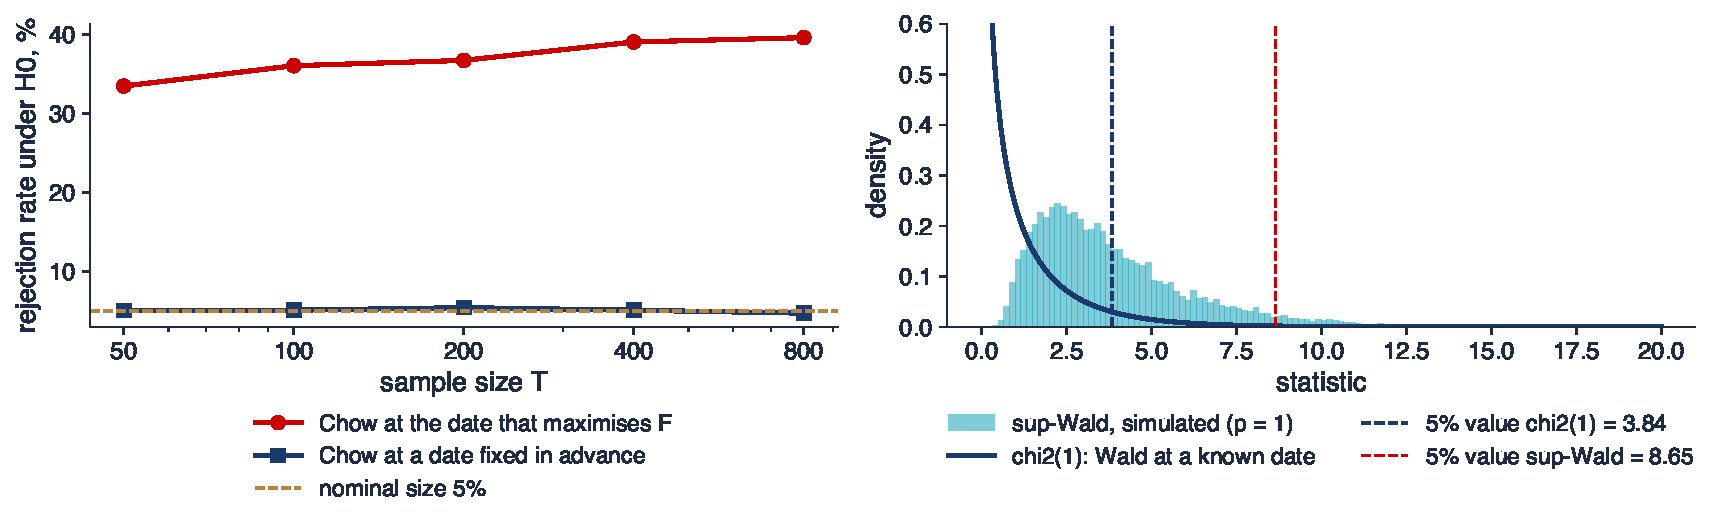
\includegraphics[width=0.97\textwidth,height=0.52\textheight,keepaspectratio]{ats_ch2_chow_snooping.pdf}
\end{center}
\vspace{-0.25cm}
\begin{itemize}
    \item Stînga: zgomot alb, testul Chow pentru o schimbare de medie la 5\%, 4\,000 de replicări pentru fiecare $T$; dreapta: densitatea simulată sub $H_0$ a lui $\sup_\pi W_T(\pi)$, $\pi \in [0{,}15; 0{,}85]$, față de $\chi^2(1)$
\end{itemize}
\quantlet{ATS\_ch2\_chow\_snooping}{\qlurl{ATS_ch2_chow_snooping}}
\end{frame}

\begin{frame}{Interpretarea distorsiunii de mărime}
\itemsize{\small}
\begin{itemize}
    \item La o dată fixată dinainte testul își păstrează mărimea (5{,}1\% pentru $T = 100$); la data care maximizează statistica respinge o ipoteză nulă adevărată în 33\% pînă la 40\% din eșantioane
    \begin{itemize}
        \item distorsiunea crește lent cu $T$: mai multe date candidate, un maxim mai mare
    \end{itemize}
    \item Valoarea critică de 5\% a supremumului este 8{,}65, față de 3,84 pentru $\chi^2(1)$; cu doi coeficienți 11{,}69
    \item Lecția: căutarea datei face parte din test; valorile critice trebuie să țină cont de ea
\end{itemize}
\end{frame}

\begin{frame}{Recapitulare: instabilitatea și datele cunoscute}
\itemsize{\small}
\begin{itemize}
    \item O ruptură este o schimbare a lui $\beta_t$; totală sau parțială, în medie, în dinamică sau în varianță
    \item Chow: un test $F$ valid doar pentru o dată fixată înainte de a vedea datele
    \item Alegerea datei din date multiplică de cîteva ori mărimea testului
    \item Data rupturii este un parametru neidentificat sub $H_0$
\end{itemize}
\end{frame}


%=============================================================================
\section{O ruptură la o dată necunoscută}
%=============================================================================

\begin{frame}{Testul sup-Wald al lui Andrews (1993) (1/2)}
\itemsize{\small}
\begin{itemize}
    \item Calculăm statistica Chow--Wald $W_T(\pi)$ pentru fiecare fracție candidată a rupturii și o luăm pe cea mai mare \refAnd
    \begin{itemize}
        \item $\sup_{\pi \in \Pi} W_T(\pi)$, $\quad \Pi = [\pi_0, 1 - \pi_0]$
        \item $\Pi$: fracțiile candidate; $\pi_0$: \textbf{trunchierea}, de obicei 0,15, astfel încît fiecare regim să aibă cel puțin 15\% din eșantion
        \item variantele LM, Wald și LR au aceeași limită; \refQua\ a folosit varianta LR
    \end{itemize}
    \item \textbf{Teoremă} \refAnd: sub $H_0$ și în condiții de regularitate (regresori staționari, cu dependență slabă)
    \begin{itemize}
        \item $W_T(\cdot) \Rightarrow Q_p(\pi) = \dfrac{\|B_p(\pi) - \pi B_p(1)\|^2}{\pi(1 - \pi)}$
        \item $\Rightarrow$: convergența întregului proces în $\pi$; $B_p$: o mișcare browniană standard $p$-dimensională; $p$: numărul coeficienților care se pot schimba
        \item $B_p(\pi) - \pi B_p(1)$ este o punte browniană; $\pi(1 - \pi)$ este varianța ei: $Q_p(\pi)$ este o punte la pătrat, standardizată (\atsapplink{atsapp1}{atssrc1}{Anexă})
    \end{itemize}
\end{itemize}
\end{frame}

\begin{frame}{Testul sup-Wald al lui Andrews (1993) (2/2)}
\itemsize{\small}
\begin{itemize}
    \item Limita: $\sup W_T \to_d \sup_{\pi \in \Pi} Q_p(\pi)$
    \begin{itemize}
        \item la un $\pi$ fixat, $Q_p(\pi) \sim \chi^2(p)$; supremumul peste multe valori $\pi$ este mult mai mare
    \end{itemize}
    \item De ce este necesară trunchierea: $\sup_{\pi \in (0,1)} Q_p(\pi) = \infty$ aproape sigur (legea logaritmului iterat)
    \begin{itemize}
        \item valorile critice depind de $p$ și $\pi_0$; aici simulate: $p = 1$: 7{,}11 (10\%), 8{,}65 (5\%), 12{,}17 (1\%)
    \end{itemize}
\end{itemize}
\end{frame}

\begin{frame}{Teste optime: Andrews și Ploberger (1994)}
\itemsize{\small}
\begin{itemize}
    \item Supremumul nu este singura funcțională; medierea este optimă împotriva alternativelor apropiate de $H_0$ \refAP
    \begin{itemize}
        \item $|\Pi| = 1 - 2\pi_0$: lungimea mulțimii fracțiilor candidate; ambele statistici mediază peste ea
        \item $\mathrm{expW} = \ln\Big(\dfrac{1}{|\Pi|}\displaystyle\int_\Pi \exp\big(\tfrac12 W_T(\pi)\big)d\pi\Big)$: putere medie ponderată, pentru rupturi medii și mari
        \item $\mathrm{aveW} = \dfrac{1}{|\Pi|}\displaystyle\int_\Pi W_T(\pi)\,d\pi$: optim pentru rupturi foarte mici, apropiat de testul Nyblom pentru coeficienți de tip mers aleator
    \end{itemize}
    \item Valori de 5\% pentru $p = 1$, $\pi_0 = 0{,}15$ (simulate): sup 8{,}65, exp 2{,}02, ave 2{,}87
    \item Testul sup-Wald are putere împotriva \emph{oricărui} tip de instabilitate, nu doar a unei singure rupturi
    \begin{itemize}
        \item o respingere spune „instabil”, nu „o ruptură la $\hat\pi$”; numărul rupturilor este subiectul secțiunii 3
    \end{itemize}
\end{itemize}
\end{frame}

\begin{frame}{Estimarea datei rupturii (1/2)}
\itemsize{\small}
\begin{itemize}
    \item Cele mai mici pătrate: alegem data care minimizează SSR total al celor două regimuri
    \begin{itemize}
        \item $\hat T_1 = \arg\min_{T_1} [S_1(T_1) + S_2(T_1)]$
        \item $S_1(T_1)$, $S_2(T_1)$: SSR înainte și după o dată candidată $T_1$; echivalent cu data celei mai mari statistici Wald sub homoscedasticitate
    \end{itemize}
    \item Precizia \refBai
    \begin{itemize}
        \item pentru o ruptură de mărime fixă, $\hat T_1 - T_1 = O_p(1)$: eroarea \textbf{datei} este mărginită în probabilitate și nu crește cu $T$
        \item deci fracția $\hat\pi = \hat T_1/T$ converge cu rata $T$, mai repede decît rata obișnuită $\sqrt T$
        \item coeficienții regimurilor sînt $\sqrt T$-consistenți și asimptotic Normali ca și cum data ar fi cunoscută
    \end{itemize}
\end{itemize}
\end{frame}

\begin{frame}{Estimarea datei rupturii (2/2)}
\itemsize{\small}
\begin{itemize}
    \item Interval de încredere pentru dată \refBai: cu o ruptură care scade, $\Delta_T \to 0$
    \begin{itemize}
        \item $\Delta_T^2\sigma^{-2}(\hat T_1 - T_1) \to_d \arg\max_s Z(s)$, $\quad Z(s) = W(s) - |s|/2$
        \item $\Delta_T$: mărimea schimbării mediei; $\sigma^2$: varianța erorii; $W(s)$: o mișcare browniană bilaterală, $s \in \mathbb R$
        \item intervalul este data $\pm$ cuantile ale lui $\arg\max Z$, rescalate cu $\sigma^2/\hat\Delta^2$
    \end{itemize}
    \item Interpretare
    \begin{itemize}
        \item rupturi mari, zgomot mic: interval scurt; intervalul este asimetric cînd varianțele diferă între regimuri
    \end{itemize}
\end{itemize}
\end{frame}

\begin{frame}{Studiu de caz: McConnell și Perez-Quiros (2000)}
\itemsize{\footnotesize}
\begin{columns}[T]
\begin{column}{0.36\textwidth}
\centering
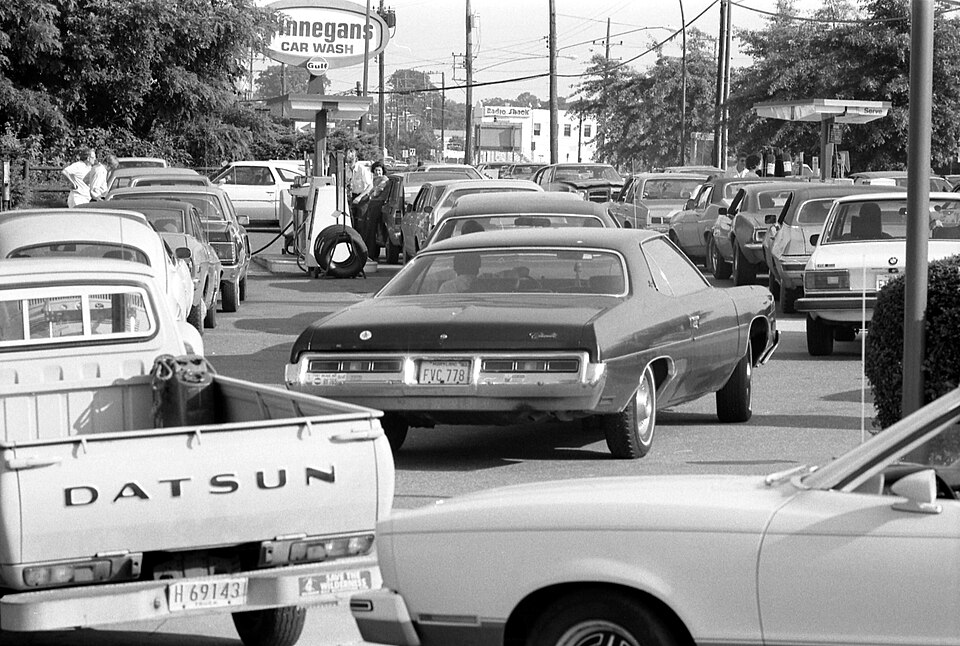
\includegraphics[height=0.36\textheight]{ch2_gasline_1979.jpg}\\[1mm]
\imgcap{Coadă la benzină, Maryland, 15 iunie 1979}
\imgcredit{https://commons.wikimedia.org/wiki/File:Line_at_a_gas_station,_June_15,_1979.jpg}{Foto: Warren K. Leffler (1979), Library of Congress; domeniu public; Wikimedia Commons}
\end{column}
\begin{column}{0.62\textwidth}
\begin{itemize}
    \item Lucrarea: creșterea PIB real în SUA, T2 1953--T2 1999; AR(1) pentru media condiționată; apoi o ruptură în media lui $\sqrt{\pi/2}\,|\hat e_t|$, o estimare nedeplasată a abaterii standard sub distribuția Normală \refMPQ
    \begin{itemize}
        \item $\hat e_t$: reziduul AR(1); aici $\pi = 3{,}14\ldots$; dacă $e_t \sim N(0, \sigma^2)$, $\E|e_t| = \sigma\sqrt{2/\pi}$, de unde factorul
        \item teste: sup-, exp-, ave-Wald \refAnd, \refAP; rezultatul lor: o ruptură în varianță în T1 1984, „Marea Moderație” (Great Moderation)
    \end{itemize}
    \item Replicarea noastră: aceiași doi pași pe FRED GDPC1 (versiunea de azi), statistici Wald robuste, p-value-uri simulate; apoi eșantionul extins pînă în 2026
    \item Întrebarea: se menține ruptura în varianță pe datele revizuite și după trimestrele COVID-19?
\end{itemize}
\end{column}
\end{columns}
\end{frame}

\begin{frame}{Marea Moderație în creșterea PIB din SUA}
\itemsize{\footnotesize}
\begin{center}
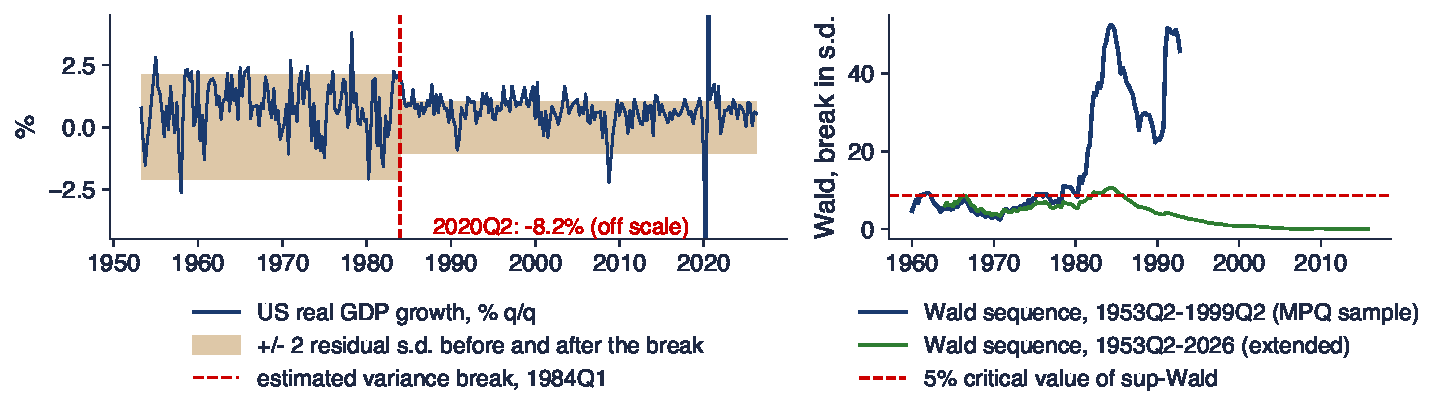
\includegraphics[width=0.97\textwidth,height=0.64\textheight,keepaspectratio]{ats_ch2_great_moderation.pdf}
\end{center}
\vspace{-0.25cm}
\begin{itemize}
    \item Sus: creșterea cu $\pm 2$ abateri standard reziduale înainte și după ruptura estimată; jos: șirul statisticilor Wald pentru o ruptură în $\E\sqrt{\pi/2}|e_t|$ (HAC), două eșantioane
\end{itemize}
\quantlet{ATS\_ch2\_great\_moderation}{\qlurl{ATS_ch2_great_moderation}}
\end{frame}

\begin{frame}{Interpretarea rupturii în varianță}
\itemsize{\small}
\begin{itemize}
    \item Eșantionul MPQ ($T = 185$): sup-Wald 52{,}5 ($p$ $<$\,0{,}001), exp 23{,}2, ave 17{,}5; data T1 1984, aceeași cu cea găsită de \refMPQ
    \begin{itemize}
        \item abaterea standard reziduală 1{,}06 înainte, 0{,}45 după: varianța scade de 5{,}5 ori; nicio ruptură în ecuația mediei (sup 3{,}2, $p$ 0{,}861)
    \end{itemize}
    \item Pînă în 2019: ruptura se mută cu un trimestru (T2 1984), raportul varianțelor 4{,}1; Marea Moderație s-a menținut și după recesiunea din 2008--2009
    \item Pînă în 2026: sup-Wald scade la 10{,}7 ($p$ 0{,}019) și raportul la 1{,}1: două valori extreme (T2 2020: \ensuremath{-}8{,}2\%) domină varianța de după ruptură
    \begin{itemize}
        \item o a doua ruptură sau valori extreme? Un test cu o singură ruptură nu poate decide; sînt necesari estimatori robuști ai scalei sau o a doua ruptură
    \end{itemize}
\end{itemize}
\end{frame}

\begin{frame}{Recapitulare: o ruptură la o dată necunoscută}
\itemsize{\small}
\begin{itemize}
    \item sup-Wald: supremumul unei punți browniene la pătrat; trunchiați și folosiți valorile critice proprii
    \item exp- și ave-Wald sînt optime pentru rupturi moderate și mici
    \item Data se estimează precis, intervalul de încredere vine din $\arg\max_s\{W(s) - |s|/2\}$
    \item Rupturile în varianță: testați media lui $|\hat e_t|$; valorile extreme le pot ascunde sau imita
\end{itemize}
\end{frame}


%=============================================================================
\section{Rupturi multiple: Bai și Perron}
%=============================================================================

\begin{frame}{Modelul cu rupturi multiple}
\itemsize{\small}
\begin{itemize}
    \item $y_t = x_t'\beta + z_t'\delta_j + u_t$, $t = T_{j-1} + 1, \dots, T_j$, $j = 1, \dots, m + 1$, cu $T_0 = 0$, $T_{m+1} = T$ \refBPa
    \begin{itemize}
        \item $T_1 < \dots < T_m$: datele rupturilor; $\delta_j$: coeficienții lui $z_t$ în regimul $j$; $\beta$: cei ai lui $x_t$, comuni tuturor regimurilor
        \item schimbare totală: fără $x_t$; modelul cu schimbări de medie: $z_t = 1$
        \item lungimea minimă a unui segment $h = [\varepsilon T]$, de obicei $\varepsilon = 0{,}15$; erorile pot fi autocorelate și heteroscedastice între regimuri
    \end{itemize}
    \item Estimatorul: minimul \textbf{global} al SSR peste toate partițiile admisibile $(T_1, \dots, T_m)$
    \begin{itemize}
        \item fracțiile rupturilor sînt consistente cu rata $T$, ca pentru o ruptură; datele se estimează împreună, nu una cîte una
    \end{itemize}
    \item Forța brută cere $O(T^m)$ regresii; programarea dinamică cere $O(T^2)$ \refBPb
\end{itemize}
\end{frame}

\begin{frame}{Programarea dinamică}
\itemsize{\small}
\begin{itemize}
    \item Pasul 1: calculăm $\mathrm{SSR}(i, j)$ al unei regresii pe fiecare segment $[i, j]$ cu $j - i + 1 \ge h$ (reziduuri recursive: $O(T^2)$ operații)
    \item Pasul 2: recursia Bellman pentru cea mai bună partiție cu $r$ rupturi a primelor $n$ observații
    \begin{itemize}
        \item $\mathrm{SSR}(\{T_{r,n}\}) = \min_{rh \le j \le n - h}\big[\mathrm{SSR}(\{T_{r-1,j}\}) + \mathrm{SSR}(j + 1, n)\big]$
        \item $\{T_{r,n}\}$: cea mai bună partiție a observațiilor $1, \dots, n$ cu $r$ rupturi; $j$: data ultimei ei rupturi; $h$: lungimea minimă a unui segment
        \item partiția optimă cu $m$ rupturi conține partiții optime ale prefixelor ei (principiul lui Bellman)
    \end{itemize}
    \item O singură trecere dă partițiile optime pentru orice $m \le M$: datele de intrare ale tuturor testelor și criteriilor
    \begin{itemize}
        \item schimbarea parțială ($\beta$ comun) cere o iterație între $\beta$ și partiție \refBPb; Seminarul 2, A3 parcurge recursia de mînă
    \end{itemize}
\end{itemize}
\end{frame}

\begin{frame}{Testarea și alegerea numărului de rupturi (1/2)}
\itemsize{\small}
\begin{itemize}
    \item $\sup F_T(k)$: nicio ruptură față de exact $k$ rupturi, la partiția optimă după SSR, cu varianță robustă \refBPa
    \begin{itemize}
        \item $M$: numărul maxim de rupturi luat în calcul (aici 5)
        \item \textbf{UDmax} $= \max_{k \le M}\sup F_T(k)$: nicio ruptură față de un număr necunoscut de rupturi, cel mult $M$
        \item \textbf{WDmax}: la fel, cu fiecare $k$ ponderat prin raportul valorilor critice
    \end{itemize}
    \item Testul \textbf{secvențial} $\sup F_T(\ell + 1 \mid \ell)$: $\ell$ rupturi față de $\ell + 1$
    \begin{itemize}
        \item pentru fiecare dintre cele $\ell + 1$ segmente, cea mai mare statistică pentru o ruptură; adăugăm o ruptură cît timp testul respinge
        \item strategia recomandată \refBPb: întîi UDmax sau WDmax, apoi testele secvențiale
    \end{itemize}
\end{itemize}
\end{frame}

\begin{frame}{Testarea și alegerea numărului de rupturi (2/2)}
\itemsize{\small}
\begin{itemize}
    \item Criterii informaționale: alegem $m$ cu cea mai mică valoare
    \begin{itemize}
        \item $\mathrm{BIC}(m) = \ln(\mathrm{SSR}_m/T) + p^*\ln T/T$
        \item \textbf{LWZ}: $\ln\frac{\mathrm{SSR}_m}{T - p^*} + p^*\frac{0{,}299}{T}(\ln T)^{2{,}1}$ \refLWZ
        \item $\mathrm{SSR}_m$: SSR al celei mai bune partiții cu $m$ rupturi; $p^*$: numărul coeficienților și al datelor rupturilor; al doilea termen penalizează rupturile suplimentare
    \end{itemize}
    \item Slăbiciuni cunoscute
    \begin{itemize}
        \item BIC alege prea multe rupturi cu autocorelație, LWZ prea puține cu rupturi mici
    \end{itemize}
\end{itemize}
\end{frame}

\begin{frame}{Studiu de caz: Bai și Perron (2003), rata reală a dobînzii în SUA}
\itemsize{\footnotesize}
\begin{columns}[T]
\begin{column}{0.36\textwidth}
\centering

\includegraphics[height=0.33\textheight]{ch2_volcker_reagan_1981.jpg}\\[1mm]
\imgcap{Paul Volcker (stînga) și Ronald Reagan, decembrie 1981}
\imgcredit{https://commons.wikimedia.org/wiki/File:President_Ronald_Reagan_Paul_Volcker_Meeting_to_Discuss_Monetary_Policy_with_Paul_Volker_in_Oval_Office_-_DPLA_-_e04117f4897610a724c267cdf855ce73.jpg}{Foto: White House Photographic Office (1981); domeniu public; Wikimedia Commons}
\end{column}
\begin{column}{0.62\textwidth}
\begin{itemize}
    \item Lucrarea, secțiunea 6.1: rata reală ex post din \refGP, trimestrial T1 1961--T3 1986 ($T = 103$), model cu schimbări de medie, $\varepsilon = 0{,}15$ ($h = 15$), $M = 5$, varianțe HAC diferite între segmente \refBPb
    \begin{itemize}
        \item replicarea noastră folosește fișierul lor de date (arhiva de date JAE) și aceleași setări
    \end{itemize}
    \item Extensie: seria reconstruită din FRED (dobînda la titlurile de stat la sfîrșitul trimestrului minus inflația IPC din trimestrul următor), corelație 0{,}99 cu originalul, T1 1961--T1 2026
    \item Întrebarea: cîte regimuri și corespund ele istoriei politicii monetare?
\end{itemize}
\end{column}
\end{columns}
\end{frame}

\begin{frame}{Schimbări de medie în rata reală a dobînzii din SUA}
\itemsize{\footnotesize}
\begin{center}
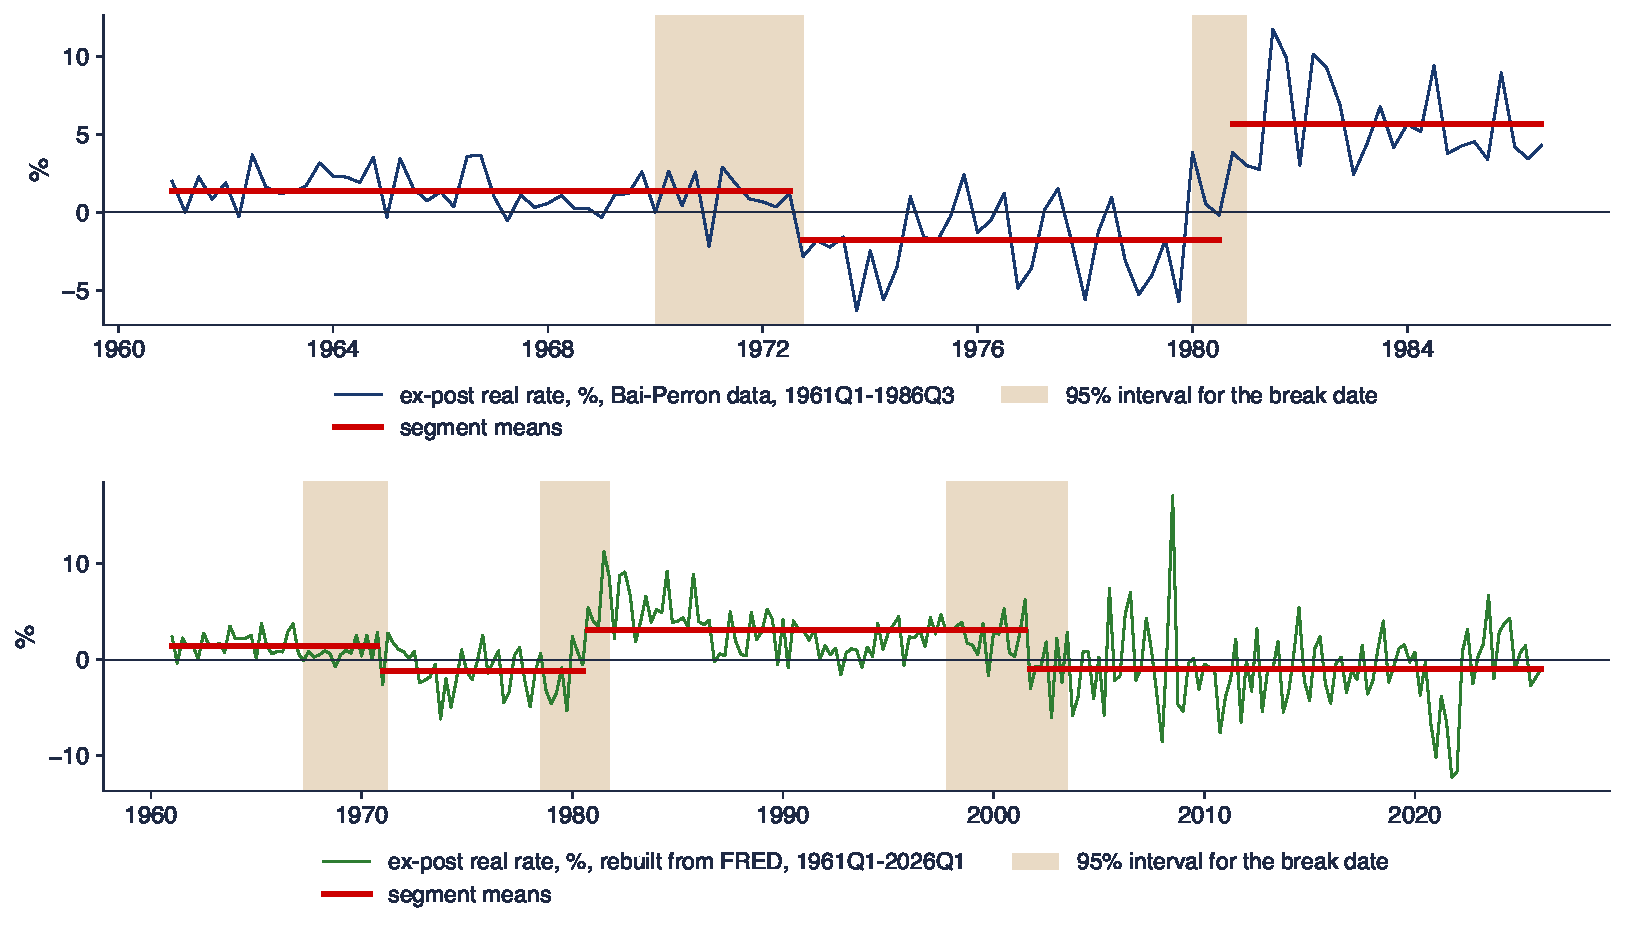
\includegraphics[width=0.97\textwidth,height=0.64\textheight,keepaspectratio]{ats_ch2_bai_perron.pdf}
\end{center}
\vspace{-0.25cm}
\begin{itemize}
    \item Roșu: mediile segmentelor partiției alese de BIC/LWZ; umbrit: intervale de 95\% pentru date \refBai, varianțe de termen lung diferite. Sus: datele originale; jos: reconstruite pînă în 2026
\end{itemize}
\quantlet{ATS\_ch2\_bai\_perron}{\qlurl{ATS_ch2_bai_perron}}
\end{frame}

\begin{frame}{Interpretarea rezultatelor Bai--Perron}
\itemsize{\footnotesize}
\begin{center}
\scriptsize
\begin{tabular}{lrrrrrr}
\toprule
\textbf{$m$} & 0 & 1 & 2 & 3 & 4 & 5 \\
\midrule
SSR & 1215 & 645 & 456 & 445 & -- & -- \\
$\sup F_T(m)$ & -- & 61{,}1 & 46{,}1 & 36{,}1 & 27{,}4 & 20{,}6 \\
valoarea de 5\% & -- & 8{,}74 & 7{,}27 & 6{,}05 & -- & -- \\
BIC & 2{,}513 & 1{,}970 & 1{,}713 & 1{,}779 & -- & -- \\
LWZ & 2{,}550 & 2{,}082 & 1{,}901 & 2{,}043 & -- & -- \\
\bottomrule
\end{tabular}
\end{center}
\begin{itemize}
    \item UDmax 61{,}1 (5\%: 8{,}87); secvențial: $F(2|1) = 36{,}9$, $F(3|2) = 16{,}1$, $F(4|3) = 0{,}04$ (5\%: 10{,}54; 11{,}56): 3 rupturi, T4 1966, T3 1972, T3 1980
    \begin{itemize}
        \item BIC și LWZ aleg 2 rupturi: T3 1972, T3 1980; datele sînt cele raportate de \refBPb
    \end{itemize}
    \item Mediile 1{,}36\%, \ensuremath{-}1{,}80\%, 5{,}64\%: rate reale negative în anii 1970, apoi dezinflația din 1979--1981; intervale de 95\% [T1 1970; T4 1972], [T1 1980; T1 1981]
    \item Eșantionul extins: 3 rupturi (T4 1970, T3 1980, T3 2001); ultimul regim are media \ensuremath{-}0{,}97\%: era dobînzilor mici de după 2001, intervalul [T4 1997; T3 2003]
\end{itemize}
\end{frame}

\begin{frame}{Schimbări de medie în inflația din România}
\itemsize{\footnotesize}
\begin{center}
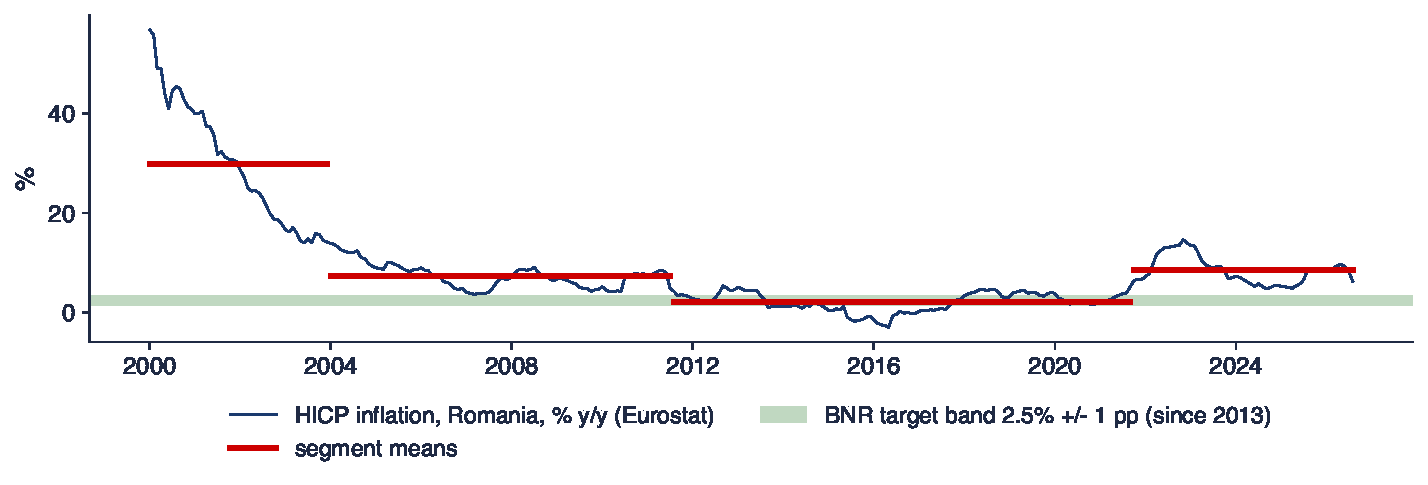
\includegraphics[width=0.97\textwidth,height=0.48\textheight,keepaspectratio]{ats_ch2_ro_inflation_breaks.pdf}
\end{center}
\vspace{-0.25cm}
\begin{itemize}
    \item Inflația IAPC, anuală, ianuarie 2000--august 2026 ($T = 320$), schimbări de medie Bai--Perron, $\varepsilon = 0{,}15$, $M = 5$; roșu: partiția aleasă de BIC și LWZ
\end{itemize}
\quantlet{ATS\_ch2\_ro\_inflation\_breaks}{\qlurl{ATS_ch2_ro_inflation_breaks}}
\end{frame}

\begin{frame}{Interpretarea regimurilor inflației din România}
\itemsize{\small}
\begin{itemize}
    \item BIC și LWZ: 3 rupturi (decembrie 2003, iulie 2011, septembrie 2021); mediile 29{,}8\%, 7{,}5\%, 2{,}2\%, 8{,}5\%
    \begin{itemize}
        \item dezinflația, țintirea inflației (adoptată în august 2005), deceniul inflației scăzute, valul inflaționist din 2021--2023
    \end{itemize}
    \item Procedura secvențială robustă se oprește la 1 ruptură: $\sup F(1) = 12{,}8$, dar $F(2|1) = 2{,}06$
    \begin{itemize}
        \item inflația este foarte persistentă în interiorul regimurilor: varianța HAC absoarbe schimbările, iar testul își pierde puterea
        \item din același motiv, intervalele de 95\% pentru date acoperă ani întregi (a doua dată: [ianuarie 2000; decembrie 2014]); nu sînt desenate
    \end{itemize}
    \item Un model mai bun: schimbare parțială în termenul liber al unui model AR, astfel încît erorile să fie aproape de zgomot alb (idee de proiect)
\end{itemize}
\end{frame}

\begin{frame}{Detectarea punctelor de schimbare în statistică și machine learning}
\itemsize{\small}
\begin{itemize}
    \item Segmentare penalizată: minimizăm $\sum_j \mathrm{cost}(\text{segmentul } j) + \beta\,m$ după partiții
    \begin{itemize}
        \item $\mathrm{cost}$: de exemplu SSR sau minus log-verosimilitatea unui segment; $\beta > 0$: penalizarea pentru fiecare ruptură; $m$: numărul rupturilor
        \item PELT reduce recursia Bellman la $O(T)$ în condiții slabe \refKFE; segmentarea binară și segmentarea binară aleatoare (wild binary segmentation) \refFry\ funcționează pe serii lungi
        \item pachetul Python \texttt{ruptures} le conține \refTOV; BIC-ul din Bai--Perron este o penalizare particulară
    \end{itemize}
    \item Ce adaugă econometria: inferența pentru numărul rupturilor și intervale de încredere pentru date cu autocorelație
    \begin{itemize}
        \item rupturi comune în sisteme de ecuații \refOP; sinteză \refCP
    \end{itemize}
    \item Practica inginerească ajustează penalizarea pe date etichetate; econometria fixează mărimea unui test: ambele sînt valide dacă alegerea este preînregistrată
\end{itemize}
\end{frame}

\begin{frame}{Recapitulare: rupturi multiple}
\itemsize{\small}
\begin{itemize}
    \item Cele mai mici pătrate globale peste toate partițiile, prin programare dinamică în $O(T^2)$
    \item UDmax/WDmax, apoi $F(\ell + 1|\ell)$ secvențial; BIC și LWZ ca verificare
    \item Rata reală din SUA: rupturile din T3 1972 și T3 1980 replicate; încă un regim după 2001
    \item Erori persistente: testele robuste își pierd puterea, iar intervalele pentru date devin largi
\end{itemize}
\end{frame}


%=============================================================================
\section{Teste de fluctuație și monitorizare în timp real}
%=============================================================================

\begin{frame}{Testele CUSUM și MOSUM (1/2)}
\itemsize{\small}
\begin{itemize}
    \item Reziduurile recursive \refBDE: eroarea de prognoză pe un pas, standardizată, a modelului estimat pînă la $t - 1$
    \begin{itemize}
        \item $w_t = (y_t - x_t'\hat\beta_{t-1})/\sqrt{1 + x_t'(X_{t-1}'X_{t-1})^{-1}x_t}$
        \item $\hat\beta_{t-1}$: MCMMP pe observațiile $1, \dots, t - 1$; $X_{t-1}$: matricea regresorilor lor; radicalul corectează pentru incertitudinea estimării
        \item sub $H_0$ și cu erori Normale, $w_t$ sînt i.i.d.\ $N(0, \sigma^2)$
    \end{itemize}
    \item CUSUM: suma cumulată a reziduurilor recursive standardizate
    \begin{itemize}
        \item $W_r = \hat\sigma^{-1}\sum_{t = k+1}^{r} w_t$, frontiera de 5\% $\pm 0{,}948[\sqrt{T - k} + 2(r - k)/\sqrt{T - k}]$
        \item $k$: numărul regresorilor (primele $k$ observații pornesc recursia); $W_r$ se comportă ca o mișcare browniană; depășirea frontierei semnalează o ruptură
    \end{itemize}
\end{itemize}
\end{frame}

\begin{frame}{Testele CUSUM și MOSUM (2/2)}
\itemsize{\small}
\begin{itemize}
    \item Ce detectează CUSUM
    \begin{itemize}
        \item schimbări în termenul liber și o derivă sistematică a erorilor de prognoză; slab împotriva schimbărilor care se compensează
    \end{itemize}
    \item OLS-CUSUM folosește reziduurile obișnuite: limita este o punte browniană \refPK; MOSUM însumează pe o fereastră mobilă de lățime fixă \refCHK
    \begin{itemize}
        \item MOSUM reacționează mai repede la o ruptură în mijlocul eșantionului și la schimbări temporare
    \end{itemize}
    \item Acestea sînt teste \textbf{retrospective}: întregul eșantion este disponibil cînd se aplică testul
\end{itemize}
\end{frame}

\begin{frame}{Monitorizarea: eșecul testelor repetate (1/2)}
\itemsize{\small}
\begin{itemize}
    \item O bancă centrală estimează un model pe $m$ observații istorice și întreabă, la fiecare nouă publicare, „s-a stricat?”
    \begin{itemize}
        \item un test de 5\% repetat la $n = m + 1, m + 2, \dots$ respinge pînă la urmă o ipoteză nulă adevărată cu probabilitatea 1: legea logaritmului iterat
    \end{itemize}
    \item \refCSW: monitorizăm CUSUM al noilor reziduuri recursive și ne oprim prima dată cînd depășește o frontieră care se lărgește
    \begin{itemize}
        \item $Q_n = \hat\sigma^{-1}\sum_{t = m+1}^{n} w_t$, $\quad$ alarmă dacă $|Q_n| > \sqrt{n\,[a^2 + \ln(n/m)]}$
        \item $n$: dimensiunea curentă a eșantionului; $a$: o constantă aleasă pentru a fixa probabilitatea unei alarme false; termenul $\ln(n/m)$ lărgește frontiera pe măsură ce trece timpul
    \end{itemize}
\end{itemize}
\end{frame}

\begin{frame}{Monitorizarea: eșecul testelor repetate (2/2)}
\itemsize{\small}
\begin{itemize}
    \item Frontiera vine din \refRS:
    \begin{itemize}
        \item $P\{\exists u \ge 1: |W(u) - W(1)| \ge \sqrt{u(a^2 + \ln u)}\} = 2[1 - \Phi(a) + a\varphi(a)]$
        \item $W$: o mișcare browniană standard; $u = n/m$; $\Phi$, $\varphi$: funcția de repartiție și densitatea distribuției Normale standard
        \item $a^2 = 7{,}78$: mărimea 5{,}1\% pe un orizont \emph{infinit}; $a^2 = 6{,}25$: 10{,}0\%
    \end{itemize}
    \item Monitorizarea pe baza prognozelor: eșecul prognozelor \refGRa\ și testul de fluctuație al acurateței relative \refGRb\ (\atschlink{https://danpele.github.io/Advanced-Time-Series/RO/Cursuri/capitol1_evaluarea_prognozelor.pdf}{Capitolul 1})
\end{itemize}
\end{frame}

\begin{frame}{Alarme false și monitorizarea în timp real a inflației din România}
\itemsize{\footnotesize}
\begin{center}
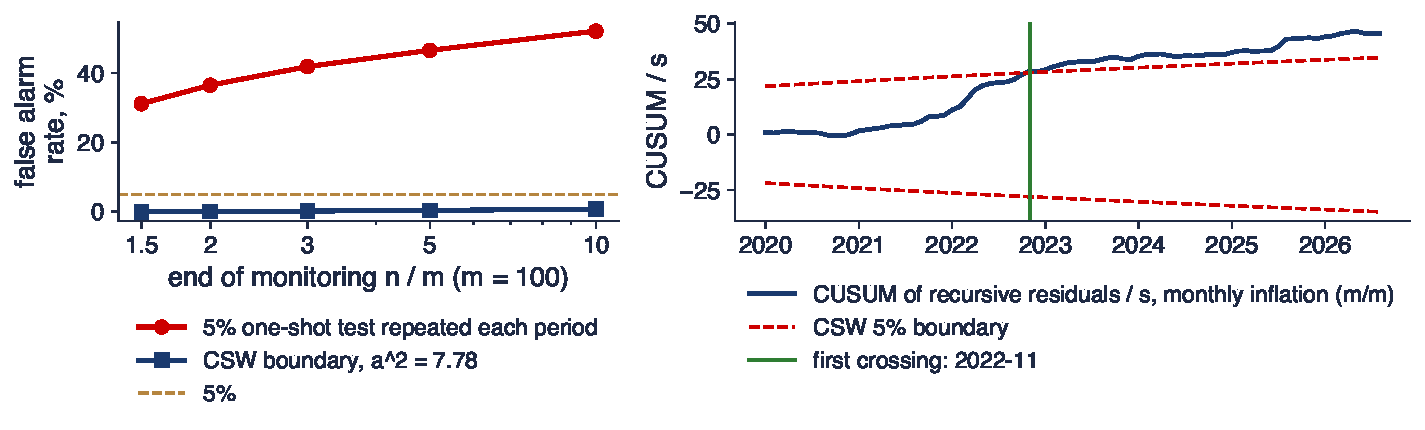
\includegraphics[width=0.97\textwidth,height=0.5\textheight,keepaspectratio]{ats_ch2_monitoring.pdf}
\end{center}
\vspace{-0.25cm}
\begin{itemize}
    \item Stînga: zgomot alb, $m = 100$, 2\,000 de replicări; dreapta: media inflației IAPC lunare, eșantion istoric 2015--2019, monitorizare din ianuarie 2020
\end{itemize}
\quantlet{ATS\_ch2\_monitoring}{\qlurl{ATS_ch2_monitoring}}
\end{frame}

\begin{frame}{Interpretarea rezultatelor monitorizării}
\itemsize{\small}
\begin{itemize}
    \item Testele de 5\% repetate dau o alarmă falsă în 36\% din eșantioane pînă la $n = 2m$ și în 52\% pînă la $n = 10m$; frontiera CSW în 0{,}8\%
    \begin{itemize}
        \item mărimea CSW se atinge doar cînd $n \to \infty$: pe un orizont finit frontiera este conservatoare
    \end{itemize}
    \item România: media istorică 0{,}15\% pe lună, $\hat\sigma = 0{,}51$; CUSUM trece de frontieră în noiembrie 2022
    \begin{itemize}
        \item testul naiv repetat ar fi semnalat în ianuarie 2022; cu $\hat\sigma$ de termen lung (HAC) semnalul vine abia în august 2025
    \end{itemize}
    \item Prețul unei rate controlate a alarmelor false este întîrzierea: aproape doi ani după ce inflația a început să crească, în 2021
\end{itemize}
\end{frame}

\begin{frame}{Recapitulare: monitorizarea}
\itemsize{\small}
\begin{itemize}
    \item CUSUM și MOSUM ale reziduurilor recursive: teste de fluctuație retrospective
    \item Repetarea unui test unic pe măsură ce sosesc datele garantează o alarmă falsă
    \item Frontiera CSW $\sqrt{n[a^2 + \ln(n/m)]}$ controlează mărimea pe un orizont infinit
    \item Inflația din România: detectare la sfîrșitul lui 2022, o întîrziere lungă, dar cu rata alarmelor false controlată
\end{itemize}
\end{frame}


%=============================================================================
\section{Rupturi în varianță}
%=============================================================================

\begin{frame}{Algoritmul ICSS și corecția lui (1/2)}
\itemsize{\small}
\begin{itemize}
    \item \refIT: comparăm suma cumulată a pătratelor cu o dreaptă
    \begin{itemize}
        \item $C_k = \sum_{t \le k} a_t^2$, $\quad D_k = C_k/C_T - k/T$, $\quad \mathrm{IT} = \sqrt{T/2}\max_k|D_k| \Rightarrow \sup|B^0(r)|$
        \item $a_t$: randamentele centrate; $C_k/C_T$: proporția din suma totală a pătratelor atinsă la $k$; cu varianță constantă ea crește ca $k/T$
        \item $B^0$: o punte browniană pe $[0,1]$; valoarea critică de 5\% este 1,358; data este valoarea $k$ cu cel mai mare $|D_k|$
    \end{itemize}
    \item ICSS (sume cumulate de pătrate, iterate)
    \begin{itemize}
        \item aplicăm testul iterativ pe subsegmente (segmentare binară), apoi reverificăm fiecare ruptură între vecinele ei
    \end{itemize}
\end{itemize}
\end{frame}

\begin{frame}{Algoritmul ICSS și corecția lui (2/2)}
\itemsize{\small}
\begin{itemize}
    \item Factorul $\sqrt{T/2}$ presupune $\Var(a_t^2) = 2\sigma^4$: date i.i.d.\ Normale
    \begin{itemize}
        \item cu coeficientul de boltire $\kappa = \E a_t^4/\sigma^4$, statistica este mărită artificial de $\sqrt{(\kappa - 1)/2}$ ori; cu GARCH, $a_t^2$ este și autocorelat
    \end{itemize}
    \item $\kappa_2$ din \refSAC: același CUSUM, scalat printr-o varianță de termen lung
    \begin{itemize}
        \item $\kappa_2 = \max_k|C_k - (k/T)C_T|/\sqrt{T\hat\omega_4}$
        \item $\hat\omega_4$: varianța de termen lung a lui $a_t^2 - \hat\sigma^2$ (nucleul Bartlett, \atschlink{https://danpele.github.io/Advanced-Time-Series/RO/Cursuri/capitol0_recapitulare_inferenta.pdf}{Capitolul 0})
        \item aceeași limită, validă cu cozi groase și heteroscedasticitate condiționată
    \end{itemize}
\end{itemize}
\end{frame}

\begin{frame}{Regimuri de varianță pentru EUR/RON}
\itemsize{\footnotesize}
\begin{center}
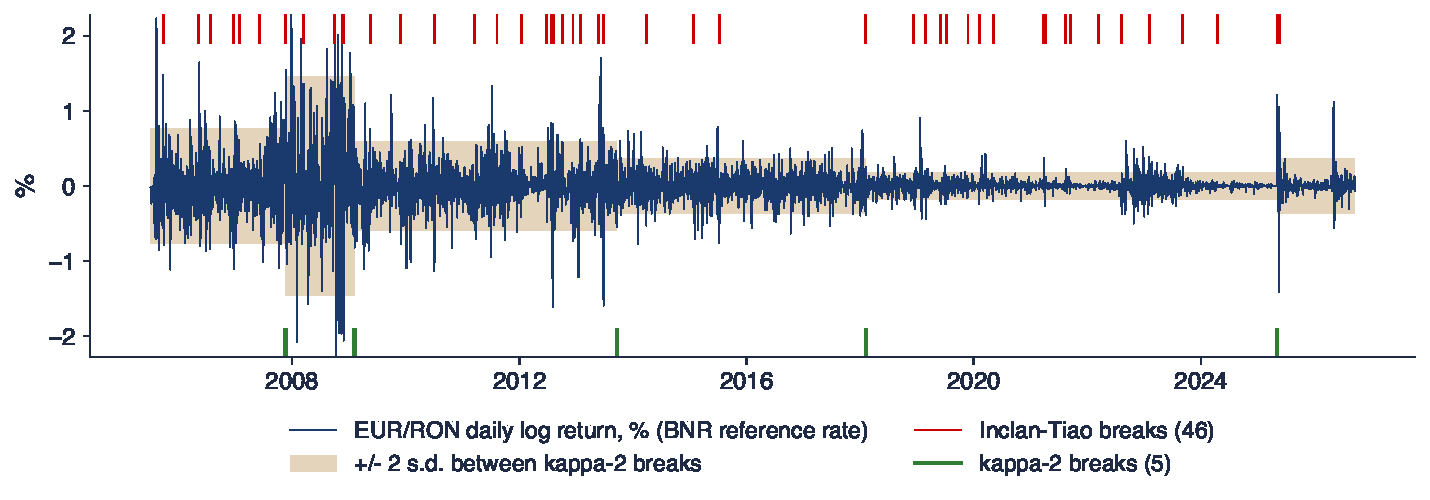
\includegraphics[width=0.97\textwidth,height=0.5\textheight,keepaspectratio]{ats_ch2_variance_breaks.pdf}
\end{center}
\vspace{-0.25cm}
\begin{itemize}
    \item Randamente logaritmice zilnice ale cursului de referință BNR, 5\,352 de zile; marcaje roșii: ICSS cu statistica Inclán--Tiao; marcaje verzi și benzi umbrite: ICSS cu $\kappa_2$
\end{itemize}
\quantlet{ATS\_ch2\_variance\_breaks}{\qlurl{ATS_ch2_variance_breaks}}
\end{frame}

\begin{frame}{Interpretarea rupturilor în varianța EUR/RON}
\itemsize{\small}
\begin{itemize}
    \item Excesul de boltire 15{,}1: statistica Inclán--Tiao este 24{,}0, iar numărul rupturilor găsite de ICSS este 46; $\kappa_2 = 4{,}69$, cu 5 rupturi
    \begin{itemize}
        \item majoritatea „rupturilor” Inclán--Tiao sînt volatility clustering, nu schimbări ale varianței necondiționate
    \end{itemize}
    \item Datele $\kappa_2$: 20 noiembrie 2007, 6 februarie 2009, 19 septembrie 2013, 7 februarie 2018, 5 mai 2025
    \begin{itemize}
        \item criza financiară globală, sfîrșitul turbulențelor ei, regimul de managed float, mai calm după 2018; abaterea standard zilnică între 0{,}09\% și 0{,}73\%
    \end{itemize}
    \item Pentru modelele de risc (\atschlink{https://danpele.github.io/MFM/RO/Cursuri/capitol5_modele_garch.pdf}{MFM, Capitolul 5}): un GARCH estimat peste o ruptură în varianță supraestimează persistența ($\alpha + \beta \to 1$) \refDI
\end{itemize}
\end{frame}


%=============================================================================
\section{Rădăcini unitare și rupturi, din nou}
%=============================================================================

\begin{frame}{Dincolo de Zivot--Andrews}
\itemsize{\small}
\begin{itemize}
    \item \atschlink{https://danpele.github.io/Time-Series-Analysis/RO/Cursuri/capitol3_radacini_unitare_modele_arima.pdf}{TSA, Capitolul 3}: o schimbare de nivel imită o rădăcină unitară \refPer; \refZA\ aleg data minimizînd statistica $t$ ADF
    \begin{itemize}
        \item ipoteza lor nulă este o rădăcină unitară \emph{fără} ruptură: o ruptură sub ipoteza nulă face testul să respingă prea des
    \end{itemize}
    \item Două rupturi: \refLP\ minimizează statistica $t$ după două date; \refLS\ propun un test LM a cărui ipoteză nulă admite rupturi
    \begin{itemize}
        \item \refKPe: testăm întîi ruptura, apoi folosim un test valid sub ambele ipoteze
    \end{itemize}
    \item Valorile critice depind de model, de trunchiere și de numărul rupturilor; un bootstrap sieve sub ipoteza nulă evită tabelele
\end{itemize}
\end{frame}

\begin{frame}{PIB-ul României: rădăcină unitară sau trend cu rupturi?}
\itemsize{\footnotesize}
\begin{center}
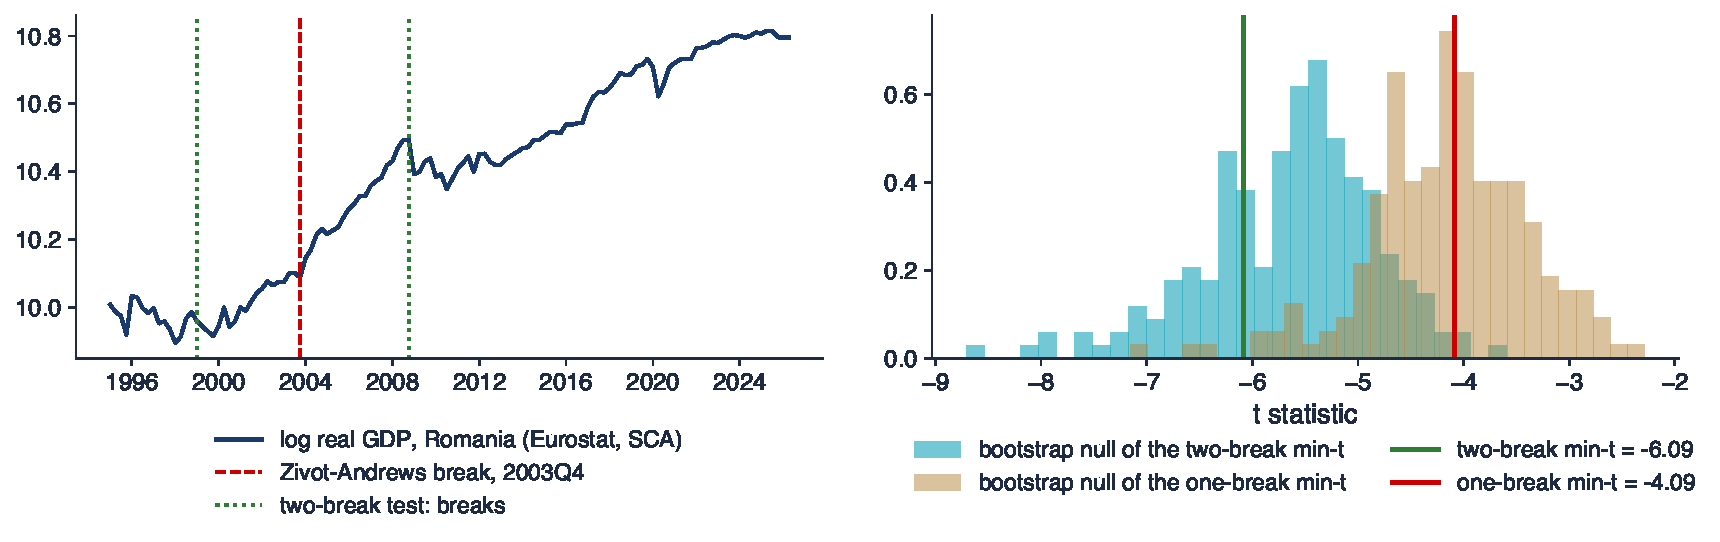
\includegraphics[width=0.97\textwidth,height=0.5\textheight,keepaspectratio]{ats_ch2_unit_root_breaks.pdf}
\end{center}
\vspace{-0.25cm}
\begin{itemize}
    \item Logaritmul PIB real (ajustat sezonier), T1 1995--T2 2026; una și două rupturi în nivel și în trend; distribuții sub $H_0$ dintr-un bootstrap sieve (AR pe $\Delta y_t$, 199 de replicări)
\end{itemize}
\quantlet{ATS\_ch2\_unit\_root\_breaks}{\qlurl{ATS_ch2_unit_root_breaks}}
\end{frame}

\begin{frame}{Interpretarea testelor de rădăcină unitară cu rupturi}
\itemsize{\small}
\begin{itemize}
    \item ADF cu trend: \ensuremath{-}2{,}79 ($p$ 0{,}201); Zivot--Andrews: \ensuremath{-}4{,}09 în T4 2003 (5\%: \ensuremath{-}5{,}07; $p$ bootstrap 0{,}523)
    \item Două rupturi (T1 1999 și T4 2008): min-$t$ = \ensuremath{-}6{,}09, valoarea bootstrap de 5\% \ensuremath{-}7{,}16, $p$ 0{,}266
    \begin{itemize}
        \item cu cît admitem mai multe rupturi, cu atît valoarea critică este mai negativă: cîștigul aparent dispare
    \end{itemize}
    \item Cu aproximativ 30 de ani de date trimestriale, rădăcina unitară nu poate fi respinsă; povestea convergenței (creștere rapidă, apoi o ruptură în 2009) rămîne o ipoteză
\end{itemize}
\end{frame}

\begin{frame}{Recapitulare: rupturile în varianță și rădăcinile unitare}
\itemsize{\small}
\begin{itemize}
    \item ICSS are nevoie de corecția $\kappa_2$ pentru cozi groase și GARCH
    \item EUR/RON: cîteva regimuri reale de varianță, nu zeci
    \item Testele de rădăcină unitară cu rupturi: admiteți rupturi sub ipoteza nulă sau testați-le în prealabil; folosiți valori critice bootstrap
\end{itemize}
\end{frame}


%=============================================================================
\section{Prognoza în prezența rupturilor}
%=============================================================================

\begin{frame}{Schimbările de nivel produc eșecul prognozelor}
\itemsize{\small}
\begin{itemize}
    \item \refCHa, \refCHb: în modelele cu corecția erorii, deplasarea mediei de echilibru este principala sursă de erori sistematice de prognoză
    \begin{itemize}
        \item după deplasare, modelul continuă să tragă prognoza spre vechea medie
    \end{itemize}
    \item Instrumente robuste
    \begin{itemize}
        \item \textbf{corecția termenului liber}: adăugăm la prognoză ultima eroare observată
        \item \textbf{diferențierea}: prognozăm $\Delta y$; se adaptează după o perioadă, cu prețul unei varianțe mai mari
        \item \textbf{ferestre mai scurte}: estimare cu fereastră mobilă sau eșantionul de după ruptură
    \end{itemize}
    \item Sinteza dovezilor: \refRos; alegerea ferestrei cu parametri variabili în timp \refIJR
\end{itemize}
\end{frame}

\begin{frame}{Alegerea ferestrei de estimare}
\itemsize{\small}
\begin{itemize}
    \item Schimbare de medie $\delta$ după $n_1$ observații înainte de ruptură, $n_2$ după; prognozăm cu ultimele $w \ge n_2$ observații \refPT
    \begin{itemize}
        \item $\mathrm{MSFE}(w) = \sigma^2\big(1 + \tfrac1w\big) + \Big(\dfrac{(w - n_2)\delta}{w}\Big)^2$: varianța scade cu $w$, pătratul deplasării crește
        \item MSFE: eroarea pătratică medie de prognoză a mediei calculate pe fereastră; $\sigma^2$: varianța zgomotului; $(w - n_2)/w$: ponderea datelor dinaintea rupturii în fereastră
        \item fereastra optimă include \emph{cîteva} date dinaintea rupturii cînd $\delta/\sigma$ este mic sau $n_2$ scurt (Seminarul 2, A8)
    \end{itemize}
    \item Reguli aplicabile: estimăm data (Bai--Perron) și folosim eșantionul de după ruptură; alegem $w$ prin validare încrucișată \refPT; mediem prognozele peste ferestre (AveW) \refPP
    \begin{itemize}
        \item data este estimată cu eroare exact cînd ruptura este mică: ferestrele de după ruptură sînt atunci prea scurte
    \end{itemize}
\end{itemize}
\end{frame}

\begin{frame}{Alegerea ferestrei: simulare și inflația din România}
\itemsize{\footnotesize}
\begin{center}
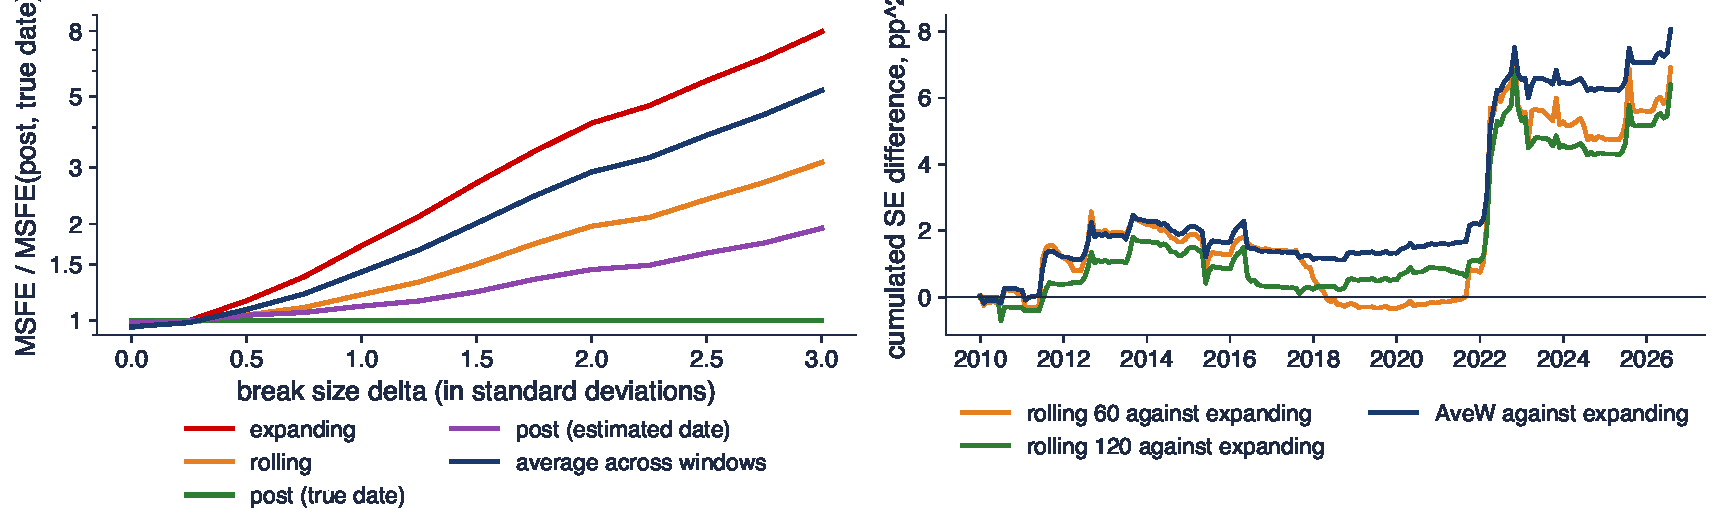
\includegraphics[width=0.97\textwidth,height=0.5\textheight,keepaspectratio]{ats_ch2_forecast_windows.pdf}
\end{center}
\vspace{-0.25cm}
\begin{itemize}
    \item Stînga: $T = 200$, ruptura cu $n_2 = 20$ de perioade înainte de final, 4\,000 de replicări, MSFE relativ la media de după ruptură cu data adevărată; dreapta: AR(2), o lună înainte, cîștigurile cumulate în eroarea pătratică față de fereastra extinsă
\end{itemize}
\quantlet{ATS\_ch2\_forecast\_windows}{\qlurl{ATS_ch2_forecast_windows}}
\end{frame}

\begin{frame}{Interpretarea alegerii ferestrei}
\itemsize{\small}
\begin{itemize}
    \item Simulare: fără ruptură cîștigă fereastra extinsă (0{,}95); cu $\delta = 1$: extinsă 1{,}71, mobilă 1{,}21, AveW 1{,}42, după ruptura estimată 1{,}11
    \begin{itemize}
        \item $\delta = 2$: 4{,}13; 1{,}97; 2{,}91; 1{,}44: estimarea datei merită cînd ruptura este mare
    \end{itemize}
    \item România, $P = 200$ de luni: RMSE extinsă 0{,}664, mobilă 60: 0{,}638, mobilă 120: 0{,}640, AveW 0{,}633 pp
    \begin{itemize}
        \item HLN față de fereastra extinsă: AveW 2{,}20 ($p$ 0{,}029), mobilă 60 1{,}19 ($p$ 0{,}234); toate cîștigurile apar în 2022, RMSE în 2021--2023 scade de la 0{,}790 la 0{,}700
    \end{itemize}
    \item Medierea peste ferestre este o asigurare ieftină: niciodată departe de cea mai bună fereastră, fără a estima vreo dată
\end{itemize}
\end{frame}

\begin{frame}{Recapitulare: prognoza în prezența rupturilor}
\itemsize{\small}
\begin{itemize}
    \item Schimbările de nivel produc eșecul prognozelor; corecția termenului liber și diferențierea fac prognozele robuste
    \item Fereastra optimă: un compromis deplasare--varianță care poate include date dinaintea rupturii
    \item AveW este robustă cînd ruptura este incertă; ferestrele de după ruptură, cînd ea este mare și bine datată
    \item Evaluați alegerea ferestrei în afara eșantionului cu DM--HLN \refDM, \refHLN\ (\atschlink{https://danpele.github.io/Advanced-Time-Series/RO/Cursuri/capitol1_evaluarea_prognozelor.pdf}{Capitolul 1})
\end{itemize}
\end{frame}


%=============================================================================
\section{Autoregresia cu prag}
%=============================================================================

\begin{frame}{Motivația modelelor neliniare}
\itemsize{\footnotesize}
\begin{columns}[T]
\begin{column}{0.36\textwidth}
\centering
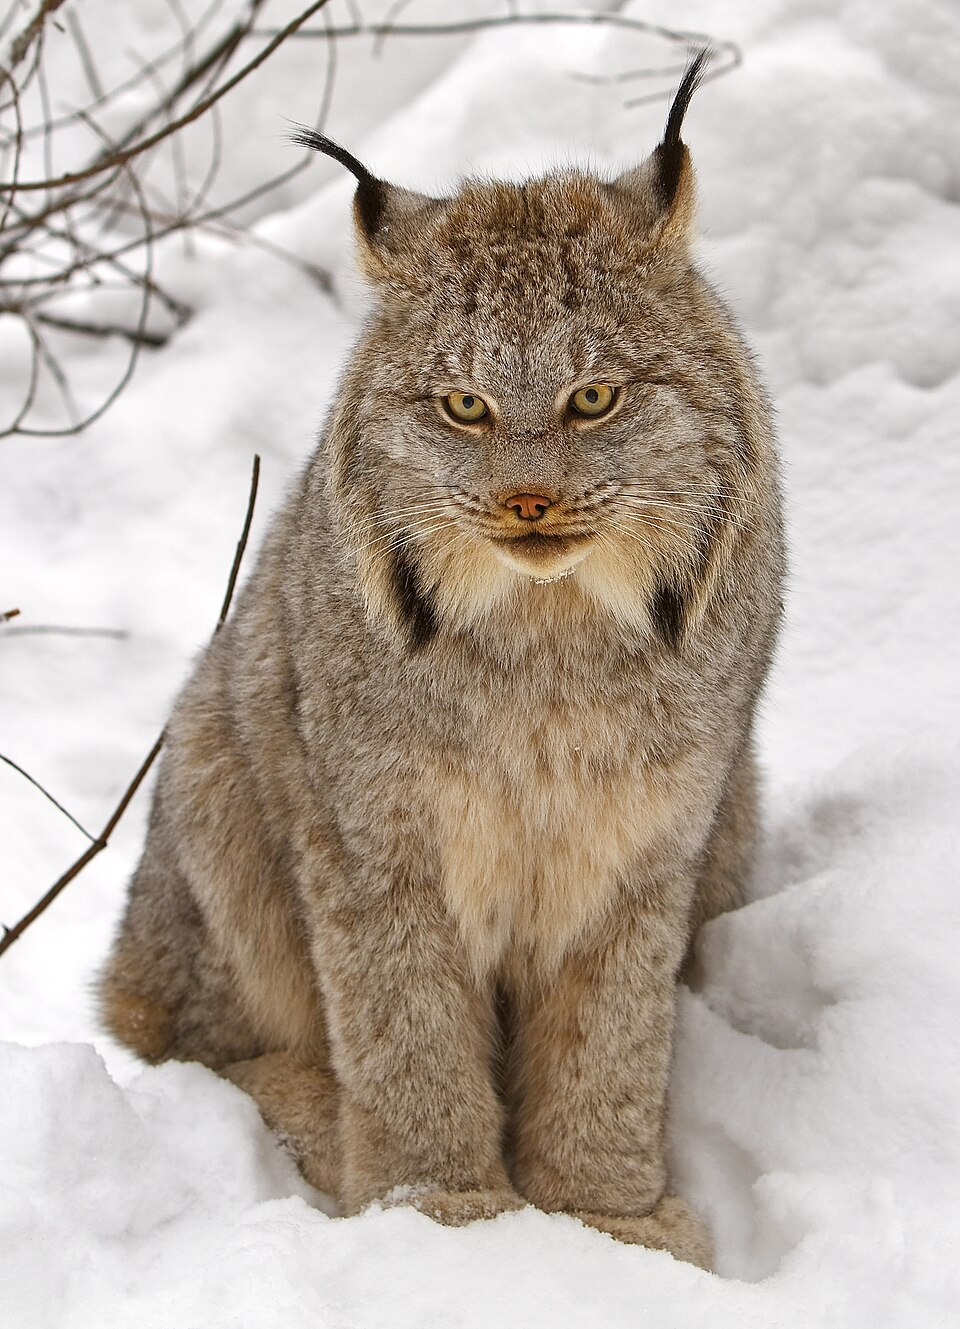
\includegraphics[height=0.36\textheight]{ch2_lynx_2010.jpg}\\[1mm]
\imgcap{Linx canadian}
\imgcredit{https://commons.wikimedia.org/wiki/File:Canada_lynx_by_Michael_Zahra_(cropped).jpg}{Foto: Michael Zahra (2010); CC BY-SA 3.0; Wikimedia Commons}
\end{column}
\begin{column}{0.62\textwidth}
\begin{itemize}
    \item Modelele liniare sînt simetrice: un șoc de $-1$ are efectul în oglindă al unui șoc de $+1$, în orice stare
    \begin{itemize}
        \item ciclurile economice: șomajul crește repede în recesiuni și scade lent în expansiuni \refNef
        \item arbitrajul: cursurile reale se mișcă liber în interiorul unei benzi a costurilor de tranzacție și revin în afara ei \refMNP
    \end{itemize}
    \item Ecologie: ciclul de 9--10 ani al linxului canadian este asimetric (creștere lentă, scădere rapidă); un AR liniar nu poate produce un ciclu stabil fără zgomot
    \item Un model neliniar poate: cicluri limită, asimetrie, persistență și răspunsuri la impuls care depind de stare
\end{itemize}
\end{column}
\end{columns}
\end{frame}

\begin{frame}{Autoregresia cu prag și autoregresia cu prag autoexcitată (1/2)}
\itemsize{\small}
\begin{itemize}
    \item \textbf{TAR} cu două regimuri: un model AR ai cărui coeficienți depind de poziția lui $q_{t-1}$ sub sau peste pragul $\gamma$
    \begin{itemize}
        \item $y_t = (\phi_{1,0} + \phi_1'\mathbf y_{t-1})\mathbf 1\{q_{t-1} \le \gamma\} + (\phi_{2,0} + \phi_2'\mathbf y_{t-1})\mathbf 1\{q_{t-1} > \gamma\} + \varepsilon_t$
        \item $\mathbf y_{t-1} = (y_{t-1}, \dots, y_{t-p})'$: ultimele $p$ valori; $\phi_{j,0}$, $\phi_j$: termenul liber și coeficienții AR ai regimului $j$
        \item $q_{t-1}$: variabila de prag, observată; $\gamma$: pragul; $\mathbf 1\{\cdot\}$ selectează regimul; varianțele pot diferi între regimuri
    \end{itemize}
    \item \textbf{SETAR} (autoexcitat): $q_{t-1} = y_{t-d}$, seria însăși, cu lagul de întîrziere (delay) $d$
    \begin{itemize}
        \item notația SETAR$(k; p_1, \dots, p_k)$: $k$ regimuri cu ordinele AR $p_1, \dots, p_k$ \refTL
    \end{itemize}
\end{itemize}
\end{frame}

\begin{frame}{Autoregresia cu prag și autoregresia cu prag autoexcitată (2/2)}
\itemsize{\small}
\begin{itemize}
    \item Dinamica: \textbf{scheletul} $y_t = F(\mathbf y_{t-1})$, modelul fără zgomot
    \begin{itemize}
        \item $F$: media condiționată, dependentă de regim; scheletul poate converge către un punct, un ciclu limită sau un atractor haotic
    \end{itemize}
    \item Staționaritatea este o proprietate a întregului model, nu a fiecărui regim
    \begin{itemize}
        \item SETAR(2; 1, 1) este ergodic dacă și numai dacă $\phi_1 < 1$, $\phi_2 < 1$ și $\phi_1\phi_2 < 1$: un regim poate fi exploziv luat separat (Seminarul 2, A5)
    \end{itemize}
    \item Sinteza modelelor cu prag în economie: \refHe
\end{itemize}
\end{frame}

\begin{frame}{Estimare și inferență (1/2)}
\itemsize{\small}
\begin{itemize}
    \item Cele mai mici pătrate concentrate: pentru fiecare $\gamma$ (și $d$) candidat aplicăm MCMMP în ambele regimuri
    \begin{itemize}
        \item $\hat\gamma = \arg\min_\gamma S_T(\gamma)$
        \item $S_T(\gamma)$: SSR total pentru un $\gamma$ dat; căutarea parcurge cele 70\% centrale ale valorilor observate ale lui $q$
        \item $\hat\gamma$ este superconsistent, $T(\hat\gamma - \gamma) = O_p(1)$, cu o limită nestandard \refChan; pantele sînt asimptotic Normale ca și cum $\gamma$ ar fi cunoscut
    \end{itemize}
    \item Testarea liniarității, $H_0$: $\phi_1 = \phi_2$: $\gamma$ nu este identificat sub $H_0$ (din nou problema Davies) \refHa
    \begin{itemize}
        \item $\sup_\gamma W_T(\gamma)$, cu $W_T(\gamma)$ statistica Wald pentru $\phi_1 = \phi_2$ la pragul $\gamma$, are o limită care depinde de date
        \item \textbf{bootstrap cu regresori ficși}: $y_t^* = \hat e_t\eta_t$, $\eta_t \sim N(0, 1)$, aceiași regresori, recalculăm $\sup W^*$; $\hat e_t$: reziduurile
    \end{itemize}
\end{itemize}
\end{frame}

\begin{frame}{Estimare și inferență (2/2)}
\itemsize{\small}
\begin{itemize}
    \item Mulțimea de încredere pentru prag \refHc: toate valorile $\gamma$ cu un raport de verosimilitate mic
    \begin{itemize}
        \item $\mathrm{LR}_T(\gamma) = T\,\dfrac{S_T(\gamma) - S_T(\hat\gamma)}{S_T(\hat\gamma)}$
        \item creșterea relativă a SSR cînd pragul este mutat de la $\hat\gamma$ la $\gamma$
    \end{itemize}
    \item Distribuția limită și valoarea critică
    \begin{itemize}
        \item $\xi = \max_s[2W(s) - |s|]$, $W$ o mișcare browniană bilaterală; $P(\xi \le x) = (1 - e^{-x/2})^2$
        \item valoarea de 95\% $-2\ln(1 - \sqrt{0{,}95}) = 7{,}35$: mulțimea de 95\% este $\{\gamma: \mathrm{LR}_T(\gamma) \le 7{,}35\}$
        \item sub heteroscedasticitate împărțim LR la $\hat\eta^2$, o corecție de tip raport de varianțe estimată din reziduuri (\atsapplink{atsapp2}{atssrc2}{Anexă})
    \end{itemize}
\end{itemize}
\end{frame}

\begin{frame}{Studiu de caz: Tong și Lim (1980), linxul canadian}
\itemsize{\small}
\begin{itemize}
    \item Lucrarea, secțiunea 9: $\log_{10}$ din numărul anual de linxi capturați, 1821--1934; SETAR(2; 7, 2) cu $d = 2$, pragul 3,116 \refTL
    \begin{itemize}
        \item $d = 2$ are o interpretare ecologică: un linx devine adult în toamna celui de-al doilea an
    \end{itemize}
    \item Replicarea noastră cu pragul din lucrare: regimul inferior $y_t = 0{,}546 + 1{,}032y_{t-1} \ensuremath{-}0{,}173y_{t-2} + \dots$ (șapte laguri), regimul superior $2{,}345 + 1{,}533y_{t-1} \ensuremath{-}1{,}276y_{t-2}$
    \begin{itemize}
        \item regimul inferior reproduce coeficienții publicați cu trei zecimale; pragul liber, după cele mai mici pătrate, este 3{,}310 (SSR 3{,}764 față de 3{,}943)
    \end{itemize}
    \item Întrebarea: generează modelul estimat, singur, ciclul linxului?
\end{itemize}
\end{frame}

\begin{frame}{Ciclul linxului și scheletul SETAR}
\itemsize{\footnotesize}
\begin{center}
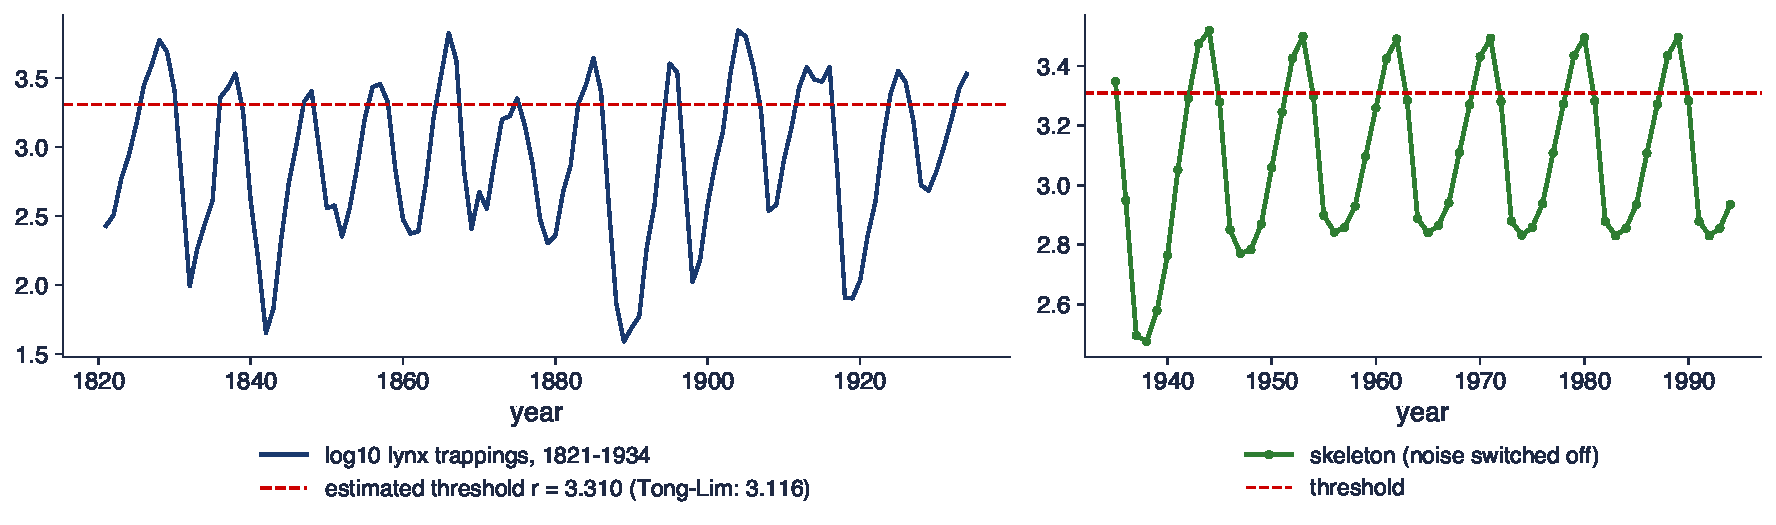
\includegraphics[width=0.97\textwidth,height=0.5\textheight,keepaspectratio]{ats_ch2_lynx.pdf}
\end{center}
\vspace{-0.25cm}
\begin{itemize}
    \item Stînga: datele și pragul estimat; dreapta: scheletul iterat 60 de ani pornind de la ultimele observații, fără zgomot
\end{itemize}
\quantlet{ATS\_ch2\_lynx}{\qlurl{ATS_ch2_lynx}}
\end{frame}

\begin{frame}{Interpretarea modelului SETAR pentru linx}
\itemsize{\small}
\begin{itemize}
    \item Scheletul se stabilizează pe un ciclu limită stabil cu perioada de 9 ani: modelul produce ciclul fără niciun zgomot
    \begin{itemize}
        \item un AR(11) liniar are nevoie de zgomot pentru a întreține oscilația; scheletul lui converge la medie
    \end{itemize}
    \item Creșterea este lentă (regimul inferior, șapte laguri), scăderea rapidă (regimul superior, un AR(2) exploziv luat separat): asimetria din date
    \item Varianța reziduală 0{,}0352 față de 0{,}0364 pentru AR(11): un cîștig mic în eșantion, un cîștig mare în descrierea dinamicii
\end{itemize}
\end{frame}

\begin{frame}{Studiu de caz: Hansen (1997), șomajul din SUA}
\itemsize{\small}
\begin{itemize}
    \item Lucrarea, secțiunea 5: rata șomajului bărbaților de 20 de ani și peste (șomeri / forța de muncă), lunar 1959.1--1996.7; $\Delta y_t$ pe o constantă și 12 laguri \refHb
    \begin{itemize}
        \item $y_t$: rata șomajului, în \%; variabila de prag $q_{t-1} = y_{t-1} - y_{t-d}$, $d = 2, \dots, 12$: variația din ultimele $d - 1$ luni; trunchiere 15\%
        \item test sup-Wald robust, p-value-uri bootstrap (1000 de replicări); estimarea LS $\hat d = 12$, $\hat\gamma = 0{,}302$, intervalul de 95\% [0,213; 0,340], 314 și 124 de observații
    \end{itemize}
    \item Replicarea noastră: aceeași construcție din seriile BLS de pe FRED (ajustarea sezonieră de azi), același model, $d = 12$
    \item Întrebarea: există un „regim de recesiune” cu altă dinamică și cît de precis este estimat pragul lui?
\end{itemize}
\end{frame}

\begin{frame}{Un model cu prag pentru șomajul din SUA}
\itemsize{\footnotesize}
\begin{center}
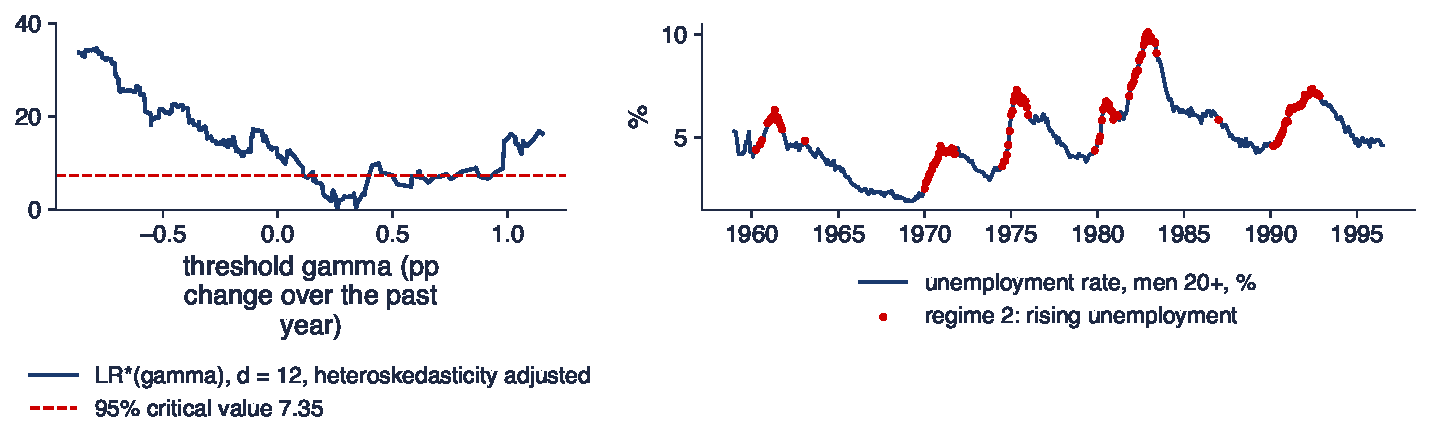
\includegraphics[width=0.97\textwidth,height=0.5\textheight,keepaspectratio]{ats_ch2_unemp_tar.pdf}
\end{center}
\vspace{-0.25cm}
\begin{itemize}
    \item Stînga: $\mathrm{LR}^*(\gamma)$ ajustat pentru heteroscedasticitate, $d = 12$; mulțimea de 95\% este acolo unde curba se află sub 7,35. Dreapta: lunile din regimul cu șomaj în creștere ($q_{t-1} > \hat\gamma$)
\end{itemize}
\quantlet{ATS\_ch2\_unemp\_tar}{\qlurl{ATS_ch2_unemp_tar}}
\end{frame}

\begin{frame}{Interpretarea modelului TAR pentru șomaj}
\itemsize{\footnotesize}
\begin{itemize}
    \item $\hat\gamma = 0{,}261$ pp (lucrarea: 0,302), regimuri de 314 și 124 de luni, aceeași împărțire ca la \refHb; mulțimea de 95\% [0{,}131; 0{,}917]
    \begin{itemize}
        \item sup-Wald 47{,}2, p-value bootstrap 0{,}015; liniaritatea este respinsă la 5\% pentru 10 din cele 11 laguri $d$
    \end{itemize}
    \item Regimul de creștere: termen liber 0{,}065, AR(1) 0{,}18, AR(2) 0{,}28; celelalte luni: \ensuremath{-}0{,}019; \ensuremath{-}0{,}15; 0{,}06
    \begin{itemize}
        \item creșterile se autoalimentează; în expansiune șomajul este aproape un mers aleator cu o ușoară tendință descendentă
    \end{itemize}
    \item Cu datele de azi, SSR este minim la $d = 3$ ($\hat\gamma = \ensuremath{-}0{,}24$): lagul $d$ este fragil, efectul de prag nu; 1959--2019: $\hat\gamma = 0{,}261$, $p$ $<$\,0{,}001
\end{itemize}
\end{frame}

\begin{frame}{Recapitulare: autoregresia cu prag}
\itemsize{\small}
\begin{itemize}
    \item Un AR liniar pe porțiuni care comută după o variabilă observată; poate genera cicluri limită
    \item $\hat\gamma$ superconsistent; pantele ca și cum $\gamma$ ar fi cunoscut
    \item Testele de liniaritate au nevoie de bootstrap; intervalele pentru prag inversează LR cu valoarea 7,35
    \item Linxul și șomajul: ambele rezultate de referință se replică
\end{itemize}
\end{frame}


%=============================================================================
\section{Autoregresia cu tranziție netedă}
%=============================================================================

\begin{frame}{Modelele STAR (1/2)}
\itemsize{\small}
\begin{itemize}
    \item O medie ponderată a două regimuri AR, cu o pondere $G$ care variază continuu între 0 și 1 \refTer
    \begin{itemize}
        \item $y_t = \phi_1'\mathbf x_t[1 - G(s_t; \gamma, c)] + \phi_2'\mathbf x_t G(s_t; \gamma, c) + \varepsilon_t$, $\quad \mathbf x_t = (1, y_{t-1}, \dots, y_{t-p})'$
        \item $s_t$: variabila de tranziție (de exemplu un lag al lui $y_t$); $c$: locul tranziției; $\gamma > 0$: viteza ei
        \item $G = 0$: regimul 1, cu coeficienții $\phi_1$; $G = 1$: regimul 2, cu $\phi_2$; între ele, o combinație
    \end{itemize}
    \item Un continuu de regimuri
    \begin{itemize}
        \item agregarea mai multor agenți cu praguri diferite sau agregarea temporală produc o comutare netedă
    \end{itemize}
\end{itemize}
\end{frame}

\begin{frame}{Modelele STAR (2/2)}
\itemsize{\small}
\begin{itemize}
    \item \textbf{LSTAR} (logistic): valori mici față de valori mari ale lui $s_t$
    \begin{itemize}
        \item $G = [1 + \exp\{-\gamma(s_t - c)/\hat\sigma_s\}]^{-1}$
        \item $\gamma \to \infty$ dă TAR, $\gamma \to 0$ dă AR liniar; $\hat\sigma_s$: abaterea standard a lui $s_t$, care face ca $\gamma$ să nu depindă de scală și să fie mai ușor de estimat
    \end{itemize}
    \item \textbf{ESTAR} (exponențial): \emph{abateri} mici față de abateri mari de la $c$, simetric
    \begin{itemize}
        \item $G = 1 - \exp\{-\gamma(s_t - c)^2\}$
    \end{itemize}
    \item Sinteză cu ciclul de modelare (specificare, estimare, evaluare): \refVDTF
\end{itemize}
\end{frame}

\begin{frame}{Testarea liniarității față de STAR}
\itemsize{\small}
\begin{itemize}
    \item Sub $H_0$: $\gamma = 0$, parametrii $c$ și $\phi_2$ nu sînt identificați: înlocuim $G$ printr-o dezvoltare Taylor de ordinul trei în jurul lui $\gamma = 0$ \refLST
    \begin{itemize}
        \item regresia auxiliară $\hat\varepsilon_t = \beta_0'\mathbf x_t + \beta_1'\tilde{\mathbf x}_t s_t + \beta_2'\tilde{\mathbf x}_t s_t^2 + \beta_3'\tilde{\mathbf x}_t s_t^3 + v_t$
        \item $\hat\varepsilon_t$: reziduurile AR-ului liniar; $\tilde{\mathbf x}_t$: $\mathbf x_t$ fără constantă; $\beta_k$: coeficienții interacțiunilor cu $s_t^k$; $v_t$: eroarea
        \item LM3: $\beta_1 = \beta_2 = \beta_3 = 0$, un test $F$ cu $3p$ restricții; repetăm pentru fiecare $s_t$ candidat și alegem cel mai mic p-value (derivarea în \atsapplink{atsapp3}{atssrc3}{Anexă})
    \end{itemize}
    \item \textbf{Alegerea familiei} \refTer: testăm $H_{04}$: $\beta_3 = 0$, apoi $H_{03}$: $\beta_2 = 0 \mid \beta_3 = 0$, apoi $H_{02}$: $\beta_1 = 0 \mid \beta_2 = \beta_3 = 0$
    \begin{itemize}
        \item cea mai puternică respingere pentru $H_{03}$: ESTAR; pentru $H_{04}$ sau $H_{02}$: LSTAR (un ESTAR nu are termen cubic în dezvoltare)
    \end{itemize}
    \item Estimarea prin cele mai mici pătrate neliniare, cu parametrii liniari concentrați; evaluarea prin teste LM pentru neliniaritate reziduală și constanța parametrilor \refET
\end{itemize}
\end{frame}

\begin{frame}{Studiu de caz: van Dijk, Teräsvirta și Franses (2002)}
\itemsize{\small}
\begin{itemize}
    \item Lucrarea, secțiunea 7: rata neajustată a șomajului bărbaților de 20 de ani și peste din SUA, iunie 1968--decembrie 1999; estimare pînă în 1989, prognoze pentru 1990--1999 \refVDTF
    \begin{itemize}
        \item $\Delta y_t$ pe o constantă, 11 variabile dummy lunare, $y_{t-1}$ și 15 laguri ale lui $\Delta y_t$; variabila de tranziție $s_t = \Delta_{12}y_{t-d}$ (variația pe 12 luni, cu lagul $d$), $d = 1, \dots, 6$
        \item LSTAR-ul lor cu $d = 1$: $\hat\gamma = 23{,}15$, $\hat c = 0{,}27$, abaterea standard reziduală 0,92 din cea a AR
    \end{itemize}
    \item Replicarea noastră: aceeași serie (BLS prin FRED), același eșantion, aceiași regresori și aceeași tranziție; lagurile nerestricționate, fără eliminarea termenilor nesemnificativi din lucrare
    \item Întrebarea: bate un LSTAR modelul liniar în afara eșantionului?
\end{itemize}
\end{frame}

\begin{frame}{Un LSTAR pentru șomajul din SUA}
\itemsize{\footnotesize}
\begin{center}
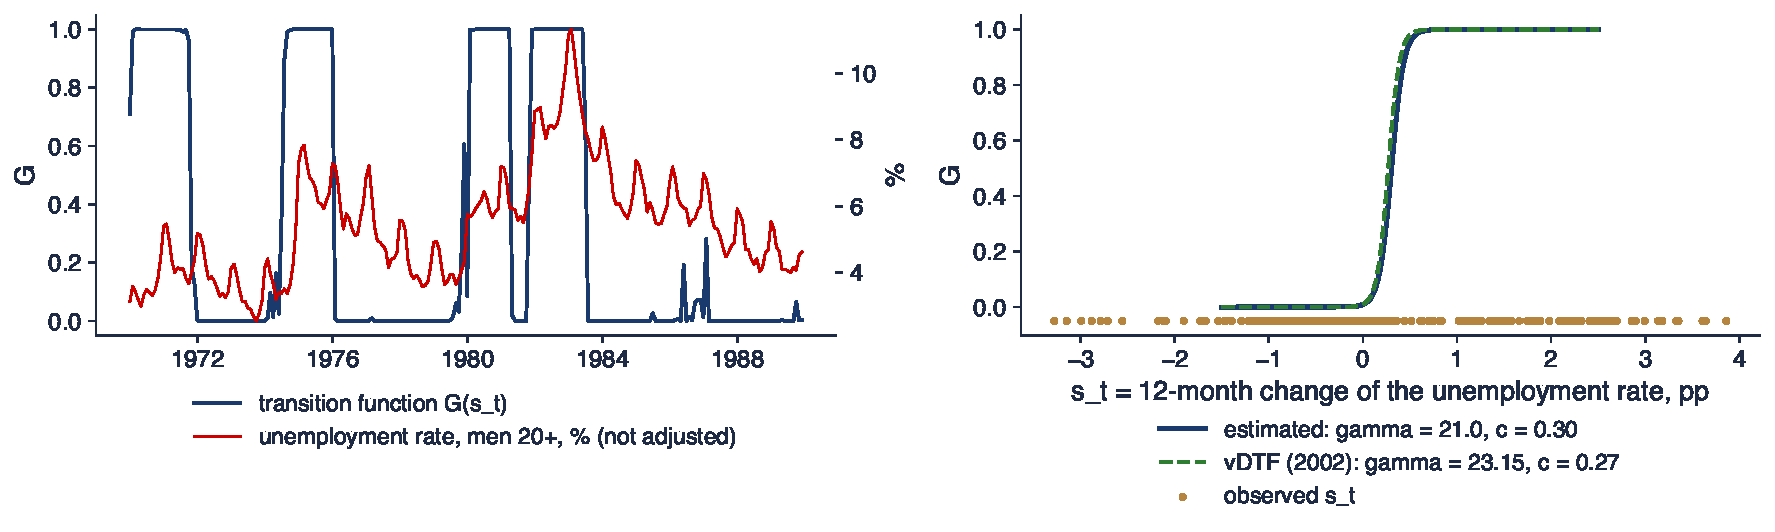
\includegraphics[width=0.97\textwidth,height=0.5\textheight,keepaspectratio]{ats_ch2_unemp_lstar.pdf}
\end{center}
\vspace{-0.25cm}
\begin{itemize}
    \item Stînga: funcția de tranziție estimată în timp, împreună cu rata șomajului; dreapta: $G$ ca funcție de $s_t = \Delta_{12}y_{t-1}$, a noastră și cea publicată
\end{itemize}
\quantlet{ATS\_ch2\_unemp\_lstar}{\qlurl{ATS_ch2_unemp_lstar}}
\end{frame}

\begin{frame}{Interpretarea modelului LSTAR}
\itemsize{\footnotesize}
\begin{itemize}
    \item P-value-urile LM3: $d = 1$: 0{,}124, $d = 2$: 0{,}052, $d = 3$: 0{,}275; pentru $d = 2$: $H_{04}$ 0{,}008, $H_{03}$ 0{,}548, $H_{02}$ 0{,}461: LSTAR
    \begin{itemize}
        \item în acord cu \refVDTF: dovezi slabe, cele mai puternice pentru $d = 2$, care indică familia logistică
    \end{itemize}
    \item $\hat\gamma = 21{,}0$, $\hat c = 0{,}30$, raportul abaterilor standard reziduale 0{,}90; regimul se schimbă cînd șomajul a crescut cu aproximativ 0,3 pp într-un an ($G > 0{,}5$ în 32\% din luni)
    \begin{itemize}
        \item AIC preferă LSTAR (\ensuremath{-}3{,}034 față de \ensuremath{-}2{,}979); BIC, modelul liniar (\ensuremath{-}2{,}573 față de \ensuremath{-}2{,}366): 18 parametri în plus, fără eliminare
    \end{itemize}
    \item 1990--1999, un pas: RMSE 0{,}218 (LSTAR) față de 0{,}228 (AR), HLN 1{,}14, $p$ 0{,}255: mai bun, dar nu semnificativ
\end{itemize}
\end{frame}

\begin{frame}{Cursurile reale și paritatea puterii de cumpărare}
\itemsize{\footnotesize}
\begin{columns}[T]
\begin{column}{0.34\textwidth}
\centering
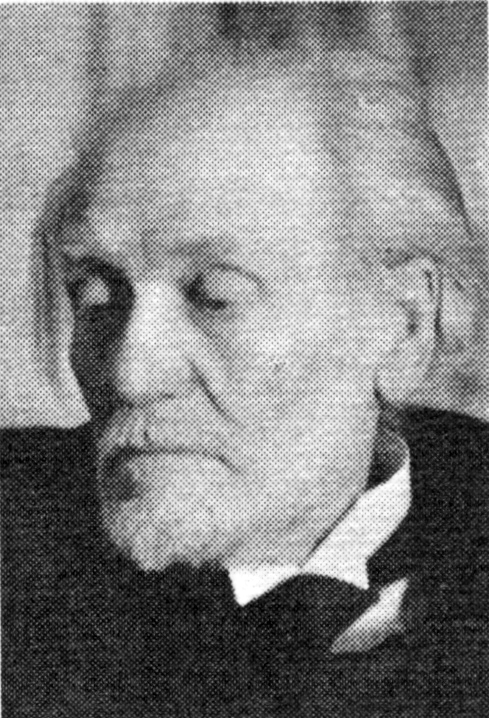
\includegraphics[height=0.24\textheight]{ch2_cassel.jpg}\\[1mm]
\imgcap{Gustav Cassel (1866--1945)}
\imgcredit{https://commons.wikimedia.org/wiki/File:Gustav_Cassel.jpg}{Portret: autor necunoscut; domeniu public; Wikimedia Commons}\\[1mm]\centering

\includegraphics[height=0.15\textheight]{ch2_bretton_woods_1944.jpg}\\[1mm]
\imgcap{Bretton Woods, iulie 1944}
\imgcredit{https://commons.wikimedia.org/wiki/File:Morgenthau_Bretton_Woods_opening_1944.jpg}{Foto: US National Archives (1944); domeniu public; Wikimedia Commons}
\end{column}
\begin{column}{0.64\textwidth}
\begin{itemize}
    \item Paritatea puterii de cumpărare, PPC (Cassel, 1918): cursul real $q_t = s_t - p_t + p_t^*$ ar trebui să fie staționar
    \begin{itemize}
        \item $s_t$: logaritmul cursului nominal (moneda națională pentru o unitate de monedă străină); $p_t$, $p_t^*$: logaritmii nivelurilor prețurilor interne și externe
        \item după sfîrșitul sistemului Bretton Woods (1973), testele de rădăcină unitară resping rar
        \item primul paradox PPC: nicio revenire la medie; al doilea: timpi de înjumătățire de 3--5 ani, prea lenți pentru șocuri nominale
    \end{itemize}
    \item Costurile de tranzacție creează o bandă de inacțiune: aproape de paritate $q_t$ este aproape un mers aleator, departe de ea arbitrajul îl trage înapoi \refMNP
    \begin{itemize}
        \item \refTPS: ESTAR $q_t - \mu = (q_{t-1} - \mu)\exp\{-\theta^2(q_{t-1} - \mu)^2\} + \varepsilon_t$
        \item $\mu$: echilibrul; aproape de el coeficientul AR $\exp\{\cdot\}$ este aproape de 1 (mers aleator), departe de el aproape de 0 (revenire rapidă); $\theta^2$: viteza
    \end{itemize}
\end{itemize}
\end{column}
\end{columns}
\end{frame}

\begin{frame}{Studiu de caz: Taylor, Peel și Sarno (2001)}
\itemsize{\small}
\begin{itemize}
    \item Lucrarea: cursurile reale lunare ale lirei sterline, mărcii, francului și yenului față de dolar, 1973M01--1996M12, date FMI IFS, $q(1973M01) = 0$; ESTAR cu $p = d = 1$ și $\beta_1 = -\beta_1^* = 1$ (ec.\ 8) \refTPS
    \begin{itemize}
        \item dolar--liră: $\hat\theta^2 = 0{,}452$, $\hat\mu = -0{,}149$, $s = 0{,}033$ (abaterea standard reziduală); p-value-ul Monte Carlo al lui $\hat\theta$ sub un mers aleator: 0,002
        \item timpi de înjumătățire din răspunsuri la impuls generalizate, condiționate de istoria medie: sub un an pentru un șoc de 40\%, puțin sub trei ani pentru 1\%
    \end{itemize}
    \item Replicarea noastră pentru dolar--liră: DEXUSUK la sfîrșit de lună, IPC SUA (CPIAUCNS), IPC britanic (OECD pînă în 1987, apoi ONS); același model, aceeași procedură pentru timpii de înjumătățire; extensie pînă în august 2026
    \item Întrebarea: revine cursul real neliniar la medie și cît de repede?
\end{itemize}
\end{frame}

\begin{frame}{Revenirea neliniară la medie a cursului real dolar--liră}
\itemsize{\footnotesize}
\begin{center}
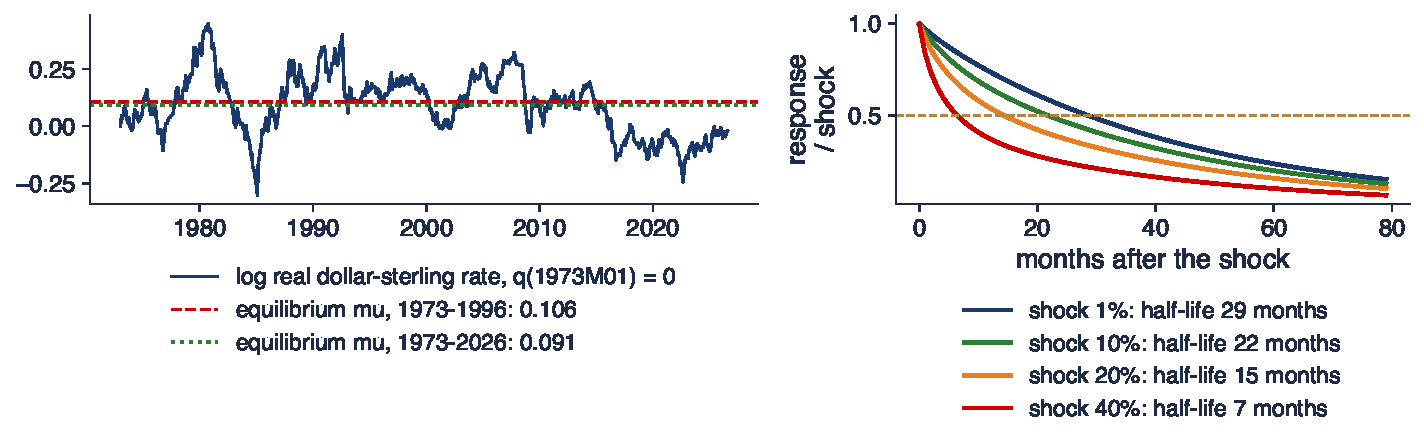
\includegraphics[width=0.97\textwidth,height=0.5\textheight,keepaspectratio]{ats_ch2_ppp_estar.pdf}
\end{center}
\vspace{-0.25cm}
\begin{itemize}
    \item Stînga: $q_t$ și echilibrele estimate; dreapta: răspunsurile la impuls generalizate ale ESTAR 1973--1996, șocuri de 1--40\%, mediate peste istoriile observate
\end{itemize}
\quantlet{ATS\_ch2\_ppp\_estar}{\qlurl{ATS_ch2_ppp_estar}}
\end{frame}

\begin{frame}{Interpretarea modelului ESTAR}
\itemsize{\footnotesize}
\begin{itemize}
    \item 1973--1996: $\hat\theta^2 = 0{,}527$ (eroarea standard 0{,}219), $\hat\mu = 0{,}106$, $s = 0{,}033$; p-value-ul Monte Carlo al raportului $t$ 0{,}165 (lucrarea: 0,002)
    \begin{itemize}
        \item $\theta^2$ și $s$ sînt apropiate de lucrare; $\mu$ diferă pentru că IPC britanic din lucrare (IFS) nu este seria publicată astăzi
    \end{itemize}
    \item Timpi de înjumătățire: șoc de 1\% 29 de luni, 10\% 22, 40\% 7; AR(1) liniar: 21 de luni; din echilibru: 42 de luni pentru 1\%
    \begin{itemize}
        \item abaterile mari se sting repede: al doilea paradox PPC este o trăsătură a șocurilor mici
    \end{itemize}
    \item Dickey--Fuller: \ensuremath{-}2{,}20 ($p$ 0{,}205); puterea lui față de ESTAR-ul nostru este 19\%
    \item KSS \refKSS: \ensuremath{-}2{,}47 ($p$ 0{,}144) pînă în 1996, \ensuremath{-}3{,}47 ($p$ 0{,}014) pînă în 2026
    \begin{itemize}
        \item statistica $t$ a lui $\delta$ în $\Delta q_t = \delta q_{t-1}^3 + e_t$ ($q_t$ cu media scăzută): test de rădăcină unitară față de un ESTAR staționar; respingem în coada stîngă
    \end{itemize}
\end{itemize}
\end{frame}

\begin{frame}{Recapitulare: tranziția netedă}
\itemsize{\small}
\begin{itemize}
    \item LSTAR: asimetrie între stările joase și înalte; ESTAR: abateri mici și mari
    \item Testele LM dintr-o dezvoltare Taylor evită problema identificării; secvența $H_{04}$, $H_{03}$, $H_{02}$ alege familia
    \item Șomajul: LSTAR-ul publicat se replică; cîștigul lui de prognoză este mic
    \item PPC: timpii de înjumătățire depind de mărimea șocului; dovezile de neliniaritate depind de eșantion
\end{itemize}
\end{frame}


%=============================================================================
\section{Teste de neliniaritate}
%=============================================================================

\begin{frame}{Teste generale și teste specifice}
\itemsize{\small}
\begin{itemize}
    \item \textbf{BDS} \refBDSL: integrala de corelație $C_{m}(\varepsilon)$ a istoriilor de lungime $m$; sub i.i.d.\ $C_m = C_1^m$; se aplică reziduurilor unui model liniar
    \begin{itemize}
        \item $C_m(\varepsilon)$: proporția perechilor de istorii de lungime $m$, $(y_t, \dots, y_{t+m-1})$, aflate la distanță mai mică decît $\varepsilon$ în fiecare coordonată
        \item putere împotriva oricărei dependențe rămase în reziduuri, inclusiv ARCH: o respingere nu spune ce neliniaritate este
    \end{itemize}
    \item \textbf{Keenan} (valorile ajustate la pătrat) și testul din \refTsa\ (toate produsele $y_{t-i}y_{t-j}$, ortogonalizate): teste $F$ pentru termeni Volterra de ordinul doi
    \begin{itemize}
        \item testul lui Tsay cu autoregresie ordonată vizează alternativa TAR \refTsb
    \end{itemize}
    \item \textbf{LM3} (STAR) și \textbf{sup-Wald} (TAR): alternative specifice, mai multă putere cînd sînt corecte
    \begin{itemize}
        \item atenție: rupturile structurale, valorile extreme și heteroscedasticitatea resping și ele liniaritatea \refCar
    \end{itemize}
\end{itemize}
\end{frame}

\begin{frame}{Cinci serii, cinci teste}
\itemsize{\footnotesize}
\begin{center}
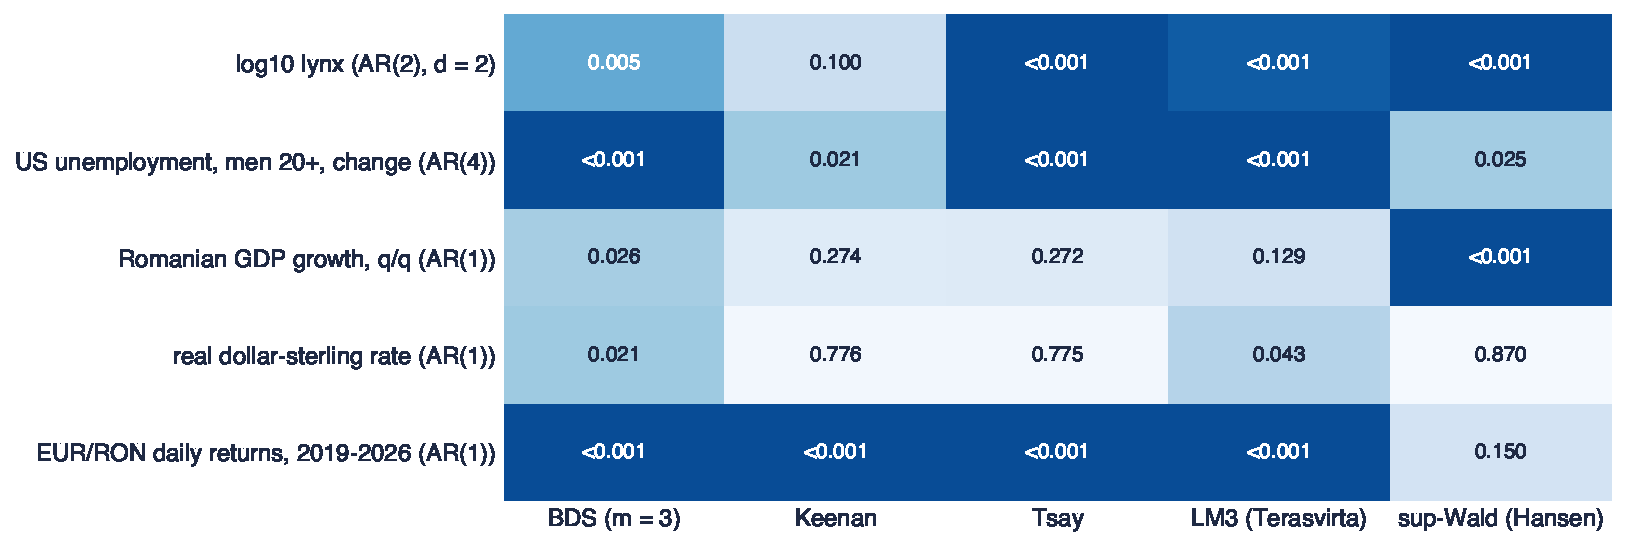
\includegraphics[width=0.97\textwidth,height=0.5\textheight,keepaspectratio]{ats_ch2_nonlinearity_tests.pdf}
\end{center}
\vspace{-0.25cm}
\begin{itemize}
    \item P-value-uri; mai închis: respingere mai puternică a liniarității. BDS pe reziduurile AR ($m = 3$, $\varepsilon = \hat\sigma$); LM3 și sup-Wald cu $s = q = y_{t-d}$; sup-Wald cu 200 de replicări bootstrap
\end{itemize}
\quantlet{ATS\_ch2\_nonlinearity\_tests}{\qlurl{ATS_ch2_nonlinearity_tests}}
\end{frame}

\begin{frame}{Interpretarea bateriei de teste}
\itemsize{\small}
\begin{itemize}
    \item Linxul și șomajul: toate testele specifice resping; neliniaritatea este reală și de tipul cu prag
    \item Randamentele EUR/RON: BDS, Keenan, Tsay și LM3 resping toate cu $p$ $<$\,0{,}001, dar sup-Wald pentru TAR nu ($p$ 0{,}150)
    \begin{itemize}
        \item volatility clustering și valori extreme, nu o medie condiționată neliniară: testul robust la heteroscedasticitate este cel corect
    \end{itemize}
    \item Creșterea PIB din România: doar BDS și sup-Wald resping ($p$ $<$\,0{,}001): trimestrele din 2009 și 2020 acționează ca un „regim”; un model cu ruptură sau cu valori extreme poate explica aceleași date
\end{itemize}
\end{frame}

\begin{frame}{Cointegrarea cu prag}
\itemsize{\small}
\begin{itemize}
    \item \refBF: termenul de corecție a erorii $z_t = y_t - \beta x_t$ se ajustează doar în afara unei benzi: $\Delta z_t = \rho\,z_{t-1}\mathbf 1\{|z_{t-1}| > \gamma\} + \varepsilon_t$
    \begin{itemize}
        \item $y_t, x_t$: două prețuri cointegrate; $\beta$: coeficientul de cointegrare; $\rho < 0$: viteza de ajustare în afara benzii $[-\gamma, \gamma]$
        \item același argument al costurilor de tranzacție ca la ESTAR, pentru o pereche de prețuri: prețul unei mărfuri pe două piețe, transmiterea dobînzilor, legea prețului unic
    \end{itemize}
    \item Ajustare asimetrică (TAR cu momentum) \refES; testul VECM liniar față de VECM cu prag, cu bootstrap \refHS
    \begin{itemize}
        \item \atschlink{https://danpele.github.io/Advanced-Time-Series/RO/Cursuri/capitol4_cointegrare_vecm_ardl_panel.pdf}{Capitolul 4} introduce VECM liniar și ARDL; variantele cu prag sînt o extensie naturală de proiect
    \end{itemize}
    \item Exemplu românesc: transmiterea de la dobînda de politică monetară a BNR la ROBOR și la dobînzile la credite, cu o bandă în care băncile nu se ajustează
\end{itemize}
\end{frame}


%=============================================================================
\section{Prognoza cu modele neliniare}
%=============================================================================

\begin{frame}{Prognozele pe mai mulți pași nu sînt scheletul}
\itemsize{\small}
\begin{itemize}
    \item Pentru $h = 1$: $\E(y_{t+1}\mid\mathcal F_t) = F(\mathbf y_t)$; pentru $h \ge 2$: $\E[F(F(\mathbf y_t) + \varepsilon_{t+1}, \dots)] \ne F(F(\mathbf y_t))$ (Jensen)
    \begin{itemize}
        \item $F$: funcția medie condiționată a modelului; Jensen: media unei funcții neliniare nu este funcția mediei
        \item iterarea scheletului (prognoza „naivă”) este deplasată; simulăm traiectorii cu reziduuri bootstrap și le mediem \refCFS
        \item densitatea predictivă poate fi asimetrică sau bimodală: raportați densități, evaluate cu CRPS sau scorul logaritmic (\atschlink{https://danpele.github.io/Advanced-Time-Series/RO/Cursuri/capitol1_evaluarea_prognozelor.pdf}{Capitolul 1})
    \end{itemize}
    \item Dovezi: modelele neliniare bat rar modelele liniare în medie; cîștigurile se concentrează în anumite regimuri (recesiuni) \refMZTT, \refTDM
    \begin{itemize}
        \item evaluați condiționat: teste GW cu regimul ca instrument (\atschlink{https://danpele.github.io/Advanced-Time-Series/RO/Cursuri/capitol1_evaluarea_prognozelor.pdf}{Capitolul 1}); dinamica asimetrică a șomajului din SUA \refKPo
    \end{itemize}
\end{itemize}
\end{frame}

\begin{frame}{Prognoze TAR și AR pentru șomajul din SUA}
\itemsize{\footnotesize}
\begin{center}
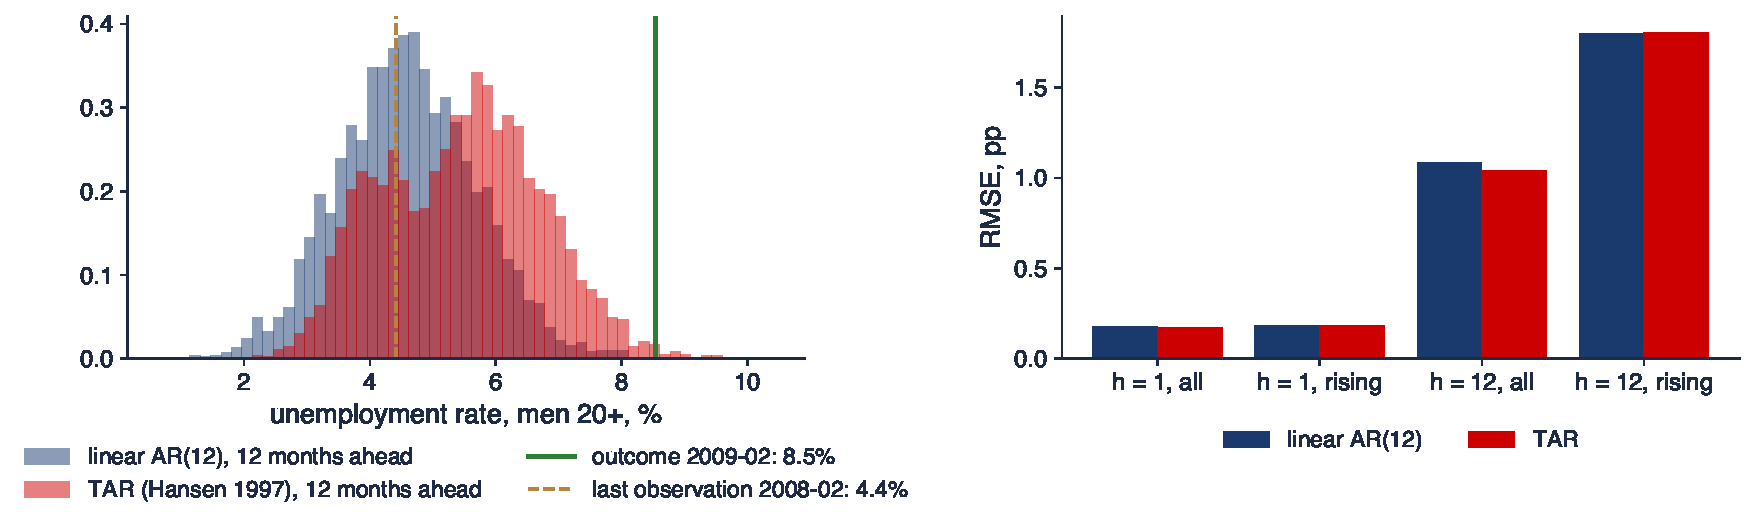
\includegraphics[width=0.97\textwidth,height=0.5\textheight,keepaspectratio]{ats_ch2_nonlinear_forecasts.pdf}
\end{center}
\vspace{-0.25cm}
\begin{itemize}
    \item TAR-ul lui Hansen ($d = 12$) și un AR(12) liniar în diferențe, parametri ficși din 1959--1996; prognoze ale nivelului prin 500 de traiectorii simulate, origini 1996--2019. Stînga: densitățile la 12 luni din februarie 2008
\end{itemize}
\quantlet{ATS\_ch2\_nonlinear\_forecasts}{\qlurl{ATS_ch2_nonlinear_forecasts}}
\end{frame}

\begin{frame}{Interpretarea prognozelor neliniare}
\itemsize{\small}
\begin{itemize}
    \item Din februarie 2008 (înainte de creșterea din 2008--2009): media TAR 5{,}5\%, intervalul de 90\% [3{,}5; 7{,}5]; media AR 4{,}6\%, [2{,}9; 6{,}4]; realizarea 8{,}5\%
    \begin{itemize}
        \item densitatea TAR este asimetrică spre valori mari odată ce șomajul începe să crească; niciun model nu a anticipat mărimea recesiunii
    \end{itemize}
    \item $P = 270$ de luni: RMSE la o lună 0{,}173 (TAR) față de 0{,}177 (AR), HLN 1{,}12 ($p$ 0{,}265); la 12 luni 1{,}039 față de 1{,}087 ($p$ 0{,}599)
    \begin{itemize}
        \item în cele 62 de luni din regimul de creștere cele două sînt egale la 12 luni (1{,}802 și 1{,}801): niciun cîștig specific regimului în afara eșantionului
    \end{itemize}
    \item O neliniaritate bună în eșantion nu este un cîștig de prognoză: preînregistrați comparația
\end{itemize}
\end{frame}

\begin{frame}{Recapitulare: testele de neliniaritate și prognozele}
\itemsize{\small}
\begin{itemize}
    \item Testele generale (BDS, Keenan, Tsay) detectează, cele specifice (LM3, sup-Wald) descriu
    \item Heteroscedasticitatea, valorile extreme și rupturile resping și ele liniaritatea
    \item Prognozele neliniare pe mai mulți pași cer simulare; raportați densități
    \item În afara eșantionului, modelele neliniare cîștigă puțin în medie; testați acolo unde ar trebui să cîștige
\end{itemize}
\end{frame}


%=============================================================================
\section{AI în descoperirea științifică}
%=============================================================================

\begin{frame}{O întrebare deschisă}
\itemsize{\small}
\begin{itemize}
    \item Neliniaritate sau rupturi? Cîteva schimbări ale mediei pot arăta ca o revenire neliniară la medie, iar un model cu prag poate arăta ca un șir de rupturi \refCar, \refDI
    \begin{itemize}
        \item formal: rezistă respingerea KSS (ESTAR) pentru cursul real dolar--liră la regimurile de medie Bai--Perron estimate pe aceleași date?
        \item infirmată dacă respingerea dispare odată ce distribuția sub ipoteza nulă ține cont de rupturile estimate
    \end{itemize}
    \item De ce contează: timpii de înjumătățire, PPC și credibilitatea modelelor de curs depind de povestea adevărată
    \begin{itemize}
        \item literatura de pornire: \refTPS, \refKSS, \refMNP, \refCar, \refBPb
    \end{itemize}
\end{itemize}
\end{frame}

\begin{frame}{Bucla de cercetare cu un asistent AI}
\itemsize{\footnotesize}
\begin{itemize}
    \item Un asistent AI (un LLM precum Claude, ChatGPT, Gemini sau Copilot) accelerează fiecare etapă; Semantic Scholar și Elicit ajută la literatură
    \begin{itemize}
        \item \textbf{literatura}: \aiprompt{Listează articole recenzate care testează modele ESTAR pentru cursul real permițînd rupturi în medie; dă DOI-urile.} Apoi verificați fiecare DOI pe Crossref
        \item \textbf{ipoteza}: \aiprompt{Propune un proces generator de date cu rupturi în medie și fără neliniaritate care face testul KSS să respingă.}
        \item \textbf{cod și replicare}: reproduceți întîi o cifră din acest curs (statistica KSS pînă în 2026), apoi noua procedură
        \item \textbf{robustețe și critică}: \aiprompt{Joacă rolul unui recenzent: enumeră toate felurile în care estimarea rupturilor pe aceleași date deplasează testul.}
    \end{itemize}
    \item Raportul: ce s-a cerut, ce s-a păstrat, ce s-a respins (AI\_USE.md, AI\_ERRORS.md)
\end{itemize}
\end{frame}

\begin{frame}{Verificări necesare}
\itemsize{\small}
\begin{itemize}
    \item Fiecare referință există și spune ce se afirmă (DOI-ul funcționează, titlul coincide, rezultatul se află în lucrare)
    \item Distribuția sub ipoteza nulă reproduce întreaga procedură: rupturile se estimează pe fiecare serie simulată, nu se fixează la datele observate
    \item Numărul rupturilor, trunchierea și criteriul (BIC) sînt fixate înainte de a vedea rezultatul testului
    \item Datele sînt seriile publicate (versiunea, deflatorul, sfîrșitul lunii); diferențele față de lucrare sînt raportate
    \item „Nesemnificativ în interiorul regimurilor” nu înseamnă „liniar”: raportați puterea procedurii
\end{itemize}
\end{frame}

\begin{frame}{Mini-studiu de caz: dovezi ESTAR sau schimbări de medie?}
\itemsize{\footnotesize}
\begin{center}
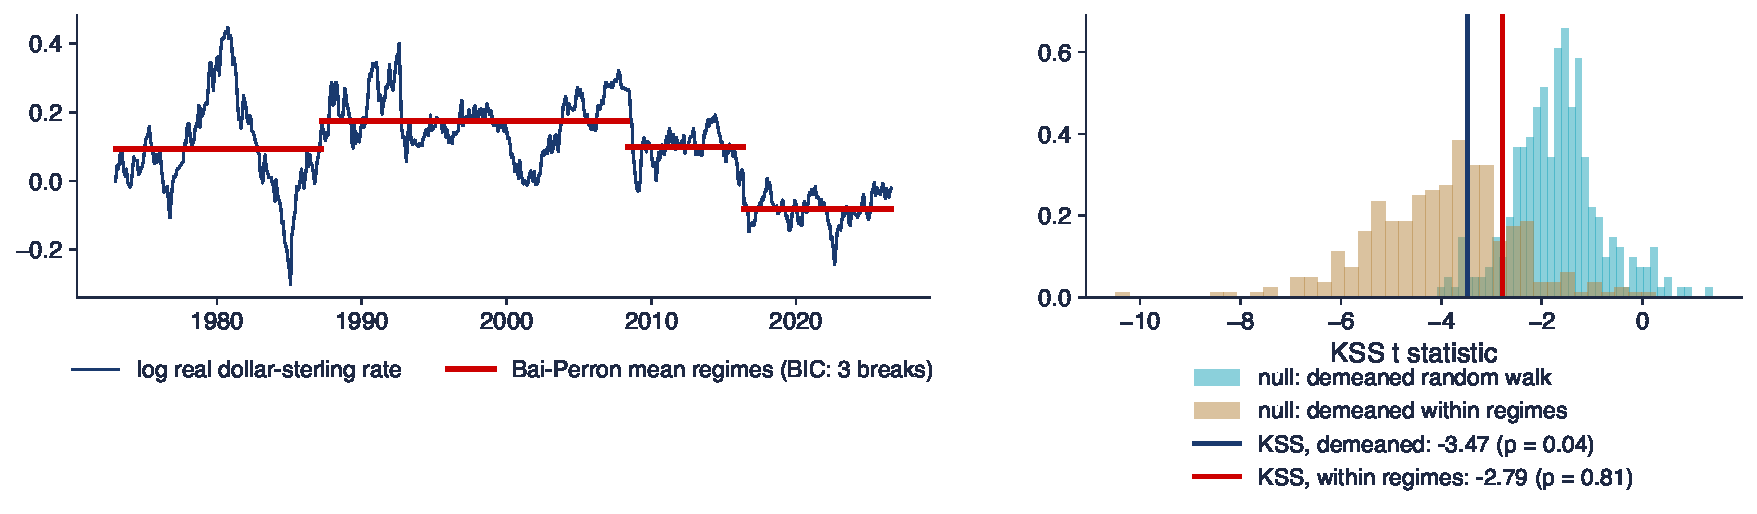
\includegraphics[width=0.97\textwidth,height=0.46\textheight,keepaspectratio]{ats_ch2_ai_case.pdf}
\end{center}
\vspace{-0.25cm}
\begin{itemize}
    \item Stînga: cursul real dolar--liră cu regimurile de medie Bai--Perron (BIC: trei rupturi, martie 1987, mai 2008, mai 2016); dreapta: distribuțiile KSS sub ipoteza nulă din 300 de mersuri aleatoare trecute prin aceiași pași
    \item Cu media scăzută: KSS \ensuremath{-}3{,}47, $p$ 0{,}037 (5\%: \ensuremath{-}3{,}13); în interiorul regimurilor: \ensuremath{-}2{,}79, $p$ 0{,}813 (5\%: \ensuremath{-}6{,}30): dovezile pentru ESTAR dispar odată ce căutarea rupturilor face parte din ipoteza nulă
\end{itemize}
\quantlet{ATS\_ch2\_ai\_case}{\qlurl{ATS_ch2_ai_case}}
\end{frame}

\begin{frame}{Idee de proiect}
\itemsize{\small}
\begin{itemize}
    \item \textbf{Regimuri în inflația din România și în dobînda de politică monetară}: rupturi, praguri sau ambele?
    \begin{itemize}
        \item replicați întîi: datele Bai--Perron din acest curs și testul TAR din \refHb\ pe datele din SUA
        \item extensie: un model AR al inflației din România cu o ruptură parțială în termenul liber, față de un LSTAR în variația pe 12 luni a inflației; preînregistrați comparația (1--12 luni, CRPS, Holm)
        \item opțional: transmiterea cu prag de la dobînda BNR la ROBOR (\atschlink{https://danpele.github.io/Advanced-Time-Series/RO/Cursuri/capitol4_cointegrare_vecm_ardl_panel.pdf}{Capitolul 4})
    \end{itemize}
    \item Livrabilele urmează regulile cursului: repository, raport, AI\_USE.md, AI\_ERRORS.md, susținere orală
\end{itemize}
\end{frame}


%=============================================================================
\section{Încheiere}
%=============================================================================

\begin{frame}{Idei de reținut}
\itemsize{\small}
\begin{itemize}
    \item O dată a rupturii aleasă din date este un parametru neidentificat: folosiți testele sup/exp/ave cu valorile lor critice
    \item Bai--Perron: cele mai mici pătrate globale prin programare dinamică, UDmax și teste secvențiale, BIC/LWZ, intervale pentru date
    \item Monitorizați cu o frontieră CSW; testați rupturile în varianță cu $\kappa_2$; folosiți bootstrap pentru testele de rădăcină unitară cu rupturi
    \item TAR și STAR: testați cu bootstrap sau cu dezvoltări LM, estimați prin (N)LS concentrate, prognozați prin simulare
    \item Rupturile și neliniaritatea se imită reciproc: testați-o pe una ținînd cont de cealaltă
\end{itemize}
\end{frame}

\begin{frame}{Autoevaluare}
\itemsize{\small}
\begin{columns}[T]
\begin{column}{0.56\textwidth}
\begin{block}{Întrebări}
\begin{itemize}
    \item De ce este valoarea critică de 5\% a sup-Wald cu un coeficient peste 8, nu 3,84?
    \item Ce economisește programarea dinamică în estimatorul Bai--Perron?
    \item De ce dă pînă la urmă o alarmă falsă un test de 5\% repetat?
    \item De ce se estimează pragul unui TAR cu rata $T$?
    \item Cînd depinde timpul de înjumătățire al unui ESTAR de șoc?
\end{itemize}
\end{block}
\end{column}
\begin{column}{0.40\textwidth}
\begin{block}{Urmează: VAR structural și proiecții locale}
\begin{itemize}
    \item Modele VAR structurale și proiecții locale: identificarea șocurilor
    \item Proiecțiile locale dependente de stare extind modelele neliniare din acest capitol la răspunsurile la impuls
\end{itemize}
\end{block}
\end{column}
\end{columns}
\end{frame}


%=============================================================================
\section{Anexă}
%=============================================================================

\begin{frame}{Anexă: limita statisticii sup-Wald}
\hypertarget{atsapp1}{}\atsappback{atssrc1}{Înapoi}
\itemsize{\small}
\begin{itemize}
    \item Schimbare de medie, $\sigma^2$ cunoscut: $W_T(\pi) = \dfrac{T\pi(1 - \pi)(\bar y_1 - \bar y_2)^2}{\sigma^2}$, $\bar y_1$, $\bar y_2$ mediile înainte și după $[\pi T]$
    \item Cu $S_T(r) = \sigma^{-1}T^{-1/2}\sum_{t \le [rT]}(y_t - \mu) \Rightarrow B(r)$ (FCLT, \atschlink{https://danpele.github.io/Advanced-Time-Series/RO/Cursuri/capitol0_recapitulare_inferenta.pdf}{Capitolul 0}): $\bar y_1 - \bar y_2 = \dfrac{\sigma}{\sqrt T}\Big[\dfrac{S_T(\pi)}{\pi} - \dfrac{S_T(1) - S_T(\pi)}{1 - \pi}\Big]$
    \item Paranteza este egală cu $\dfrac{S_T(\pi) - \pi S_T(1)}{\pi(1 - \pi)}$, deci $W_T(\pi) \Rightarrow \dfrac{[B(\pi) - \pi B(1)]^2}{\pi(1 - \pi)}$, o punte browniană la pătrat împărțită la varianța ei
    \item Teorema funcțiilor continue dă limita lui $\sup_{\pi \in \Pi}$; cu $p$ coeficienți, $B$ este $p$-dimensională; cu $\sigma^2$ necunoscut sau cu varianță HAC limita este aceeași
\end{itemize}
\end{frame}

\begin{frame}{Anexă: valoarea critică 7,35 a LR pentru prag}
\hypertarget{atsapp2}{}\atsappback{atssrc2}{Înapoi}
\itemsize{\small}
\begin{itemize}
    \item \refHc: cu un efect de prag care scade, $\mathrm{LR}_T(\gamma_0) \to_d \eta^2\xi$, $\xi = \max_{s}[2W(s) - |s|]$, $W$ o mișcare browniană bilaterală
    \item Pentru o parte, $\max_{s \ge 0}[2W(s) - s]$ este exponențial cu media 2: $P(\cdot \le x) = 1 - e^{-x/2}$ (maximul unei mișcări browniene cu derivă)
    \item Cele două părți sînt independente: $P(\xi \le x) = (1 - e^{-x/2})^2$; din $(1 - e^{-x/2})^2 = 1 - \alpha$ rezultă $c(\alpha) = -2\ln(1 - \sqrt{1 - \alpha})$
    \item $c(0{,}10) = 5{,}94$, $c(0{,}05) = 7{,}35$, $c(0{,}01) = 10{,}59$; sub heteroscedasticitate împărțim LR la $\hat\eta^2$ înainte de comparare
\end{itemize}
\end{frame}

\begin{frame}{Anexă: dezvoltarea Taylor din spatele LM3}
\hypertarget{atsapp3}{}\atsappback{atssrc3}{Înapoi}
\itemsize{\small}
\begin{itemize}
    \item LSTAR: $G(s; \gamma, c) - \tfrac12 = \tfrac14\gamma(s - c) - \tfrac{1}{48}\gamma^3(s - c)^3 + O(\gamma^5)$ în jurul lui $\gamma = 0$ (cu $\hat\sigma_s = 1$)
    \item Înlocuind în $\phi_1'\mathbf x_t + (\phi_2 - \phi_1)'\mathbf x_t G$ și grupînd puterile lui $s_t$ obținem $\beta_0'\mathbf x_t + \sum_{k=1}^3\beta_k'\tilde{\mathbf x}_t s_t^k$, fiecare $\beta_k$ proporțional cu $\gamma$
    \item Deci $H_0$: $\gamma = 0$ devine $\beta_1 = \beta_2 = \beta_3 = 0$, testabilă fără a estima $c$; dezvoltarea de ordinul întîi (LM1) nu are putere cînd comută doar termenul liber \refLST
    \item ESTAR: $1 - e^{-\gamma(s - c)^2} = \gamma(s - c)^2 + O(\gamma^2)$: doar pătrate, de aici regula de decizie din \refTer
\end{itemize}
\end{frame}


%=============================================================================
\section{Bibliografie}
%=============================================================================

\begin{frame}{Bibliografie (1/6)}
\itemsize{\tiny}
\begin{itemize}
    \item Andrews, D. W. K. (1993). Tests for parameter instability and structural change with unknown change point. \textit{Econometrica}, 61(4), 821--856. \href{https://doi.org/10.2307/2951764}{doi:10.2307/2951764}
    \item Andrews, D. W. K., \& Ploberger, W. (1994). Optimal tests when a nuisance parameter is present only under the alternative. \textit{Econometrica}, 62(6), 1383--1414. \href{https://doi.org/10.2307/2951753}{doi:10.2307/2951753}
    \item Bai, J. (1997). Estimation of a change point in multiple regression models. \textit{The Review of Economics and Statistics}, 79(4), 551--563. \href{https://doi.org/10.1162/003465397557132}{doi:10.1162/003465397557132}
    \item Bai, J., \& Perron, P. (1998). Estimating and testing linear models with multiple structural changes. \textit{Econometrica}, 66(1), 47--78. \href{https://doi.org/10.2307/2998540}{doi:10.2307/2998540}
    \item Bai, J., \& Perron, P. (2003). Computation and analysis of multiple structural change models. \textit{Journal of Applied Econometrics}, 18(1), 1--22. \href{https://doi.org/10.1002/jae.659}{doi:10.1002/jae.659}
    \item Balke, N. S., \& Fomby, T. B. (1997). Threshold cointegration. \textit{International Economic Review}, 38(3), 627--645. \href{https://doi.org/10.2307/2527284}{doi:10.2307/2527284}
    \item Brock, W. A., Dechert, W. D., Scheinkman, J. A., \& LeBaron, B. (1996). A test for independence based on the correlation dimension. \textit{Econometric Reviews}, 15(3), 197--235. \href{https://doi.org/10.1080/07474939608800353}{doi:10.1080/07474939608800353}
    \item Brown, R. L., Durbin, J., \& Evans, J. M. (1975). Techniques for testing the constancy of regression relationships over time. \textit{Journal of the Royal Statistical Society, Series B}, 37(2), 149--192. \href{https://doi.org/10.1111/j.2517-6161.1975.tb01532.x}{doi:10.1111/j.2517-6161.1975.tb01532.x}
    \item Carrasco, M. (2002). Misspecified structural change, threshold, and Markov-switching models. \textit{Journal of Econometrics}, 109(2), 239--273. \href{https://doi.org/10.1016/S0304-4076(02)00112-4}{doi:10.1016/S0304-4076(02)00112-4}
    \item Casini, A., \& Perron, P. (2019). Structural breaks in time series. In \textit{Oxford Research Encyclopedia of Economics and Finance}. Oxford University Press. \href{https://doi.org/10.1093/acrefore/9780190625979.013.179}{doi:10.1093/acrefore/9780190625979.013.179}
    \item Chan, K. S. (1993). Consistency and limiting distribution of the least squares estimator of a threshold autoregressive model. \textit{The Annals of Statistics}, 21(1), 520--533. \href{https://doi.org/10.1214/aos/1176349040}{doi:10.1214/aos/1176349040}
    \item Chow, G. C. (1960). Tests of equality between sets of coefficients in two linear regressions. \textit{Econometrica}, 28(3), 591--605. \href{https://doi.org/10.2307/1910133}{doi:10.2307/1910133}
\end{itemize}
\end{frame}

\begin{frame}{Bibliografie (2/6)}
\itemsize{\tiny}
\begin{itemize}
    \item Chu, C.-S. J., Hornik, K., \& Kuan, C.-M. (1995). MOSUM tests for parameter constancy. \textit{Biometrika}, 82(3), 603--617. \href{https://doi.org/10.1093/biomet/82.3.603}{doi:10.1093/biomet/82.3.603}
    \item Chu, C.-S. J., Stinchcombe, M., \& White, H. (1996). Monitoring structural change. \textit{Econometrica}, 64(5), 1045--1065. \href{https://doi.org/10.2307/2171955}{doi:10.2307/2171955}
    \item Clements, M. P., Franses, P. H., \& Swanson, N. R. (2004). Forecasting economic and financial time-series with non-linear models. \textit{International Journal of Forecasting}, 20(2), 169--183. \href{https://doi.org/10.1016/j.ijforecast.2003.10.004}{doi:10.1016/j.ijforecast.2003.10.004}
    \item Clements, M. P., \& Hendry, D. F. (1998). \textit{Forecasting Economic Time Series}. Cambridge University Press. \href{https://doi.org/10.1017/CBO9780511599286}{doi:10.1017/CBO9780511599286}
    \item Clements, M. P., \& Hendry, D. F. (2006). Forecasting with breaks. In G. Elliott, C. W. J. Granger, \& A. Timmermann (Eds.), \textit{Handbook of Economic Forecasting} (Vol.\ 1, pp.\ 605--657). Elsevier. \href{https://doi.org/10.1016/S1574-0706(05)01012-8}{doi:10.1016/S1574-0706(05)01012-8}
    \item Davies, R. B. (1987). Hypothesis testing when a nuisance parameter is present only under the alternative. \textit{Biometrika}, 74(1), 33--43. \href{https://doi.org/10.1093/biomet/74.1.33}{doi:10.1093/biomet/74.1.33}
    \item Diebold, F. X., \& Inoue, A. (2001). Long memory and regime switching. \textit{Journal of Econometrics}, 105(1), 131--159. \href{https://doi.org/10.1016/S0304-4076(01)00073-2}{doi:10.1016/S0304-4076(01)00073-2}
    \item Diebold, F. X., \& Mariano, R. S. (1995). Comparing predictive accuracy. \textit{Journal of Business \& Economic Statistics}, 13(3), 253--263. \href{https://doi.org/10.1080/07350015.1995.10524599}{doi:10.1080/07350015.1995.10524599}
    \item van Dijk, D., Teräsvirta, T., \& Franses, P. H. (2002). Smooth transition autoregressive models: A survey of recent developments. \textit{Econometric Reviews}, 21(1), 1--47. \href{https://doi.org/10.1081/ETC-120008723}{doi:10.1081/ETC-120008723}
    \item Eitrheim, Ø., \& Teräsvirta, T. (1996). Testing the adequacy of smooth transition autoregressive models. \textit{Journal of Econometrics}, 74(1), 59--75. \href{https://doi.org/10.1016/0304-4076(95)01751-8}{doi:10.1016/0304-4076(95)01751-8}
    \item Enders, W., \& Siklos, P. L. (2001). Cointegration and threshold adjustment. \textit{Journal of Business \& Economic Statistics}, 19(2), 166--176. \href{https://doi.org/10.1198/073500101316970395}{doi:10.1198/073500101316970395}
    \item Fryzlewicz, P. (2014). Wild binary segmentation for multiple change-point detection. \textit{The Annals of Statistics}, 42(6), 2243--2281. \href{https://doi.org/10.1214/14-AOS1245}{doi:10.1214/14-AOS1245}
\end{itemize}
\end{frame}

\begin{frame}{Bibliografie (3/6)}
\itemsize{\tiny}
\begin{itemize}
    \item Garcia, R., \& Perron, P. (1996). An analysis of the real interest rate under regime shifts. \textit{The Review of Economics and Statistics}, 78(1), 111--125. \href{https://doi.org/10.2307/2109851}{doi:10.2307/2109851}
    \item Giacomini, R., \& Rossi, B. (2009). Detecting and predicting forecast breakdowns. \textit{The Review of Economic Studies}, 76(2), 669--705. \href{https://doi.org/10.1111/j.1467-937X.2009.00545.x}{doi:10.1111/j.1467-937X.2009.00545.x}
    \item Giacomini, R., \& Rossi, B. (2010). Forecast comparisons in unstable environments. \textit{Journal of Applied Econometrics}, 25(4), 595--620. \href{https://doi.org/10.1002/jae.1177}{doi:10.1002/jae.1177}
    \item Hamilton, J. D. (1994). \textit{Time Series Analysis}. Princeton University Press. \href{https://doi.org/10.2307/j.ctv14jx6sm}{doi:10.2307/j.ctv14jx6sm}
    \item Hansen, B. E. (1996). Inference when a nuisance parameter is not identified under the null hypothesis. \textit{Econometrica}, 64(2), 413--430. \href{https://doi.org/10.2307/2171789}{doi:10.2307/2171789}
    \item Hansen, B. E. (1997). Inference in TAR models. \textit{Studies in Nonlinear Dynamics \& Econometrics}, 2(1). \href{https://doi.org/10.2202/1558-3708.1024}{doi:10.2202/1558-3708.1024}
    \item Hansen, B. E. (2000). Sample splitting and threshold estimation. \textit{Econometrica}, 68(3), 575--603. \href{https://doi.org/10.1111/1468-0262.00124}{doi:10.1111/1468-0262.00124}
    \item Hansen, B. E. (2001). The new econometrics of structural change: Dating breaks in U.S. labor productivity. \textit{Journal of Economic Perspectives}, 15(4), 117--128. \href{https://doi.org/10.1257/jep.15.4.117}{doi:10.1257/jep.15.4.117}
    \item Hansen, B. E. (2011). Threshold autoregression in economics. \textit{Statistics and Its Interface}, 4(2), 123--127. \href{https://doi.org/10.4310/SII.2011.v4.n2.a4}{doi:10.4310/SII.2011.v4.n2.a4}
    \item Hansen, B. E., \& Seo, B. (2002). Testing for two-regime threshold cointegration in vector error-correction models. \textit{Journal of Econometrics}, 110(2), 293--318. \href{https://doi.org/10.1016/S0304-4076(02)00097-0}{doi:10.1016/S0304-4076(02)00097-0}
    \item Harvey, D., Leybourne, S., \& Newbold, P. (1997). Testing the equality of prediction mean squared errors. \textit{International Journal of Forecasting}, 13(2), 281--291. \href{https://doi.org/10.1016/S0169-2070(96)00719-4}{doi:10.1016/S0169-2070(96)00719-4}
    \item Huang, C., \& Petukhina, A. (2022). \textit{Applied Time Series Analysis and Forecasting with Python}. Springer. \href{https://doi.org/10.1007/978-3-031-13584-2}{doi:10.1007/978-3-031-13584-2}
\end{itemize}
\end{frame}

\begin{frame}{Bibliografie (4/6)}
\itemsize{\tiny}
\begin{itemize}
    \item Inclán, C., \& Tiao, G. C. (1994). Use of cumulative sums of squares for retrospective detection of changes of variance. \textit{Journal of the American Statistical Association}, 89(427), 913--923. \href{https://doi.org/10.1080/01621459.1994.10476824}{doi:10.1080/01621459.1994.10476824}
    \item Inoue, A., Jin, L., \& Rossi, B. (2017). Rolling window selection for out-of-sample forecasting with time-varying parameters. \textit{Journal of Econometrics}, 196(1), 55--67. \href{https://doi.org/10.1016/j.jeconom.2016.03.006}{doi:10.1016/j.jeconom.2016.03.006}
    \item Kapetanios, G., Shin, Y., \& Snell, A. (2003). Testing for a unit root in the nonlinear STAR framework. \textit{Journal of Econometrics}, 112(2), 359--379. \href{https://doi.org/10.1016/S0304-4076(02)00202-6}{doi:10.1016/S0304-4076(02)00202-6}
    \item Kilian, L., \& Lütkepohl, H. (2017). \textit{Structural Vector Autoregressive Analysis}. Cambridge University Press. \href{https://doi.org/10.1017/9781108164818}{doi:10.1017/9781108164818}
    \item Killick, R., Fearnhead, P., \& Eckley, I. A. (2012). Optimal detection of changepoints with a linear computational cost. \textit{Journal of the American Statistical Association}, 107(500), 1590--1598. \href{https://doi.org/10.1080/01621459.2012.737745}{doi:10.1080/01621459.2012.737745}
    \item Kim, D., \& Perron, P. (2009). Unit root tests allowing for a break in the trend function at an unknown time under both the null and alternative hypotheses. \textit{Journal of Econometrics}, 148(1), 1--13. \href{https://doi.org/10.1016/j.jeconom.2008.08.019}{doi:10.1016/j.jeconom.2008.08.019}
    \item Koop, G., \& Potter, S. M. (1999). Dynamic asymmetries in U.S. unemployment. \textit{Journal of Business \& Economic Statistics}, 17(3), 298--312. \href{https://doi.org/10.1080/07350015.1999.10524819}{doi:10.1080/07350015.1999.10524819}
    \item Lee, J., \& Strazicich, M. C. (2003). Minimum Lagrange multiplier unit root test with two structural breaks. \textit{The Review of Economics and Statistics}, 85(4), 1082--1089. \href{https://doi.org/10.1162/003465303772815961}{doi:10.1162/003465303772815961}
    \item Liu, J., Wu, S., \& Zidek, J. V. (1997). On segmented multivariate regression. \textit{Statistica Sinica}, 7(2), 497--525. \href{https://www3.stat.sinica.edu.tw/statistica/j7n2/j7n213/j7n213.htm}{www3.stat.sinica.edu.tw}
    \item Lumsdaine, R. L., \& Papell, D. H. (1997). Multiple trend breaks and the unit-root hypothesis. \textit{The Review of Economics and Statistics}, 79(2), 212--218. \href{https://doi.org/10.1162/003465397556791}{doi:10.1162/003465397556791}
    \item Luukkonen, R., Saikkonen, P., \& Teräsvirta, T. (1988). Testing linearity against smooth transition autoregressive models. \textit{Biometrika}, 75(3), 491--499. \href{https://doi.org/10.1093/biomet/75.3.491}{doi:10.1093/biomet/75.3.491}
    \item McConnell, M. M., \& Perez-Quiros, G. (2000). Output fluctuations in the United States: What has changed since the early 1980's? \textit{American Economic Review}, 90(5), 1464--1476. \href{https://doi.org/10.1257/aer.90.5.1464}{doi:10.1257/aer.90.5.1464}
\end{itemize}
\end{frame}

\begin{frame}{Bibliografie (5/6)}
\itemsize{\tiny}
\begin{itemize}
    \item Michael, P., Nobay, A. R., \& Peel, D. A. (1997). Transactions costs and nonlinear adjustment in real exchange rates: An empirical investigation. \textit{Journal of Political Economy}, 105(4), 862--879. \href{https://doi.org/10.1086/262096}{doi:10.1086/262096}
    \item Montgomery, A. L., Zarnowitz, V., Tsay, R. S., \& Tiao, G. C. (1998). Forecasting the U.S. unemployment rate. \textit{Journal of the American Statistical Association}, 93(442), 478--493. \href{https://doi.org/10.1080/01621459.1998.10473696}{doi:10.1080/01621459.1998.10473696}
    \item Neftçi, S. N. (1984). Are economic time series asymmetric over the business cycle? \textit{Journal of Political Economy}, 92(2), 307--328. \href{https://doi.org/10.1086/261226}{doi:10.1086/261226}
    \item Oka, T., \& Perron, P. (2018). Testing for common breaks in a multiple equations system. \textit{Journal of Econometrics}, 204(1), 66--85. \href{https://doi.org/10.1016/j.jeconom.2018.01.003}{doi:10.1016/j.jeconom.2018.01.003}
    \item Perron, P. (1989). The great crash, the oil price shock, and the unit root hypothesis. \textit{Econometrica}, 57(6), 1361--1401. \href{https://doi.org/10.2307/1913712}{doi:10.2307/1913712}
    \item Pesaran, M. H., \& Pick, A. (2011). Forecast combination across estimation windows. \textit{Journal of Business \& Economic Statistics}, 29(2), 307--318. \href{https://doi.org/10.1198/jbes.2010.09018}{doi:10.1198/jbes.2010.09018}
    \item Pesaran, M. H., \& Timmermann, A. (2007). Selection of estimation window in the presence of breaks. \textit{Journal of Econometrics}, 137(1), 134--161. \href{https://doi.org/10.1016/j.jeconom.2006.03.010}{doi:10.1016/j.jeconom.2006.03.010}
    \item Petropoulos, F., Apiletti, D., Assimakopoulos, V., et al.\ (2022). Forecasting: theory and practice. \textit{International Journal of Forecasting}, 38(3), 705--871. \href{https://doi.org/10.1016/j.ijforecast.2021.11.001}{doi:10.1016/j.ijforecast.2021.11.001}
    \item Ploberger, W., \& Krämer, W. (1992). The CUSUM test with OLS residuals. \textit{Econometrica}, 60(2), 271--285. \href{https://doi.org/10.2307/2951597}{doi:10.2307/2951597}
    \item Quandt, R. E. (1960). Tests of the hypothesis that a linear regression system obeys two separate regimes. \textit{Journal of the American Statistical Association}, 55(290), 324--330. \href{https://doi.org/10.1080/01621459.1960.10482067}{doi:10.1080/01621459.1960.10482067}
    \item Robbins, H., \& Siegmund, D. (1970). Boundary crossing probabilities for the Wiener process and sample sums. \textit{The Annals of Mathematical Statistics}, 41(5), 1410--1429. \href{https://doi.org/10.1214/aoms/1177696787}{doi:10.1214/aoms/1177696787}
    \item Rossi, B. (2013). Advances in forecasting under instability. In G. Elliott \& A. Timmermann (Eds.), \textit{Handbook of Economic Forecasting} (Vol.\ 2B, pp.\ 1203--1324). Elsevier. \href{https://doi.org/10.1016/B978-0-444-62731-5.00021-X}{doi:10.1016/B978-0-444-62731-5.00021-X}
\end{itemize}
\end{frame}

\begin{frame}{Bibliografie (6/6)}
\itemsize{\tiny}
\begin{itemize}
    \item Sansó, A., Aragó, V., \& Carrion, J. L. (2004). Testing for changes in the unconditional variance of financial time series. \textit{Revista de Economía Financiera}, 4, 32--52. \href{https://econpapers.repec.org/RePEc:ubi:deawps:5}{econpapers.repec.org}
    \item Stock, J. H., \& Watson, M. W. (1996). Evidence on structural instability in macroeconomic time series relations. \textit{Journal of Business \& Economic Statistics}, 14(1), 11--30. \href{https://doi.org/10.1080/07350015.1996.10524626}{doi:10.1080/07350015.1996.10524626}
    \item Taylor, M. P., Peel, D. A., \& Sarno, L. (2001). Nonlinear mean-reversion in real exchange rates: Toward a solution to the purchasing power parity puzzles. \textit{International Economic Review}, 42(4), 1015--1042. \href{https://doi.org/10.1111/1468-2354.00144}{doi:10.1111/1468-2354.00144}
    \item Teräsvirta, T. (1994). Specification, estimation, and evaluation of smooth transition autoregressive models. \textit{Journal of the American Statistical Association}, 89(425), 208--218. \href{https://doi.org/10.1080/01621459.1994.10476462}{doi:10.1080/01621459.1994.10476462}
    \item Teräsvirta, T., van Dijk, D., \& Medeiros, M. C. (2005). Linear models, smooth transition autoregressions, and neural networks for forecasting macroeconomic time series: A re-examination. \textit{International Journal of Forecasting}, 21(4), 755--774. \href{https://doi.org/10.1016/j.ijforecast.2005.04.010}{doi:10.1016/j.ijforecast.2005.04.010}
    \item Tong, H., \& Lim, K. S. (1980). Threshold autoregression, limit cycles and cyclical data. \textit{Journal of the Royal Statistical Society, Series B}, 42(3), 245--268. \href{https://doi.org/10.1111/j.2517-6161.1980.tb01126.x}{doi:10.1111/j.2517-6161.1980.tb01126.x}
    \item Truong, C., Oudre, L., \& Vayatis, N. (2020). Selective review of offline change point detection methods. \textit{Signal Processing}, 167, 107299. \href{https://doi.org/10.1016/j.sigpro.2019.107299}{doi:10.1016/j.sigpro.2019.107299}
    \item Tsay, R. S. (1986). Nonlinearity tests for time series. \textit{Biometrika}, 73(2), 461--466. \href{https://doi.org/10.1093/biomet/73.2.461}{doi:10.1093/biomet/73.2.461}
    \item Tsay, R. S. (1989). Testing and modeling threshold autoregressive processes. \textit{Journal of the American Statistical Association}, 84(405), 231--240. \href{https://doi.org/10.1080/01621459.1989.10478760}{doi:10.1080/01621459.1989.10478760}
    \item Zeileis, A., Leisch, F., Hornik, K., \& Kleiber, C. (2002). strucchange: An R package for testing for structural change in linear regression models. \textit{Journal of Statistical Software}, 7(2), 1--38. \href{https://doi.org/10.18637/jss.v007.i02}{doi:10.18637/jss.v007.i02}
    \item Zivot, E., \& Andrews, D. W. K. (1992). Further evidence on the great crash, the oil-price shock, and the unit-root hypothesis. \textit{Journal of Business \& Economic Statistics}, 10(3), 251--270. \href{https://doi.org/10.1080/07350015.1992.10509904}{doi:10.1080/07350015.1992.10509904}
\end{itemize}
\end{frame}

\end{document}
